\documentclass[10pt,a4paper]{book}
\usepackage[utf8]{inputenc}
\usepackage{amsmath}
\usepackage{amsfonts}
\usepackage{amssymb}
\usepackage{placeins}
\usepackage{polski}
\usepackage{natbib}
\usepackage{graphicx}
\usepackage{makeidx}
\usepackage{ifthen}
\usepackage[polish, section]{dyschemist}
%\makeindex
\usepackage[hidelinks]{hyperref}
\usepackage[left=2cm,right=2cm,top=2cm,bottom=2cm]{geometry}


\newcommand{\tsAutoCovariance}[3][\gamma]{\operatorname{#1}_{#2} \left({#3}\right)}
\newcommand{\tsAutoCorellation}[3][\rho]{\operatorname{#1}_{#2} \left({#3}\right)}
\newcommand{\argmax}{\operatornamewithlimits{argmax}}

\usepackage{dyschemist}
\author{dr, mgr inż. Piotr Kowalski}
\title{Skrypt do wykładu z Szeregów czasowych i prognozowanie w biznesie}
\date{\today}
\begin{document}

\begin{titlepage}
\maketitle
\end{titlepage}
\FloatBarrier

\begin{table}[h]
\centering
\begin{tabular}{|p{1cm}|p{2cm}|p{12mm}|p{12cm}|}\hline
Wersja & Autor & Data & Opis\\\hline
0.1 & P.Kowalski & 18.03.18& Utworzenie początkowej wersji skryptu, przygotowanie wstępu oraz wprowadzeniu pojęcia szeregu czasowego,\\\hline
0.2 & P.Kowalski & 26.03.18& Dołączenie pojęć z zakresu stacjonarnego szeregu czasowego oraz metod dekompozycji szeregu do postaci stacjonarnego.\\\hline
0.3 & P. Kowalski & 22.04.18 & Dołączenie informacji o regresji oraz prognozowania szeregów stacjonarnych oraz wstęp do modeli ARIMA \\\hline
0.4 & P. Kowalski & 06.05.18 & Uzupełnienie o modelach ARIMA \\\hline
0.5 & P. Kowalski & 13.05.18 & Dołączenie modelu GARCH \\\hline
0.6 & P. Kowalski & 18.05.18 & Prognozowanie modelami wykładniczymi \\\hline
0.7 & P. Kowalski & 27.05.18 & Przyczynowość Grangera \\\hline
0.8 & P. Kowalski & 3.06.18 & Model VAR \\\hline
0.9 & P. Kowalski & 10.06.18 & Modelowanie niestacjonarnych szeregów \\\hline
1.0 & P. Kowalski & 15.06.18 & Naniesienie poprawek - zamknięcie wersji 1.0, dołączenie indeksów. \\\hline
1.1 & P. Kowalski & 17.06.18 & Poprawki Broniarczyk i Przepióra. \\\hline
1.2 & P. Kowalski & 17.06.18 & Poprawki Stelmachowicz. \\\hline
1.3 & P. Kowalski & 21.06.18 & Poprawki Choja, Heppner, Broniarczyk  \\\hline
1.4 & P. Kowalski & 21.06.18 & Poprawki Mostowska  \\\hline
1.5 & P. Kowalski & 21.06.18 & Poprawki Przepióra, Margielewski  \\\hline
1.6 & P. Kowalski & 03.04.19 & Pierwsze poprawki w kolejnym roku edycji \\\hline
1.7 & P. Kowalski & 10.04.19 & Dodanie elementów do modeli GARCH \\\hline
1.8 & P. Kowalski & 24.04.19 & Dodanie wprowadzenia do procesów decyzyjnych Markowa, oraz predykcji opartej o sieci neuronowe \\\hline
1.9 & P. Kowalski & 28.04.19 & Dodanie elementów dotyczących zastosowania teorii spektralnej do predykcji \\\hline
1.10 & P. Kowalski & 8.05.19 & Rozszerzenie elementów związanych z modelami decyzyjnymi Markowa oraz Q-learningiem \\\hline
\end{tabular}
\caption{Wersje dokumentu.}
\end{table}
\FloatBarrier

\chapter*{Przedmowa}
\addcontentsline{toc}{chapter}{Przedmowa}

Niniejszy skrypt gromadzi materiały przygotowane dla potrzeb kursu z Szeregów czasowych i prognozowania w biznesie dla studentów kierunku matematyka na Politechnice Łódzkiej w roku akademickim 2017/18. W pewnej części został oparty o przygotowany przez dr Elżbietę Krajewska oraz prof. Tadeusza Poredę wykład z lat poprzedzających. Skrypt został w późniejszym czasie mocno przebudowany, tak aby uwzględnić teorie wielowymiarowych modeli szeregów czasowych autorstwa 4 laureatów nagrody im. Nobla z zakresu ekonomii oraz elementy uczenia maszynowe w realizacji zadań predykcji. W roku akademickim 2018/19 planowane jest rozbudowanie skryptu o elementy składni R. 

\newpage
\tableofcontents

\chapter{Wprowadzenie}

\section{Geneza prognozowania}

Każdy z nas słyszał chyba historię o jednym z największych umysłów starożytnego świata - Archimedesie - i jego kąpieli. Część jednak nie pamięta związanej z tym wydarzeniem historii, a jeszcze mniejsza ilość zdaje sobie sprawę z wielkości tamtego odkrycia. Legenda dotycząca tego wydarzenia podaje, iż Archimedes został postawiony przez króla Syrakuz Hierona II przed zadaniem sprawdzenia królewskiego złotnika. Złotnik miał przygotować dla swojego króla koronę ze szczerego złota. Jednak kiedy była już gotowa, nie niszcząc jej nie można było stwierdzić czy złotnik zrealizował zadanie zgodnie z życzeniem, czy też użył domieszek innych metali. Archimedes długo rozważał jak zbadać to zagadnienie, kiedy to ostatecznie zażywając kąpieli odkrył zasadę wypierania wody przez ciało. W przypływie euforii krzycząc 'Eureka' przebiegł nagi ulicami Syrakuz. Z wykorzystaniem zasady wypierania cieczy przez ciało porównano wagi korony oraz równej objętościowo bryły złota i uznano, iż korona zawiera domieszki innych metali. Los oszusta złotnika nie jest historycznie pewny, lecz z pewnością był marny. Eureka - od czasu tego wydarzenia przypisywana była zachwytowi wobec znacznego odkrycia. 

Część historyków\citep{netz2007kodeks} zauważa jednak, że odkrycie z tamtej kąpieli posiada jeszcze głębsze dno jeszcze bardziej doniosłego. Prawo wypierania cieczy stanowi jedno z pierwszych praw fizyki, sformułowanych przez człowieka. Powstało ono po prawdzie niewiele później od pierwszych matematycznych zasad. W chwili gdy Archimedes wyskoczył z okrzykiem z wanny stała się również inna bardziej znamienita rzecz. Odkryta została inżynieria. Połączenie bowiem prawa fizyki z elementami matematyki - po raz pierwszy w historii - pozwoliła człowiekowi patrzeć w przyszłość. Posiadając prawo fizyki oraz rachunek liczb - można było podać wynik pewnego doświadczenia, jeszcze zanim zostało ono przeprowadzone. Znając materiał (jego gęstość i objętość) i wykorzystując prawo wypierania można było podać dokładną ilość wypartej wody. Ta sama zasada pozwoliła sformułować wniosek o tym czy statek z danym obciążeniem będzie mógł unosić się na wodzie. Wtedy właśnie narodziło się jedno z najpotrzebniejszych zastosowań matematyki - tworzenie predykcji lub prognoz - opisu przyszłych wydarzeń na podstawie wiedzy i parametrów z przeszłości i doświadczeń.  

Prognozowanie\index{Prognoza} jest pojęciem pochodzącym już z czasów antycznych, przez niektórych przypisywane Hipokratesowi z Kos (twórcy antycznej medycyny). Gnosis - wiedza po grecku, Prognosis - "przed wiedza", uprzednia wiedza - opisująca wiedzę o zdarzeniach z przyszłości. Z kolei predykcja\index{Predykcja} jest terminem o etymologii typowo rzymskiej (pre-dicere) powiedziane przed - wypowiedziane z wyprzedzeniem.

Współczesne prognozowanie nie przypomina już w zasadzie prognozowania znanego z czasów antycznych. Zjawiska, które obecnie podlegają prognozowaniu z rzadka posiadają charakter deterministycznych praw fizyki. Najczęściej prognozowane obecnie zjawiska posiadają typowy charakter probabilistyczny/stochastyczny. Dokładne wartości zostały zastąpione przez rozkłady prawdopodobieństwa czy opisy histogramowe częstości poszczególnych wartości. Nadal jednak nadrzędną jest zasada, aby wyprzedzić swój czas i podać możliwie najdokładniejszy, najmniej omylny sposób wypowiadania zdań prawdziwych o zjawiskach, które zostaną zaobserwowane w przyszłości.

\section{Podziały prognoz}

Do dwóch głównych nurtów prognozowania zalicza się \citep[Ch. 1]{montgomery2015introduction} prognozowanie jakościowe i ilościowe. Prognozowanie jakościowe\index{Prognoza!jakościowa}, choć może wykorzystywać matematyczne modele i obliczenia, w znacznej mierze opiera się na subiektywnych ocenach formułowanych przez ekspertów. Przykładami zdań wypowiadanych w ramach prognozowania jakościowe są np.
\begin{itemize}
\item Lato będzie upalne,
\item Wartośc firmy będzie dalej wzrastać,
\item Student przedłoży pracę dyplomową w terminie.
\end{itemize}
Z kolei prognozowanie ilościowe\index{Prognoza!ilościowa} wykorzystuje dane historyczne dotyczące zjawiska, tworzy matematyczne modele celem odkrycia zależności pomiędzy bieżącymi, a następującymi wartościami zjawiska. W sposób oczywisty, w niniejszym skrypcie omawiane zostaną jedynie metody z zakresu prognozowania ilościowego. Tu przykładami zdań w tym typie prognozy są:
\begin{itemize}
\item Temperatura jutro wyniesie $19^o$ C.
\item Cena zamknięcia wartości akcji firmy wyniesie 20,52 dolarów $\pm$ 1
dolar z 90 $\%$ prawdopodobieństwem.
\item Panie Profesorze, na przyszły tydzień będzie 25 stron pracy gotowe.
\end{itemize}
W przedmiocie związanym z tym skryptem rozważamy jedynie modele prognozowania ilościowego.

Wśród podziałów prognoz ważne jest również wyszczególnienie podziału na prognozy:
\begin{description}
\item[Krótkoterminowe] - kilkudniowe - spodziewanym wynikiem dokładne opisy ilościowe,\index{Prognoza!krótkoterminowa}
\item[Średnioterminowe] - od kilkudziesięciu dni do 3 miesięcy - spodziewanym wynikiem są mieszane wyniki ilościowe i jakościowe, \index{Prognoza!średnioterminowa}
\item[Długoterminowe] - o dowolnym dłuższym okresie - ze spodziewanym wynikiem wypowiedzianym jakościowo. \index{Prognoza!długoterminowa}
\end{description}
Naturalnie często granice tego podziału przesuwają się w zależności od omawianego zjawiska - w sposób indywidualnie reprezentujący zmienność danego zjawiska. Im wyższa ta wewnętrzna niepewność tym naturalnie terminy przesuwają swoje granice do wcześniejszych chwil czasu, np. prognoza pogody krótkoterminowa dotyczy prognozy na maksymalnie 2 dni wprzód, a prognoza ponad 16 dni jest już prognozą długoterminową.

\section{Proces tworzenia prognozy}

Nadzorując zespoły analityków pracujące nad opracowaniem kolejnych prognoz obserwujemy wytworzony na drodze współpracy i dobrych praktyk - model procesu tworzenia prognozy\index{Prognoza!proces tworzenia}. W modelu tym kolejne kroki opisują \citep[Sec. 1.3]{montgomery2015introduction}

\begin{enumerate}
\item Opisanie problemu,
\item Zgromadzenie danych,
\item Analiza zbioru danych,
\item Wybór oraz dostrajanie modelu,
\item Weryfikacja poprawności modelu,
\item Wdrożenie modelu,
\item Utrzymywanie i monitorowanie wydajności modelu.
\end{enumerate}

Opisanie problemu dotyczy w głównej mierze zrozumienia oczekiwań po stronie klienta, wskazania konkretnych informacji potrzebnych w prognozie, zakresów prognozy, jej dokładności. Jest to również faza, w której rozsądnym jest wykorzystanie ekspertów z dziedziny, celem wyszczególnienia kluczowych aspektów. Często ważnym, a nieoczywistym elementem tego etapu, jest uświadomienie klientom ryzyka związanego w wykorzystaniem prognozy.

Gromadzenie danych jest procesem mającym na celu zebranie informacji w formacie preferowanym do przetwarzania, dotyczącym historycznych wartości danego zjawiska oraz historycznych wartości potencjalnych czynników je warunkujących. Ważnym jest aby grupować tylko dane istotne - oraz dokładnie monitorować gromadzone dane pod kątem obarczenia ich błędami różnych typów, jak np.
\begin{itemize}
\item Błędu przetwarzania - pojawiającego się wskutek błędu przy kopiowaniu lub transformowaniu danych,\index{Błąd!przetwarzania}
\item Błędów odczytu - reprezentowanych przez wartości odstające w zbiorze danych, \index{Błąd!odczytu}
\item Błędu brakujących wartości. \index{Błąd!brakujących wartości}
\end{itemize}
Na tym etapie często też projektowane są odpowiednie struktury do gromadzenia i przetwarzania tych danych w przyszłości po wdrożeniu modelu.

Analiza zbioru danych - dotyczy stosowania wszelakich metod analizy począwszy od konsultacji z ekspertami, gromadzeniu informacji o zjawiskach opisywanych przez dane, aż po efekty eksperymentów i algorytmów analizy danych. Podstawowym narzędziem do analizy są wszelakie sposoby wizualizacji danych, głównie wykresów. Na tym etapie poszukiwane są również trendy czasowe tak stałe, cykliczne co i sezonowe. Wyznaczane są również całe zbiory charakterystyk opisujących zbiór danych jak: średnie, mediany, mody, kwartyle etc. Efektem porządanym w tym etapie jest zrozumienie specyfiki zjawiska oraz związków nimi rządzących.

Wybór i dostrajanie modelu \index{Model!dostrajanie} - jest iteracyjnym etapem w procesie prognozowania. W kolejnych iteracjach proponowane są różne modele matematyczne - uzyskiwane na podstawie wyników z poprzedzającej ten etap analizy. Modele te mogę różnić się w wielu aspektach. Mogą przyświecać im zupełnie różne koncepcje, różnić się użytymi algorytmami, przekazywanymi czynnikami, aż po różnice w ilości parametrów modelu. Po wyborze modelu przeprowadzane jest dostrajanie modelu, zwane też często uczeniem. W procesie tym wyznaczane są optymalne wartości parametrów - zapewniające minimalizację pewnego rodzaju błędu (zazwyczaj średniokwadratowego). Po wybraniu i dostrojeniu modelu podlega on szybkiej ocenie - i w przypadku niespełnienia podstawowych wymogów postawionych na etapie definiowania - odrzuceniu modelu.

Weryfikacja modelu - istotnie różni się od oceny modelu po jego strojeniu. Tu wiadomym jest już, że określony model spełnia podstawowe wymogi z etapu definicji. Etap ten ma sformułować wnioski dotyczące użycia tego modelu, jego zachowaniu w środowisku produkcyjnym, co on oznacza z punktu modelowania określonego zjawiska. Oceniane są również podatności modelu na wprowadzanie różnych rodzajów danych oraz analiza jakościowa oferowanego przez niego wyjścia. Etap ten w krótkich słowach określa zrozumienie co dla zjawiska oznacza dany model oraz zgromadzenie informacji o silnych i słabych stronach tego modelu. Czasami na tym etapie dochodzi również do porównania kilku akceptowalnych modeli z poprzedzającego etapu.

Etap wdrożenia to procesy głównie związane z Knowledge-Transfer (KT) \index{KT} - przekazania zdobytej wiedzy do klienta, wsparcia lub przeprowadzenia procesu wdrożenia modelu proponowanego w prognozie. Dotyczy to również przeprowadzenia odpowiedniego instruktażu dla klienta - aby mógł z sukcesami korzystać z modelu.

Ostatni etap utrzymywania i monitorowania wydajności modelu - dotyczy uzyskiwania informacji o wydajności modelu w realizacji zadań produkcyjnych. W umysłach twórców prognozy musi występować bowiem świadomość, że modele  -również i te gotowe, wdrożone, produkcyjne - z czasem potrafią na skutek zmian w otaczającym świecie, podlegać dezaktualizacji. Podstawowe wskazanie o tym iż model przestaje zachowywać sie w sposób należyty może być zaobserwowany np. z wykorzystaniem odpowiednich wykresów monitorujących.

\section{Modele naiwne prognozowania i oznaczenia}

Wprowadźmy podstawowe oznaczenia niezbędne do zapisywania prognoz.

\begin{definition}[Oznaczenie prognozy \citep{montgomery2015introduction}]\index{Prognoza!symbol}
Niech $\sequence{y_t}{t}{} $ będzie ciągiem wartości pewnego zjawiska w danej t-tej kolejnej chwili czasu. Prognozę na chwilę czasu $t \in T$ z wyprzedzeniem o $\gamma \in \setN$ oznaczać będziemy symbolem $\predict[t-\gamma]{y}{t}$. W szczególnym przypadku gdy $\gamma =1$ pisać będziemy $\predict{y}{t}= \predict[t-1]{y}{t}$.
\end{definition}

Wprowadźmy również od razu oznaczenie dla błędu danej prognozy

\begin{definition}[Błąd prognozy \citep{montgomery2015introduction}]\index{Błąd!prognozy}
Niech $\sequence{y_t}{t}{} $ będzie ciągiem opisującym pewne zjawisko w kolejnych chwilach czasu a $\predict[t-\gamma]{y}{t}$ jego prognozą o wyprzedzeniu $\gamma \in \setN$. Błędem $\gamma$-prognozy nazywać będziemy ciąg wartości dla kolejnych chwil czasu opisany wzorem:
$$
\sequence{\function[{e_t}]{\gamma}}{t}{} = \sequence{y_t}{t}{} - \sequence{\predict[t-\gamma]{y}{t}}{t}{}.
$$
Analogicznie jak w przypadku prognozy przez $\sequence{e_t}{t}{} = \sequence{\function[{e_t}]{1} }{t}{} $. Ponadto ciąg $\sequence{e_t}{t}{} $ nazywa sie ciągiem rezyduów\index{Szereg!rezydualny}, albo rezydualnym.
\end{definition}

Najprostszym sposobem tworzenia predykcji wg modelu probabilistyczne jest użycie modelu prognozy naiwnej.

\begin{definition}[Prognoza naiwna]\index{Prognoza!naiwna}
Najprostszym modelem prognozowania jest prognoza naiwna w której
$$
\predict{y}{t} = y_{t-1}.
$$
\end{definition}


W prognozie naiwnej za spodziewaną wartość przyjmujemy dokładnie wartość bezpośrednio ją poprzedzającą. Nazywana jest ona naiwną gdyż:
\begin{itemize}
\item Niezależnie od danych zawsze proponuje to samo rozwiązanie,
\item Parametry modelu nie zależą od danych,
\item Dopuszczone są jedynie zależności od bezpośrednio poprzedzającej wartości i to w postaci stałej.
\end{itemize}

%TODO do sprawdzenia w kolejnej edycji - to jest góra jakieś głębszej teorii (https://www.youtube.com/watch?v=fhjJWI7rw2A)
\begin{definition}[Statystyka Theil'a]
Dowolną prognozę można porównać jakościowo z prognozą naiwną wyznaczając wartość następującej statystyki - nazywanej statystyką Theil'a:
$$
U^2 = \frac{\sum_{t = 1}^{T} \bracket{\predict{y}{t+1} - y_t }^2}{\sum_{t=1}^{T} y_t^2}.
$$
\end{definition}
Wartości statystyki Theil'a wyraźnie poniżej $1$ sygnalizują, że metoda predykcji jest skuteczniejsza od prognozy naiwnej.

\section{Metody oceny jakości modelu predykcyjnego}

Niniejsza sekcja została przygotowana z wykorzystaniem \citep{montgomery2015introduction}.

Ostatecznie, w różnej konfiguracji, zaproponowany i wdrożony zostanie model dokonujący dekompozycji i kompozycji wg założonego schematu. Jedynym co pozostanie będzie ocena skuteczności modelu. Nie wskazywanym jest stosowanie tylko jednego sposobu agregowania błędu z modelu. Najczęściej posługujemy się całymi zestawami wskaźników błędu i próbujemy dokonać ich jednoczesnej minimalizacji. W niniejszej sekcji przedstawmy kilka podstawowych sposobów na wprowadzenie błędu prognozy.

\begin{definition}[Różne rodzaje błędu]
Niech $\sequence{y_t}{t}{} $ będzie szeregiem czasowym  o długości $n$ oraz $\predict{y}{t}$ będzie predykcja na 1-okres wprzód. Zgodnie z wprowadzonymi oznaczeniemi $e_t = y_t - \predict{y}{t}$. Wtedy
\begin{itemize}
\item Średnim błędem (ME) nazwiemy \index{Błąd!ME}
$$
ME = \frac{1}{n} \sum  e_t.
$$
\item Średnim błędem bezwzględnym (MAD) nazwiemy \index{Błąd!MAD}
$$
MAD = \frac{1}{n} \sum  \abs{e_t}.
$$
\item Błędem średniokwadratowym (MSE) nazwiemy \index{Błąd!MSE}
$$
MSE = \frac{1}{n} \sum  \bracket{e_t}^2.
$$
\item Względnym błędem procentowym \index{Błąd!względny procentowy}
$$
re_t = \frac{e_t}{y_t} \cdot 100 \%.
$$
\item Błędem procentowym (MPE) \index{Błąd!MPE}
$$
MPE = \frac{1}{n} \sum  re_t.
$$
\item Błędem bezwzględnym procentowym (MAPE) nazwiemy \index{Błąd!MAPE}
$$
MAPE = \frac{1}{n} \sum  \abs{re_t} .
$$
\end{itemize}
\end{definition}

\chapter{Matematyczny model szeregu czasowego}

W niniejszym rozdziale omówimy podstawowe informacje dotyczące procesów stochastycznych zanim przejdziemy do samych szeregów czasowych. Zakładamy milcząco znajomość podstaw rachunku prawdopodobieństwa. Do samej definicji tak naprawdę wystarczy niewiele. Zacznijmy jednak od opowieści.

Skąd pojawił się pomysł aby stosować modele probabilistyczne w modelach predykcyjnych. Matematyka będąc nauką teoretyczną posiada w zasadzie nieograniczone możliwości w modelowaniu świata rzeczywistego. Jest w stanie tworzyć modele tak deterministycznych jak i probalistycznych. Problem znajduje się gdzie indziej. Obserwujemy bowiem, że wszelkie próby odwzorowywania zdarzeń świata rzeczywistego oraz matematycznego modelu jest obciążone błędem o charakterze probabilistycznym. Niezależnie zatem od tego czy zjawisko samo w sobie posiada losowość, wpływ pomiaru wprowadza zasadność rozważania wpływów probabilistycznych.

\section{Elementy rachunku prawdopodobieństwa} 
 
\begin{definition}[Przestrzeń probabilistyczna]\index{Przestrzeń probabilistyczna}
Przestrzenią probabilistyczną nazwiemy uporządkowaną trójkę $ \bracket{\Omega, \sigmaalgebra{F}, P} $, gdzie
\begin{enumerate}
\item $\Omega$  jest przestrzenią zdarzeń elementarnych,
\item $\sigmaalgebra{F}$ jest $\sigma$-ciałem podzbiorów zbioru $\Omega$,
\item $P$ jest miarą probabilistyczną określoną na $\sigmaalgebra{F}$.
\end{enumerate}
\end{definition}

\begin{definition}[Zmienna losowa]\index{Zmienna losowa}
Zmienną losową nazwiemy dowolną taką funkcję $Y \colon \Omega \to \setR$, że
$$
\forall_{x \in \setR } \set{ \omega \in \Omega, Y(\omega) \leq x} \in \sigmaalgebra{F},
$$
tj. funkcję mierzalną.
\end{definition}

\begin{definition}[Dystrybuanta]\index{Dystrybuanta}
Niech $Y$ będzie zmienną losową określoną dla pewnej przestrzeni probabilistycznej $\bracket{\Omega,\sigmaalgebra{F},P}$. Funkcję $F_Y \colon \setR \to \setR$ daną wzorem
$$
\forall_{x \in \setR } F_Y(x) = P(Y \leq x),
$$
nazwiemy dystrybuantą zmiennej losowej $Y$.
\end{definition}

\section{Elementy procesów stochastycznych}

Zmienne losowe opisują efekty działania różnych zjawisk w przyrodzie. Mówią nam o szansach wystąpienia pewnych sytuacji. W swej strukturze są jednak stałe. Mając zmienną losową prawdopodobieństwo jest obliczone w sposób deterministyczny. Są zatem znakomitym modelem do zjawisk wykazujących stabilność, niezmienność. Co jednak z elementami, które mają inne cechy. Przecież łatwo możemy sobie wyobrazić zjawiska które są typowo losowe, ale prawdopodobieństwa je opisujące mogą się zmieniać. Można też pomyśleć o zjawiska losowych, w których prawdopodobieństwa zależą od wyników innych doświadczeń losowych. Nie można ich modelować zmienną losową - czy oznacza to również, że nie można ich modelować rachunkiem prawdopodobieństwa? Nie. Aby modelować za ich pomocą trzeba rozważyć wiele zmiennych losowych naraz. I tym właśnie mają być procesy stochastyczne - wieloma zmiennymi losowymi naraz - najlepiej dodatkowo odpowiednio uporządkowanymi.

\begin{definition}[Proces stochastyczny]
Niech $(\Omega, \sigmaalgebra{A}, P)$ będzie pewną ustaloną przestrzenią probabilistyczną, zaś $T$ nazywany zbiorem czasów podzbiorem liczb rzeczywistych. Elementy ze zbioru $T$ nazywać będziemy chwilami. 
Procesem stochastycznym nazwiemy sparametryzowaną rodzinę zmiennych losowych $\stochasticprocess{X_t}{t \in T}$. Oznaczaną również jako 
\begin{itemize}
\item $\set{X(t), t \in T}$,
\item $(X_t)_{t \in T}$,
\item $(X(t))_{t \in T}$.
\end{itemize}
\end{definition}

Proces stochastyczny w ten sposób stanowi pewną formę uogólnienia zmiennej losowej, tak jak funkcja dwóch zmiennych uogólnia funkcję jednej zmiennej.
Oznacza to, że mamy możliwość dwojakiego patrzenia na proces stochastyczny.

\begin{remark*}
Rozważmy pewną ustaloną chwilę czasu $t \in T$. Wtedy $X(t)$ lub $X_t$ oznaczają zmienną losową. 
\end{remark*}

W komplementarnej konfiguracji

\begin{definition}[Trajektoria procesu stochastycznego]
Trajektorią lub realizacją dla procesu stoachastycznego nazywamy funkcję $t \mapsto X_t(\omega)$, gdzie $\omega \in \Omega$ jest ustalone.
\end{definition}

\begin{definition}[Procesy ciągłe i dyskretne]
W zależności od rodzaju zbioru $T$ powiemy, że
\begin{itemize}
\item Proces stochastyczny jest procesem dyskretnym - gdy $T$ jest zbiorem skończonym lub przeliczalnym, oraz
\item Proces stochastyczny jest procesem ciągłym - gdy $T$ jest zbiorem nieprzeliczalnym.
\end{itemize}
\end{definition}

Jeśli mamy się zajmować procesem stochastycznym trochę jak funkcją należy powiedzieć również coś o zbiorze wartości. Najczęściej będzie to oczywiście element z przestrzeni rzeczywistej, sigma-ciałem zbiorów borelowskich oraz miarą probabilistyczną - skoro $X_t$ mają być zmiennymi losowymi.

\begin{definition}[Zbiór stanów]
Zbiór $S := \set{ \function{X_t}{\omega}, t \in T, \omega \in \Omega }$ nazywany jest przestrzenią stanów. Ponadto w zależności od jego liczności następuje następująca kategoryzacja procesów stochastycznych:
\begin{itemize}
\item Proces nazywamy łańcuchem losowym, jeśli zarówno $T$ jak i $S$ są zbiorami przeliczalnymi,
\item Proces nazywamy ciągiem losowym lub szeregiem czasowym, gdy $T$ jest przeliczalny, ale $S$ nie.
\item Proces nazywamy łańcuchem z ciągłym czasem, jeśli $T$ jest nieprzeliczalny, ale $S$ jest.
\item Proces nazywamy procesem z czasem ciągłym, jeśli $T$ i $S$ są nieprzeliczalne.
\end{itemize}

\end{definition}

\begin{remark*}
Dostrzegamy bardzo bliskie nazewnictwo pomiędzy procesem ciągłym a procesem z czasem ciągłym. Jest tak dlatego, że procesy w typie łańcucha z ciągłym czasem w zasadzie niewystępują w modelowaniu. Zatem te dwie grupy w zasadzie są sobie równe.
\end{remark*}

\begin{remark*}
Choć w definicji pojawia się tu określnie Szereg czasowy, my jednak będzie nazywać je Procesami Szeregu Czasowego.
\end{remark*}

Definicja procesu stochastycznego zapewnia bardzo szeroki zakres modeli, co akurat stanowi pewnego rodzaju wadę. Procesy stochastyczne zawierają w sobie tak duże bogactwo modeli, że nie ma za bardzo możliwości aby dzieliły one jakieś większe zbiory wspólnych własności. 

Występują dwa sposoby definiowania procesów stochastycznych. 
\begin{itemize}
\item Poprzez podanie jawnego wzoru,
\item Poprzez podanie posiadanych przez niego własności.
\end{itemize}

Drugi sposób zadania szeregu pozwala na określanie najważniejszych grup procesów stochastycznych.

\begin{definition}[Procesy o przyrostach niezależnych]
O procesie stochastycznym $\stochasticprocess{X_t}{t \in T}$ powiemy, że ma niezależne przyrosty gdy zmienne losowe spełniają warunek 
$$
\forall_{t_1,t_2,t_3,t_4 \in T} \quad t_1 < t_2 <t_3 < t_4 \implies ( X_{t_2} - X_{t_1} ; X_{t_4} - X_{t_3} ) \text{są niezależne}
$$
\end{definition}

Do tej grupy precesów należą np. słynne procesy Wienera czy procesy Poissona.

\section{Elementy szeregów czasowych}

Wprowadźmy pojęcie szeregu czasowego 

\begin{definition}[Szereg czasowy]\index{Szereg!czasowy}
Dowolny proces stochastyczny dla którego zbiór $T$ jest przeliczalny, liniowo i dobrze uporządkowany przez pewną relację, nazwiemy procesem szeregu czasowego.
\end{definition}

\begin{remark}
W znakomitej większości literatury, szeregiem czasowym nazywa się realizację procesu stochastycznego, którego powyżej zdefiniowaliśmy jako proces szeregu czasowego. Z uwagi na obserwowaną w literaturze tendencję do swobodne przechodzenia między postaciami procesu a jego realizacji - przyjmujemy, że będziemy posługiwać się zamiennie obydwoma rozumieniami tego pojęcia, precyzując je w tych sytuacjach kiedy powoduje to pewne niejasności. Niejasności najczęściej będą wyjaśniane za pomocą notacji, gdyż pisząc
\begin{itemize}
\item $\stochasticprocess{Y_t}{t}$ - rozumieć będziemy proces stochastyczny, natomiast
\item $\sequence{y_t}{t \in T}{}$ - rozumieć będziemy jako realizację szeregu czasowego.
\end{itemize}
Oznaczeń tych trzymać się będziemy w niniejszym skrypcie. W przypadku zbiorów danych wykorzystywanych w czasie laboratorium - w zasadzie zawsze - odnosić się będzie do realizacji szeregu czasowego niezależnie od rozmiaru użytej litery.
\end{remark}

\begin{remark}
W przypadku gdy $T = \setZ $ zwyczajowo będziemy pomijać $T$ pisząc skrótowo $\stochasticprocess{Y_t}{t}$ oraz $\ts{y_t}{t}$.
\end{remark}

\begin{remark}
Pomimo zdefiniowania szeregu czasowego jedynie dla $\setN \cup \set{0} $, czasem będziemy korzystali z notacji używającej indeksów ujemny. Wtedy najczęściej rozumieć będziemy ten zapis w następujący sposób
$$
y_{-t} := y_{t}.
$$
Użycie tego zapisu podyktowane będzie szczególnym (bezwzględnym) traktowaniem różnic w skali czasu.
\end{remark}

Przyjmijmy, że nasz zbiór czasów $T = \setN \cup \set{0}$. Wtedy w zasadzie przestrzeń wszystkich realizacji szeregów czasowych może być utożsamiana z przestrzenią wszystkich ciągów ograniczonych $\linf $. Dla ciągów z takiej przestrzeni definiuje się operator przesunięcia (shift), w przypadku szeregów czasowych nazywany jednak operatorem opóźnienia (ang. Lag operator)

\begin{definition}[Operator opóźnienia \citep{kirchgassner2012introduction}] \index{Operator!opóźnienia}
Niech $L \colon \linf \to \linf $ będzie operatorem opóźnienia zdefiniowanym wg następującej formuły
$$
\forall_{\sequence{y_t}{t}{} \in \linf }  \forall_{t \in T} (L y_t)_t := 
\left\lbrace \begin{array}{cl}
y_{t-1} &, t \geq 1\\
0&, t =0.
\end{array} \right. 
$$
\end{definition}

Dla operatora opóźnienia $L$ możemy w zwykły sposób tworzyć potęgę tego operatora składając operator ze sobą
$$
L^k \sequence{y_t}{t}{}  = \function{L}{ L^{k-1} \sequence{y_t}{t}{} } , k > 1,
$$
gdzie $L^1 = L$.

Za pomocą operatora opóźnienia możemy zdefiniować operator różnicowy wstecz w następujący sposób:
\begin{definition}[Operator różnicowy \citep{kirchgassner2012introduction}] \index{Operator!różnicowy wstecz}
Niech $\Delta \colon \linf \to \linf$ będzie operatorem różnicowym wstecz zdefiniowanym wg następującej formuły
$$
\forall_{ \sequence{y_t}{t}{} \in \linf } \forall_{t \in T} (\Delta y_t)_t := y_t - L y_t.
$$
\end{definition}

Operator różnicowy okazuje się być szczególnie ważny dla szeregów czasowych. Często okazuje się bowiem, że rozważane szeregi czasowe nie posiadają określonych (a potrzebnych) własności. Rozważanie kolejnych szeregów czasowych będących przekształconym szeregiem czasowym przez operator opóźnienia, pozwala często odszukać te potrzebne wartości wśród szeregów różnic.

Mamy dwie możliwości ogólniania tego operatora. Z jednej strony przez $\Delta^n$ rozumieć będziemy w naturalny sposób potęgę operatora opóźnienia. Natomiast zapis $\Delta_n$ oznaczać z kolei będzie użycie operatora $1 - L^n =: \Delta_n$.

W dalszej części wprowadźmy typowe oznaczenia związane z prognozą.

Operator różnicowy okazuje się być szczególnie ważny dla szeregów czasowych. Często okazuje się bowiem, że rozważane szeregi czasowe nie posiadają określonych (a potrzebnych) własności. Rozważanie kolejnych szeregów czasowych będących przekształconym szeregiem czasowym przez operator opóźnienia, pozwala często odszukać te potrzebne wartości wśród szeregów różnic.

Mamy dwie możliwości ogólniania tego operatora. Z jednej strony przez $\Delta^n$ rozumieć będziemy w naturalny sposób potęgę operatora opóźnienia. Natomiast zapis $\Delta_n$ oznaczać z kolei będzie użycie operatora $1 - L^n =: \Delta_n$.

W dalszej części wprowadźmy typowe oznaczenia związane z prognozą.

\section{Stacjonarne szeregi czasowe.}

Szeregi czasowe jak niemal każdy model oparty o procesy stochastyczne jest dostatecznie ogólny - aby nie pozwolić na matematyczne wnioskowanie o jego własnościach na niemal dowolny temat. Z formalno-naukowego punktu widzenia taką podstawową klasą szeregów czasowych o dobrze zbadanych własnościach są stacjonarne szeregi czasowe.  

\begin{definition}[Ściśle stacjonarny szereg czasowy]\index{Szereg!czasowy!ścisle stacjonarny}
Szereg czasowy (proces) $\stochasticprocess{Y_t}{t}$ nazwiemy ściśle stacjonarnym jeśli dla dowolnego $k \in \setN$ rozkłady $Y_t$ oraz $Y_{t+k}$ są jednakowe.
\end{definition}

Oddaje to bardzo klasyczne rozumienie pojęcia stacjonarności - czyli niezależności od czasu. Warto jednak zauważyć, że w przypadku szeregów czasowych jest ono dla nas bardzo zaskakującym. Sprowadza ono bowiem całą swobodę szeregu czasowego spowrotem do pojedynczej zmiennej losowej. 

\begin{remark*}
To bardzo dziwny i przełomowy moment w rozponawaniu dziedziny jaką są szeregi czasowe. Rozważania rozpoczęliśmy od zmiennej losowej i szybko odczuliśmy, że nasze zdolności w modelowaniu są niedostateczne z uwagi na brak zależnosci od czasu. Przechodzimy więc do procesów stochastycznych, które posiadają możliwość zmieniania się w czasie. Po czym ograniczamy nasze rozważania do szeregów niezmieniających się w czasie. To w zasadzie bez sensu. 

Powodem dla którego tak uważamy, jest gdyż obserwujemy to w tej chwili z perspektywy modelu i rachunku prawdopodobieństwa. Tymczasem prawdziwe powody, dla którego to robimy leżą w zadaniu przeciwnym czyli statystyce. Prawdziwą udręką badaniu szeregów czasowych jest to, że dla każdej chwili czasowej i przypisanej jej zmiennej losowej mamy jedynie pojedynczą obserwację. Żadna część statystyki nie pozwoli nam na wydanie uzasadnionego stwierdzenia o rozkładzie zmiennej w danej chwili. Nie jest więc tak, że ograniczamy się do elementów stacjonarnych, bo chcemy - lecz musimy. We wnętrzu naszego szeregu czasowego poszukiwać będziemy składowych stacjonarnych, gdyż tylko o takich statystyka jako nauka jest w stanie wypowiedzieć zdania prawdopodobnie prawdziwe.
\end{remark*}

\begin{proposition}
Szereg stacjonarny posiada stałą wartość oczekiwaną oraz wariancję, tj.
$$
\Ex{Y_{t_1}} = \Ex{Y_{t_2}} , \quad \Variance{Y_{t_1}} = \Variance{Y_{t_2}}, t_1, t_2 \in T.
$$
\end{proposition}

Dla ściśle stacjonarnych szeregów czasowych określmy odpowiednie estymatory

\begin{definition}[Estymatory dla szeregów czasowych]
Niech $\sequence{y_t}{t}{}$ będzie szeregiem czasowym o długości $T \in \setN$. Wtedy wartością oczekiwaną z próby nazwiemy
$$
\bar{y} = \frac{1}{T} \sum_{t=1}^{T} y_t,
$$
natomiast wariancją z próby nazwiemy
$$
s^2 = \frac{1}{T} \sum_{t=1}^{T} \bracket{y_t - \bar{y}}^2.
$$
\end{definition}

Następnie pojęcie wyjaśni kluczowe problemy wymuszające należyte traktowanie szeregów czasowych.

\begin{definition}[Ergodyczny szereg czasowy]
Niech $\stochasticprocess{X_t}{t}$ będzie procesem szeregu czasowego i niech $\ts{x_t}{t}$ będzie dowolną realizacją tego szeregu czasowego. Jeśli
$$
\lim_{T \to \infty} \Ex{\bracket{ \frac{1}{T} \sum_{t=1}^{T} x_t  - \mu }^2} = 0,
$$  
to szereg nazwiemy średniowo-ergodycznym. Jeśli
$$
\lim_{T \to \infty} \Ex{\bracket{ \frac{1}{T} \sum_{t=1}^{T} \bracket{x_t - \bar{x}}^2  - \sigma^2 }^2} = 0,
$$
to nazwiemy go wariacyjnie-ergodycznym.
\end{definition}

W powyższej definicji zaskakujący jest wybór obciążonego estymatora wariancji, jednakże biorąc pod uwagę z reguły dużą liczebność w czasie szeregów czasowych - obciążenie okazuje się posiadać nieznaczną rolę w tym zagadnieniu.

Ponownie to co jest proste z poziomu rachunku prawdopodobieństwa - staje się bardzo trudne na polu obliczeń statystycznych. Warunek stacjonarności (silny), mówi o równości rozkładów - jednak dowodzenie takiej równości na podstawie próby danych jest niezwykle trudne. Stąd w sporej części przypadków zadowalamy się obserwowaniem słabszego rodzaju warunków, będących konsekwencjami stacjonarności silnej.

\begin{remark*}
Istotnie zauważmy, że tak jak uzasadniliśmy konieczność poszukiwania szeregów stacjonarnych, tak również tu statystyka nie bardzo ma możliwość wypowiedzieć się o prawdziwości hipotezy o równości dwóch rozkładów na podstawie jednoelementowych prób losowych.
\end{remark*}

Chcąc zdefiniować jeszcze te inne postaci warunku stacjonarności czy też kolejne własności stacjonarnych szeregów czasowych potrzebne będzie następujące pojęcie pomocnicze.

\subsubsection{Funkcja autokowariancji}

\begin{definition}[Funkcja autokowariancji]\index{Funkcja!autokowariancji}
Niech $\stochasticprocess{Y_t}{t}$ będzie szeregiem czasowym oraz niech $ \Variance{Y_t} < +\infty$. Funkcję $ \gamma_Y \colon T \times T \to \setR$ opisaną formułą 
$$
\tsAutoCovariance{Y}{t,s}= \Covariance{Y_s}{Y_t} = \Ex{ \bracket{Y_s - \Ex{Y_s}} \cdot \bracket{Y_t - \Ex{Y_t}}  },
$$
nazywamy funkcją autokowariancji szeregu czasowego $\stochasticprocess{Y_t}{t}$.
\end{definition}

Zdefiniujmy w tym miejscu drugi rodzaj stacjonarności - tzw. stacjonarność słabą.

\begin{definition}[Słaba stacjonarność]\index{Szereg!czasowy!słabo stacjonarny}
Niech $\stochasticprocess{Y_t}{t \in T}$ będzie szeregiem czasowym. Powiemy, że $Y$ jest słabo stacjonarny jeśli spełnione są następujące 3 warunki.
\begin{enumerate}
\item $ \Ex{Y_t^2} < \infty$ dla $t \in T$,
\item istnieje $\mu \in \setR$, że $ \Ex{Y_t} = \mu $ dla $t \in T$,
\item zachodzi równość
$$
\tsAutoCovariance{Y}{s,t}= \tsAutoCovariance{Y}{s+h,t+h}
$$
dla dowolnych $s,t,s+h,t+h \in T$.
\end{enumerate}
\end{definition}

Obie koncepcje dotyczące stacjonarności różnią się jedynie nieznacznie. Jeśli mamy do czynienia z szeregiem ściśle stacjonarnym o skończonej wariancji to jest on słabo stacjonarny. Jeśli szereg jest ściśle stacjonarny to warunki 2 oraz 3 dla szeregu słabo stacjonarnego okazują się być spełnione. Są jednak przypadki kiedy szeregi ściśle stacjonarne nie są słabo stacjonarnymi, a słabo stacjonarne okazują się nie być ściśle stacjonarne.

W tym ujęciu możemy zdefiniować kolejność stacjonarność, choć już bardziej jako uwagę.

\begin{remark}\index{Szereg!czasowy!stacjonarny kowariacyjnie}
Szereg czasowy spełniający warunki 2-3 nazywamy stacjonarnym kowariacyjnie. Jeśli funkcja kowariancji jest skończona to szereg ten jest słabo stacjonarny. Jeśli dodatkowo rozkłady wektorów są normalne to szereg ten jest ściśle stacjonarny.
\end{remark}

\begin{remark}
W niniejszym skrypcie oraz w literaturze bardzo często spotyka się sformułowanie stacjonarny szereg czasowy. Jeśli nie ma nigdzie sprecyzowanego rodzaju stacjonarność - rozsądnie jest przyjąć, że chodzi słabą stacjonarność.
\end{remark}

\begin{remark}
W przypadku stacjonarnego szeregu czasowego, rozkłady wzajemne prawdopodobieństw zależą tylko od odstępu czasowego (opóźnienia) zatem będziemy notować skrótowo 
$$
\tsAutoCovariance{Y}{k} := \tsAutoCovariance{Y}{s,s+k},
$$
z uwagi na niezależność od $s \in S$. Notację tę będziemy również zakładać działając pod hipotezą stacjonarności szeregi, tj. w sytuacjach kiedy chcemy tę hipotezę potwierdzić i wyznaczamy wartości $\gamma$.
\end{remark}

Dla tak zdefiniowanej funkcji autokowariancji wprowadźmy współczynnik nazywany współczynnikiem autokorelacji oraz ACF.

\subsubsection{ACF}

\begin{definition}[Funkcja Auto Korelacji (ACF)]\index{Funkcja!ACF}\index{Funkcja!autokorelacji}
Niech $\stochasticprocess{Y_t}{t}$ będzie szeregiem czasowym, niech $k \in \setN \cup \set{0} $. Wtedy współczynnikiem autokorelacji dla opóźnienia $k$ nazywamy
$$
\tsAutoCorellation{Y}{k}= \frac{\Covariance{Y_t}{Y_{t+k}}}{\Variance{Y_t}} = \frac{\tsAutoCovariance{Y}{k} }{\tsAutoCovariance{Y}{0}}.
$$
Odwzorowanie $\rho\colon \setN \cup \set{0} \to \setR,  \rho \colon n \mapsto \rho_n$ nazwiemy natomiast funkcją autokorelacji (ACF).
\end{definition}

Przydatną będzie również formuła służąca do estymowania autokowariancji i autokorelacji.

\begin{definition}
Niech $\sequence{y_t}{t}{}$ będzie szeregiem czasowym o długości $T$. Wtedy $c_k$ będzie estymatorem autokowariancji (autokowariancją z próby) wyznaczanym ze wzoru:
$$
c_k = \frac{1}{T-k}	 \sum_{t=1}^{T-k} (y_t - \bar{y}) (y_{t+k} - \bar{y}),
$$
dla $k = 0,1, \ldots$, gdzie $k$ może się zmieniać tak długo jak $c_k$ może zostać skutecznie wyznaczone.
Natomiast $r_k$ będzie oznaczać estymator autokorelacji (autokorelacją z próby) zgodnie z formułą:
$$
r_k = \frac{c_k}{c_0},
$$
dla $k = 0,1, \ldots$, gdzie $k$ może się zmieniać tak długo jak $c_k$ może zostać skutecznie wyznaczone.
\end{definition}

Jednym z komentarzy podawanym przez praktyków jest to, iż estymacja jest sensowna jak długo maksymalne $k$ nie przekracza $\frac{T}{4}$ rozmiaru próby.

\begin{remark}
Wyznaczenie ACF dla próby jest pierwszą z dobrze opisanych matematycznie sposobów na określenie czy szereg ma cechy stacjonarności. Wartości ACF powinny zbiegać do $0$ w miarę wzrostu czasu, dla dowolnych szeregów czasowych - jednakże dla stacjonarnych szeregów czasowych zbieżność ta powinna być znacząco szybsza.
\end{remark}

\subsection{Metody wariogramowe}
Kolejnym ze sposobów na zbadanie stacjonarności szeregu jest utworzenie jego wariogramu. 

\begin{definition}[Wariogram]\index{Wariogram}
Niech $\stochasticprocess{Y_t}{t}$ będzie szeregiem czasowym. Wariogramem nazwiemy ciag liczbowy zdefiniowany formułą
$$
G_k = \frac{\Variance{Y_{t+k} - Y_{t}}}{ \Variance{Y_{t+1} - Y_t }}, k \in \setN.
$$
\end{definition}

Jeśli szereg czasowy jest stacjonarny to następująca równość ma miejsce:

\begin{proposition}
Niech $\stochasticprocess{Y_t}{t}$ będzie stacjonarnym szeregiem czasowym. Wtedy 
$$
G_k = \frac{1-\rho_k}{1-\rho_1},
$$
dla $k \in \setN$.
\end{proposition}
Jeśli szereg czasowy $\sequence{y_t}{t}{} $ jest istotnie stacjonarny to na wykresie wariogramu, widzimy bardzo silną zbieżność do asymptoty poziomej, której wartość powinna odpowiadać liczbie $\frac{1}{1-\rho_1}$.
\begin{definition}[Estymatory dla wariogramu]
 Aby estymować wariogram z danych rozważamy szereg $\sequence{d^k_t}{t}{} $ powstały jako efekt działania operatora różnicowego z opóźnieniem $k$ na szereg czasowy $\sequence{y_t}{t}{} $ o długości $T$ tj.
$$
d^k = \Delta_k y = (1- L^k) y.
$$ 
W naturalny sposób $\bar{d^k}$ oznaczać będzie średnią z próby. Wtedy estymatorem wariancji $\Variance{Y_{t+k} - Y_t}$ jest 
$$
s_k^2 = \frac{ \sum \bracket{d^k_t - \bar{d^k}}^2  }{T-k-1}.
$$
Wtedy wariogram estymowany jest za pomocą 
$$
\hat{G_k} = \frac{s_k^2}{s_1^2}, k \in \setN.
$$
\end{definition}

\chapter{Metody wygładzania wykresów szeregów czasowych}

Niniejsza sekcja została opracowana z wykorzystaniem \citep{montgomery2015introduction}.

Szeregi czasowe spośród wielu matematycznych obiektów statystycznej analizy danych należą do tych, dla których najłatwiej można przeprowadzić ich wizualizacje z wykorzystaniem wykresów. Jest to zapewnione przez najbardziej podstawową cechę czasu. Jest modelowany jako zmienna jednowymiarowa. Zatem szereg czasowy stanowiący (potencjalnie wielowymiarową) reprezentację zależną w zasadzie jedynie od czasu. Pozwala to dokładnie reprezentować wszelakie wartości szeregów czasowych za pomocą jednoparametrycznej funkcji czasu. 

Wyróżniamy wiele podstawowych wykresów, które generuje się dla danych, które w naszej hipotezie przedstawiają szeregi czasowe.
\begin{itemize}
\item Wykres w funkcji czasu - nazywany też wykresem szeregu czasowego\index{Szereg!czasowy!wykres},
\item Histogram - prezentuje częstości występowania poszczególnych klas wartości,
\item Wykres punktowy (scatter plot) - wykres na którym prezentowane są np:
\begin{itemize}
\item Wykresy wartości jednego szeregu czasowego względem drugiego, połączone we wspólnych chwilach czasowych,
\item Wykresy tego samego szeregu czasowego połączone w chwilach czasowych o stałym przesunięciu (zależność autoregresywna).
\end{itemize}
\item Wykresy pudełkowe / świecowe.
\end{itemize}

Wykresy te jednak z reguły noszą w sobie potencjalnie duży ładunek losowości przykrywający wszelakie związki czy trendy czasowe. Stąd często aby dostrzec kluczowe dla zjawiska wartości, niezbędne jest wyznaczenie pomocniczych charakterystyk, które naniesione na podstawowy wykres wskażą nam te ukryte początkowo składowe. W niniejszej sekcji postaramy się przedstawić metody tworzenia tych wnoszących dodatkową wiedzę syntetycznych zmiennych, opisywanych wspólnie jako wykresy wygładzone\index{Wykres!wygładzony}.

\subsection{Wykresy średniej kroczącej}

\begin{definition}[Szereg średniej kroczącej]\index{Szereg!czasowy!średniej kroczącej}
Niech $\sequence{y_n}{n}{} $ będzie szeregiem czasowym. Szereg czasowy $\sequence{M_n}{n}{}$ nazwiemy szeregiem średniej kroczącej o rozmiarze $N$ jeśli dla dowolnego $n \in \setN \setminus \set{1,\ldots N-1} $
$$
M_n = \frac{y_n + y_{n-1} + \ldots + y_{n-N+1}}{N} = \frac{1}{N} \sum_{t = n-N+1}^{n} y_t
$$  
\end{definition}

Nazwa szeregu kroczącego wiąże się z tym, iż do wyznaczenia wartości szeregu w danym punkcie szereg przechowuje w pamięci $N$- wartości z szeregu $\sequence{y_n}{n}{}$. W przypadku liczenia kolejnej wartości jedna wartość jest uwalniana z liczenia średniej (najstarsza), a jedna dołączana (najmłodsza), w efekcie liczenie wartości tego szeregu powoduje "kroczenie" po wartościach szeregu $\sequence{y_n}{n}{} $. Podstawowym zyskiem wynikającym z zastosowania średniej kroczącej jest redukowanie wariancji. W teorii, o ile kolejne obserwacje w szeregu pozostawałyby nieskorelowane, wariancja szeregu zachowywałaby się jak

$$
\Variance{M_n} = \frac{\sigma^2}{N},
$$
gdzie $\sigma^2$ jest wariancją (stałą) dla zmiennej $Y_n$.

Ponadto często spotykana jest również wersja średniej kroczącej scentrowanej $2S +1 $ \index{Szereg!czasowy!średnia krocząca scentrowana} wartości

$$
M_n = \frac{1}{2S+1} \sum_{t=-S}^{S} y_t.
$$

\subsection{Wykresy innych liniowych filtrów}

Średnia krocząca jest opisywana jako najprostszy z wygładzaczy wykresów, jednak ogólna klasa takich funkcji jak średnia krocząca jest nazywana klasą liniowych wygładzaczy danych\index{Liniowy wygładzacz liniowy} - lub liniowych filtrów. Jest tak biorąc pod uwagę, że wartości wygładzonego szeregu wyznaczane są jako kombinacja liniowa $N$ elementów szeregu. Przykładem takiego wygładzania jest np. filtr Hanninga

\begin{definition}[Filtr Hanninga]\index{Filtr Hanninga}
Ważoną odmianę scentrowanej średniej o 3 składowych opisaną wzorem
$$
M_n^H = \frac{1}{4} y_{n-1} + \frac{1}{2} y_n + \frac{1}{4} y_{n+1},
$$
nazywamy filtrem Hanninga.
\end{definition}

\subsection{Wykresy kroczących median}

Zupełnie inną grupę stanowi koncepcja kroczących median. Zanim pojawi sie ich formalna definicja kilka uwag o medianie, która wskazuje istotne punkty różniące ją od średniej - a zatem wpływających również na postać kroczących median. Jedną z zalet średnich kroczących jest możliwość jej liczenia dla kolejnych wartości w sposób skrócony zgodnie z algorytmem\index{Algorytm!średnej kroczącej}

\begin{enumerate}
\item Policz pierwszy element średniej kroczącej,
\item Przypisz do wartości następnej średniej kroczącej wartość poprzedniej,
\item Odejmij od niej wartość najstarszą w średniej podzieloną przez $N$,
\item Dodaj do niej jako wartość najmłodszą następną w kolejności, oczywiście podzieloną przez $N$,
\item Po tych krokach wartość następnej średniej kroczącej jest poprawna.
\item Powtórz kroki od 2 do ostatniego jak do wyznaczenia odpowiednio długiego szeregu czasowego.
\end{enumerate}

Ten algorytm obliczeniowy zapewnia znaczne przyśpieszenie na etapie wyznaczania wygładzenia (jest to algorytm o złożoności $\ordoO{n}$, gdzie n jest rozmiarem szeregu czasowego). Dla porównania wyznaczenia wygładzenia bez stosowania tego algorytmu wynosi $\ordoO{n M}$ , gdzie $M$ jest rozmiarem średniej kroczącej. W przypadku mediany nie występuje algorytm o złożoności liniowej mogący nam zapewnić tak samo szybkie utworzenie wygładzenia.

Oprócz tego pamiętamy o jednej z podstawowych własności mediany, tj. że mediana z ciągu o parzystej liczebności jest liczona jako średnia wartości najbliższych środkowi tego ciągu. W takim przypadku wartość mediany może nie być wartością przyjętą przez szereg w jakiejkolwiek chwili czasu.  W szeregu kroczących median tę akurat własność chcemy zachować - z reguły ze względu na pewne możliwe interpretacje - zatem do rozważań dopuszczamy jedynie mediany z długości nieparzystych.

\begin{definition}[Szereg kroczących median]\index{Szereg!czasowy!kroczących median}
Niech $\sequence{y_n}{n}{} $ będzie szeregiem czasowym. Szereg czasowy $\sequence{m^{[2u+1]}_n}{n}{}$ nazwiemy szeregiem kroczącym median o rozmiarze $2u+1$ jeśli dla dowolnego $n \in \setN \setminus \set{1,\ldots u-1} $
$$
m^{[2u+1]}_n = \median{y_{n-u}, \ldots, y_n, \ldots y_{n+u}}
$$  
\end{definition}

Kroczenie medianowe jest szczególnie często rozpatrywane w przypadku, gdy dane które analizujemy mogą być zaburzone przez nieistotne dla zjawiska - wartości odstające.   

\chapter{Predykcja trendów z użyciem regresji}

W tym rozdziale omówimy wykorzystanie narzędzi związanych z regresją do tworzeniu modeli predykcyjnych

Chcąc przeprowadzić predykcję istotnie opierającą się o całe wektory danych potrzebne będę nam dwa narzędzia znane z podstaw analizy danych
\begin{itemize}
\item ANOVA,
\item Regresja liniowa.
\end{itemize}

\section{ANOVA}

Analiza wariancji :
\begin{itemize}
\item została opracowane w latach dwudziestych XX wieku przez Ronalda Fischera. 
\item ma zastosowanie w sytuacji gdy zmienne opisujące są jakościowe (tzw. czynniki) a opisywane są ilościowymi.
Różne wartości czynników nazywane są w tej analizie poziomami czynnika.
\end{itemize} 

\begin{definition}[ANOVA]
W analizie ANOVA rozważamy występowanie zależności w typie:
\begin{equation*}
Y = f(S) + \epsilon,
\end{equation*}
gdzie $S$ jest skończonym zbiorem stanów, a $f$ jest pewnym deterministycznym przypisaniem wartości do stanu. $\epsilon$ jest rozważany jako zaburzenie losowe o rozkładzie normalnym.
\end{definition}

Analiza wariancji (ANOVA) odpowiada na pytanie czy objaśniana cecha różni się istotnie (w sensie średnim) ze względu na pewną cechę lub zestaw cech.

Wyróżniamy następujące podziały metod analizy ze względu na rodzaje zmiennych:
\begin{itemize}
\item Analizę jednokierunkową,
\item Analizę wielokierunkową,
\item MANOVA, gdy objaśniane jest wiele zmiennych jednocześnie,
\item ANCOVA, gdy wśród zmiennych objaśnianych pojawiają się ilościowe.
\end{itemize}
Ze względu na ilości elementów w klasach mówimy o próbach
\begin{description}
\item[Zbilansowane] - gdzie każdej klasie jest przypisana taka sama liczba elementów 
\item[Niezbilansowane] - w przeciwnym przypadku.
\end{description}

\subsection{Analiza jednoczynnikowa}

W analizie jednokierunkowej badana jest podstawowa hipoteza czy względem pewnej cechy wartości w sensie średnim cechują się tą samą wartością średnią. 
\begin{definition}[Hipoteza podstawowa{\citep{walesiak2009statystyczna}}]
W hipotezie podstawowej analizy jednoczynnikowej przypuszczamy, iż niezależnie od poziomu danego czynnika, średnia wartość predykowanej wartości jest w sensie średnim taka sama.
\begin{equation*}
H_0 : \mu_0 = \ldots = \mu_n
\end{equation*}
\end{definition}

\begin{definition}[Hipoteza alternatywna{\citep{walesiak2009statystyczna}}]
W hipotezie konkurencyjnej przypuszczamy iż w conajmniej jednej parze grup o różnych poziomach czynnika wartości średnie zmiennej predykowanej istotnie się różnią, tzn:
\begin{equation*}
H_1 : \exists_{k,l} k \neq l \Rightarrow \mu_k \neq \mu_l.
\end{equation*}
\end{definition}

W analizie tej zakładamy, że 
$$
Y_{ij} \sim N(\mu_i, \sigma^2),
$$
gdzie $Y_ij$ jest wartością predykowaną $j$-tego obiektu opisanego przez zmienną na poziomie $i$-tym. Oznaczmy

\begin{itemize}
\item Przez $\mean{Y}$ średnią wartość zmiennej predykowanej dla wszystkich danych
\item Przez $\mean{Y_i}$ średnią wartość zmiennej predykowanej dla danych z grupy danych na $i$-tym poziomie czynnika.
\end{itemize}

\begin{definition}[Całkowita suma kwadratów (SS)\footnote{Sum of squares}]
Calkowitą sumą kwadratów nazywamy liczbę
$$
SS := \sum_{i=1}^{u} \sum_{j=1}^{n_i} \bracket{Y_{ij} - \mean{Y}}^2
$$
\end{definition}

\begin{lemma}[Rozkład całkowitej sumy kwadratów]
Zachodzi następująca równość
$$
\sum_{i=1}^{u} \sum_{j=1}^{n_i} \bracket{Y_{ij} - \mean{Y}}^2 = \sum_{i=1}^{u} \sum_{j=1}^{n_i} \bracket{Y_{ij} - \mean{Y_i}}^2 +
\sum_{i=1}^{u} \sum_{j=1}^{n_i} \bracket{Y_{i} - \mean{Y}}^2
$$
\end{lemma}

\begin{proof}
\tiny
Istotnie. 
$$
\sum_{i=1}^{u} \sum_{j=1}^{n_i} \bracket{Y_{ij} - \mean{Y}}^2 =
\sum_{i=1}^{u} \sum_{j=1}^{n_i} \bracket{Y_{ij} - \mean{Y_i} + 
\mean{Y_i} - \mean{Y}}^2
$$
Zauważmy, że z definicji otrzymujemy, że 
$
\forall i \in \set{1, 2, \ldots, u} \quad \sum_{j=1}^{n_i} Y_{ij} - \mean{Y_i} = 0.
$
Zatem
\begin{align*}
\sum_{i=1}^{u} \sum_{j=1}^{n_i} \bracket{Y_{ij} - \mean{Y_i} + 
\mean{Y_i} - \mean{Y}}^2 & = \sum_{i=1}^{u} \sum_{j=1}^{n_i} \bracket{Y_{ij} - \mean{Y_i}}^2 + 
2 \bracket{Y_{ij} - \mean{Y_i}} \bracket{\mean{Y_i} - \mean{Y}} +
\bracket{\mean{Y_i} - \mean{Y}}^2 \\
& = \sum_{i=1}^{u} \sum_{j=1}^{n_i} \bracket{Y_{ij} - \mean{Y_i}}^2 + 
\sum_{i=1}^{u} \sum_{j=1}^{n_i} \bracket{\mean{Y_i} - \mean{Y}}^2 +
2 \sum_{i=1}^{u} \sum_{j=1}^{n_i} \bracket{Y_{ij} - \mean{Y_i}} \bracket{\mean{Y_i} - \mean{Y}} \\
& = \sum_{i=1}^{u} \sum_{j=1}^{n_i} \bracket{Y_{ij} - \mean{Y_i}}^2 + 
\sum_{i=1}^{u} \sum_{j=1}^{n_i} \bracket{\mean{Y_i} - \mean{Y}}^2 +
2 \sum_{i=1}^{u} \bracket{\mean{Y_i} - \mean{Y}} \sum_{j=1}^{n_i} \bracket{Y_{ij} - \mean{Y_i}}  \\
& = \sum_{i=1}^{u} \sum_{j=1}^{n_i} \bracket{Y_{ij} - \mean{Y_i}}^2 + 
\sum_{i=1}^{u} \sum_{j=1}^{n_i} \bracket{\mean{Y_i} - \mean{Y}}^2 +
0 \\
& = \sum_{i=1}^{u} \sum_{j=1}^{n_i} \bracket{Y_{ij} - \mean{Y_i}}^2 + 
\sum_{i=1}^{u} \bracket{\mean{Y_i} - \mean{Y}}^2 \sum_{j=1}^{n_i} 1  \\
& = \sum_{i=1}^{u} \sum_{j=1}^{n_i} \bracket{Y_{ij} - \mean{Y_i}}^2 + 
\sum_{i=1}^{u} \bracket{\mean{Y_i} - \mean{Y}}^2 n_i 
\end{align*}
\end{proof}

\begin{definition}[Zmienność międzygrupowa]
Zmiennością między grupową nazywamy liczbę
$$
SSE := \sum_{i=1}^{u} \bracket{\mean{Y_i} - \mean{Y}}^2 n_i 
$$
\end{definition}

\begin{definition}[Zmienność wewnątrzgrupowa]
Zmiennością wewnątrzgrupową nazywamy liczbę
$$
SST := \sum_{i=1}^{u}  \sum_{j=1}^{n_i} \bracket{Y_{ij} - \mean{Y_i}}^2  
$$
\end{definition}

\begin{theorem}[O rozkładzie statystyki ANOVA {\cite{walesiak2009statystyczna}}]
Załóżmy, że $Y$ jest realizacją naszego procesu zgodnego z modelem zjawiska Anova oraz niech $H_0$ będzie prawdziwe. Wtedy statystyka
$$
F = \frac{\frac{SSE}{u-1}}{\frac{SST}{n-u}},
$$
ma rozkład F-Snedecora o parametrach $u-1$ i $n-u$ stopniach swobody.
\end{theorem}

Obserwujemy, że
\begin{itemize}
\item Jeśli udałoby się pokazać statystyczne, że powien szereg rozdzielczy naszej ma cechy czynników z ANOVA - to zaproponowany w oparciu o niego model predykcji (powinien) okaże się skuteczniejszy w prognozowaniu.
\item Predykcja w szeregach czasowych polega głównie na $y_t \Rightarrow \predict{y}{t+1}$
\item Zatem model powinien prognozować zmienną ilościową w oparciu o cechy jakościowe.
\item ANOVA powraca do nas jednak na dalszych etapach - wyjaśniając lub dowodząc cennych własności.
\end{itemize}

\section{Regresja liniowa}

Rozdział opracowany na podstawie \cite{montgomery2015introduction}.

Do najpopularniejszych metod analizy danych należy zdecydowanie regresja. Regresja z punktu widzenia obliczeniowego jest zadaniem bliskim aproksymacji.

\begin{description}
\item[Aproksymacja] \index{Aproksymacja} - w zadaniu aproksymacji posiadamy: 
\begin{itemize}
\item Funkcję, która z pewnych względów (komplikacji obliczeniowej z reguły) jest niepożądana w danym zastosowaniu, albo
\item Grupę odczytów argumentów i wartości dla pewnej funkcji o nieznanej nam obecnie formule.
\end{itemize}
Do rozwiązania aproksymacji poszukiwana jest funkcja w ramach rozważanej klasy - np. wielomianu określonego stopnia, która "dobrze" przybliża nam zachowanie tej trudnej lub nieznanej funkcji. W tym rozumieniu ''dobrze'' z reguły oznacza minimalizację pewnej formuły funkcjonału błędu. Postać tego funkcjonału z reguły opierana jest na normie zdefiniowanej w danej przestrzeni funkcyjnej stąd pojawiają się pojęcia jak minimalizowanie błędu $\Ck[\infty]{\Omega} $ lub błędu $\Lp[{p}]{\Omega}$. W przypadku wartości w postaci grupy odczytów przestrzenie funkcyjne są skończenie wymiarowe co oznacza
\begin{itemize}
\item że wszystkie topologie (słabe), w których można by rozważać zbieżności aproksymacji do właściwej funkcji, są metryzowalne,
\item wszystkie metryki są równoważne - tj. ciągi zbieżne w dowolnej metryce są zbieżne w każdej innej,
\item nie oznacza to jednak, że możemy bezkrytycznie wybrać dowolną metrykę - zbieżności te będą się bowiem różnić szybkością w zbieżności.
\end{itemize}
Stąd najpopularniejszym rodzajem minimalizowanie błędu jest błąd związany z normą $\lp{2}$ dla ciągów czyli błąd średniokwadratowy.
\item[Regresja] - \index{Regresja}jest techniką, w której przewiduje się, że pewne zjawisko jest determinowane przez połączenie deterministycznej zależności od pewnego deskryptora (regresora) wraz z procesem stochastycznym w typie białego szumu. Odszukiwanie regresji następuje poprzez rozwiązanie aproksymacji nieznanej składowej - funkcji deterministycznej w pewnej założonej klasie - co powinno zagwarantować minimalizację błędu, który jest interpretowany jako wpływ procesu stochastycznego w typie białego szumu na zjawisko. Istotnym do podkreślenia jest to, że po wyznaczeniu aproksymacji badana jest jeszcze zawsze istotność danej składowej w modelu, poprzez ocenę hipotezy podstawowej o zerowości określonego współczynnika.
\end{description}

Również w przypadku szeregów czasowych - regresja okazuje się być jednym z podstawowych podejść do zagadnienia. W najprostszym ujęciu wykorzystywany jest pojedynczy regresor, którym jest czas. Nie jest to jednak jedyny możliwy do rozważenia przypadek - można bowiem analizować szeregi czasowe modelujące:
\begin{itemize}
\item Opóźnienie wpływu na zjawisko,
\item Zachowania autoregresyjne - czyli zależności procesu od jego przeszłych stanów,
\item Zależności autoregresji pomiędzy wieloma zmiennymi w typie szeregu czasowego.
\end{itemize}

Podstawowy model regresji\index{Model!regresji liniowej} zakłada zależność w typie
\begin{equation}
y = \beta_0 + \beta_1 x + \epsilon,
\end{equation}
gdzie $y$ opisuje wartości zjawiska, $x$ argumenty czyli cechy regresora, $\beta$ stanowią rzeczywiste\footnote{W sensie są liczbami rzeczywistymi!} parametry natomiast $\epsilon$ jest pewną realizacją procesu stochastycznego opisującego biały szum o pewnych parametrach. Typowym założeniem jest tu stałość wariancji oraz normalny rozkład w dowolnej chwili czasu.  

Naturalnym rozszerzeniem regresji jest regresja wieloczynnikowa czyli liniowa regresja wielowymiarowa gdzie definiowany jest model postaci
\begin{equation}
y = \beta_0 + \beta_1 x_1 + \beta_2 x_2 + \ldots + \beta_n x_n + \epsilon,
\end{equation}
gdzie $x_1,\dots,x_n$ są różnymi regresorami częściowymi zjawiska. 

Wydawać by się mogło, że akurat w przypadku szeregów czasowych - taki rodzaj regresji okaże się mało przydatny z uwagi na jedyną składową regresji tj. czas. Jednakże okazuje się, że umiejąc rozwiązywać regresje liniowe wielowymiarowe jesteśmy w stanie odszukiwać postać aproksymacji w naszej regresji w znacznie szerszej ilości przykładów. Uzyskiwane jest to dzięki podstawieniu nowych zmiennych w miejsce przekształconych wartości regresora. I tak, np. regresja w klasie funkcji kwadratowych tj.

\begin{equation}
y = \beta_0 + \beta_1 x + \beta_2 x^2 + \epsilon,
\end{equation}

może być natychmiastowo przekształcona za pomocą podstawienia $\bar{x}_2 = x^2, \bar{x}_1$ do postaci
$$
y = \beta_0 + \beta_1 \bar{x}_1 + \beta_2 \bar{x}_2 + \epsilon,
$$
czyli zadania regresji wielowymiarowej. 

Powyższe opisuje "sztuczkę" doskonale znaną analitykom i możliwą dzięki posiadaniu skończonych zestawów danych.

Wykorzystanie tej metody pozwala nam również stosować odmienne regresje: w tym np. regresje harmoniczne czyli rozwinięcia w skończoną sumę\footnote{W tym wypadku pierwszą sumę.} trygnometrycznego szeregu Fouriera tj.

\begin{equation}
y_t = \beta_0 + \beta_1 \function[{\sin}]{\frac{2 \pi}{d} t}  + \beta_2 \function[{\cos}]{\frac{2 \pi}{d} t} + \epsilon,
\end{equation}
gdzie $d$ jest spodziewanym czasem okresowości zjawiska. Aproksymację w postaci szeregów trygonometrycznych Fouriera są stosowane nader często kiedy zjawisko posiada właśnie cechy okresowości. W efekcie jej stosowania wyznaczane są składowe odpowiadające za poszczególne częstości (tzw. harmoniki) by opisywać zachowanie okresowe w danym okresie czasu. W przypadku szeregów czasowych ten rodzaj aproksymacji okazuje się być szczególnie użytecznym z uwagi na poszukiwanie trendów okresowych jak np. trendy roczne.

\section{Metoda najmniejszych kwadratów w regresji liniowej}

Rozważmy model opisany równaniem \index{Model!regresji wielowymiarowej}
$$
y = \beta_0 + \beta_1 x_1 + \beta_2 x_2 + \ldots + \beta_k x_k + \epsilon,
$$
gdzie $k$ oznacza ilość zmiennych w modelu regresji, natomiast $n$ ilość zaobserwowanych danych i gdy zachodzi $n > k$. Zgodnie z tym, wartość uzyskana dla $i$-tej obserwacji, będzie zależna od $x_{i,j}$ będącej wartością $j$-tej cechy w $i$-tej obserwacji. Definiujemy błąd w postaci:

$$
L = \sum_{i=1}^{n} \bracket{y_i - \beta_0 - \beta_1 x_{i,1} - \ldots - \beta_k x_{i,k}}^2
$$

Tak zdefiniowany funkcjonał, jest funkcją $k+1$ parametrów rzeczywistych. Zgodnie z warunkiem koniecznym dla minimum

$$
\ddx[{L}]{\beta_0} = -2 \sum_{i=1}^{n} \bracket{y_i - \beta_0 - \sum_{j=1}^{k} \beta_j x_{i,j}} = 0
$$

oraz dla dowolnego $j = 1, \ldots, k$

$$
\ddx[{L}]{\beta_j} = -2 \sum_{i=1}^{n} \bracket{y_i - \beta_0 - \sum_{j=1}^{k} \beta_j x_{i,j}} x_{i,j} = 0 .
$$


Uproszczenie tych równań powoduje ukształtowanie się następującego układu równań 

\begin{align*}
n \beta_0 + \beta_1 \sum_{i=1}^{n} x_{i,1} + \ldots + \beta_k \sum_{i=1}^{n} x_{i,k} & = \sum_{i=1}^{n} y_i, \\
\beta_0 \sum_{i=1}^{n} x_{i,1} + \beta_1 \sum_{i=1}^{n} x_{i,1}^2 + \beta_2 \sum_{i=1}^{n} x_{i,2} x_{i,1} + \ldots + \beta_k \sum_{i=1}^{n} x_{i,k} x_{i,1} & = \sum_{i=1}^{n} y_i x_{i,1}, \\
& \vdots \\
\beta_0 \sum_{i=1}^{n} x_{i,k} + \beta_1 \sum_{i=1}^{n} x_{i,1}x_{i,k} + \beta_2 \sum_{i=1}^{n} x_{i,2} x_{i,k} + \ldots + \beta_k \sum_{i=1}^{n} x_{i,k}^2 & = \sum_{i=1}^{n} y_i x_{i,k}.
\end{align*}

Powyższy układ $k+1$ równań nazywany jest układem równań normalnych dla metody najmniejszych kwadratów.

Powyższe jest prostsze do zapisu czy przekształceń jeśli zostało zapisane przy użyciu macierzy. I tak model reprezentuje postać

\begin{equation}
y = X \beta + \epsilon,
\end{equation}
gdzie 
$$ 
y = \begin{bmatrix}
y_1\\y_2\\\vdots\\y_n
\end{bmatrix}, 
X = \begin{bmatrix}
1 & x_{1,1} & x_{1,2} & \ldots & x_{1,k} \\
1 & x_{2,1} & x_{2,2} & \ldots & x_{2,k} \\
\vdots & \vdots & \vdots & \ddots & \vdots \\
1 & x_{n,1} & x_{n,2} & \ldots & x_{n,k}
\end{bmatrix},
\beta = \begin{bmatrix}
\beta_0\\
\beta_1\\
\vdots \\
\beta_k
\end{bmatrix},
\epsilon = \begin{bmatrix}
\epsilon_1\\
\epsilon_2\\
\vdots \\
\epsilon_n
\end{bmatrix}.
$$

Wtedy funkcję błędu można zapisać za pomocą 

$$
 L = \sum_{i=1}^{n} \epsilon^2_i = \transpose{\epsilon} \epsilon = \transpose{\bracket{y - X\beta} } \bracket{y - X \beta}.
$$

Rozpisując postać tej funkcji uzyskujemy

$$
L = \transpose{y}y - 2 \transpose{\beta} \transpose{X}y + \transpose{\beta} \transpose{X} X \beta.
$$

Wyznaczając odpowiednie pochodne uzyskujemy tożsamość postaci

$$
\ddx[{L}]{\beta} = -2 \transpose{X}y + 2 \bracket{\transpose{X}X} \beta = 0,
$$

Co z kolei przekształca się do 

$$
\bracket{\transpose{X}X} \beta	= \transpose{X} y,
$$

Co ostatecznie pozwala na podanie jawnej postaci rozwiązania

$$
\beta = \inverse{\bracket{\transpose{X}X} }\transpose{X}y.
$$

Wyznaczenie rozwiązania regresji wymaga zatem szybkiego rozwiązania układu równań liniowych. Z podstaw algebry pamiętamy, że warunkiem koniecznym do tego aby można było rozwikłać ten układ, jest niezerowość odpowiedniego wyznacznika macierzy. Choć w praktyce niezwykle ciężko aby wyznacznik wynosił dokładnie $0$, to trzeba mieć na uwadze, że próba odwrócenie macierzy prawie osobliwej najpewniej spowoduje obciążenie rozwiązania - znacznym błędem o źródłach numerycznych.

\section{Testy istotności dla regresji}

\index{Test!istotności dla regresji}Zadanie regresji składa się jednak nie tylko z elementu zapewnianego przez aproksymacje. To zadanie bogate w aspekty związane ze statystyką i nie powinno zostać przerwane wraz z wyznaczeniem parametrów modelu. Tak jak w przypadku wielu innych rodzajów testów - tak również tutaj - analityk zadaje sobie w duchu pytanie - czy to co uzyskał istotnie popiera udział w modelu wszystkich wyznaczonych współczynników i składowych. Odpowiedzi na to, czy zaproponowane modele regresji istotnie wykazują dopasowanie do modelu wskazują testy istotności dla regresji.

Podstawowy test istotności dla regresji bada preferencję pomiędzy następującymi hipotezami\begin{itemize}
\item Podstawową o braku zależności regresyjnej
$$
H_0 : \beta_1 = \beta_2 = \ldots \beta_k = 0
$$
\item Konkurencyjną orzekającą o istotnej statystyczne zależności dla pewnego $j$
$$
H_1 : \exists_j \:\beta_j \neq 0.
$$
\end{itemize}
Procedura analizy tej zależności nie jest trywialna, gdyż mamy dwie składowe generujące całkowity błąd średniokwadratowy. 

$$
SS_T = \sum_{i=1}^{n} \bracket{y_i - \predict{y}{t}}^2 .
$$

Aby to wyjaśnić rozważany jest podział pochodzenia błędu na błąd wytworzony przez model ($SS_R$) nazywany błędem regresyjnym oraz błędem pochodzącym od białego szumu ($SS_E$) nazywanego rezydualnym.

$$
SS_T = SS_R + SS_E.
$$ 

Po dekompozycji właściwym testem określającym istotność jest weryfikacja rozkładu statystyki
$$
F_0 = \frac{\frac{SS_R}{k}}{\frac{SS_E}{(n-k-1)}}
$$
jest zgodny z rozkładem F-Snedecora z $k$ oraz $n-k-1$ ilościami stopni swobody.

W praktycznych zastosowaniach przy wykonywaniu badania tej istotności tworzone jest podsumowanie analizy czynnikowej ANOVA z użyciem następującego podziału

\begin{align*}
SS_T & = \transpose{y}y - n \mean{y}^2, \\
SS_R & = \transpose{\beta}\transpose{X}y - n \mean{y}^2,\\
SS_E & = \transpose{y}y - \transpose{\beta}\transpose{X}y.
\end{align*}

Z wykorzystaniem tych pojęć rozwińmy sobie prezentację dwóch miar pokazujących jakość zapropowanej regresji

\begin{definition}[Statystyka $R^2$ \citep{montgomery2015introduction}]\index{Statystyka!$R^2$}
Statystyka $R^2$ jest miarą redukcji zmienności wartości pewnego zjawiska poprzez użycie zmiennych $x_1,\ldots,x_k$ w równaniu regresji. Wyrażona jest wzorem
$$
R^2 = \frac{SS_R}{SS_T} = 1 - \frac{SS_E}{SS_T	}.
$$ 
\end{definition}

\begin{remark}
Zgodnie z powyższą definicją dołączenie kolejnej zmiennej do modelu nigdy nie pozwoli na pogorszenie wartości statystyki $R^2$. Nie jest to więc miara pozbawiona niedokładności.
\end{remark}

Z uwagi na powyższą cechę do weryfikacji jakości rozwiązania statystykę $R^2$ porównujemy z jej wartością wyznaczoną z poprawką.

\begin{definition}[Statystyka $R_{adj}^2$]\index{Statystyka!$R^2_{adj}$}
Do porównywania dla statystyki $R^2$ rozważana jest druga wskazująca na sytuacje przeuczenia modelu. Definiujemy poprawione $R^2$ zgodnie z następującą formułą:
$$
R_{adj}^2 = 1 - \frac{\frac{SS_E}{n-k-1}}{\frac{SS_T}{n-1}}.
$$
\end{definition}

Z reguły jest tak, że poszukujemy modelu o możliwie wysokim $R^2$, jednak kiedy wartość $R_{adj}^2$ zaczyna spadać, rezygnujemy z danego rozszerzenia modelu.

\section{Metody dekompozycji do postaci szeregu czasowego stacjonarnego}

Treści opisywane w tej sekcji opisują treści które można odszukać w \citep{montgomery2015introduction}.

Spośród szeregów czasowych - poszukujemy składowych o cechach stacjonarności. W tej sekcji opiszemy jakie transformacje są powszechnie stosowane w poszukiwaniu tych składowych stacjonarnych

\subsection{Eliminacja trendów}

Posiadając zmienne wyrażane w funkcji czasu musimy mieć świadomość deterministycznych zależności jakie mogą być przezeń odwzorowywane w danych. Z pewnością spotkaliśmy się już do tej pory z koncepcją trendu. Trend w prostym rozumieniu jest deterministyczną składową służącą do modelowania naszych danych. Najczęściej mając na myśli trend - odnosimy się do trendu liniowego, zależności polegającej na (stałym) wzroście, (stałym) maleniu lub stałości pewnego parametru względem przyrostu czasu. Aparat związany z wyznaczaniem prostego trendu nie jest jednak z reguły dostateczny w zakresie użycia do szeregów czasowych. Czas jest tutaj jedynym parametrem i musi być ujęty w modelu na wszelaki możliwy do wyobrażenia sposób. 
Stąd w analizie szeregów czasowych wyróżniamy więcej rodzajów zależności trendowych:

\begin{itemize}
\item Trend stały (trendy liniowe, potęgowe, wykładnicze etc).\index{Trend!stały}
\item Sezonowość (trend cykliczny) jest regularnie powtarzającym się zjawiskiem wpływającym na nasze dane. \index{Trend!cykliczny}
\item Trend sezonowy - określa zmianę zgodną z trendem pewnej składowej cyklicznej - połączenie trendu stałego dla elementu sezonowego. \index{Trend!sezonowy}
\end{itemize}

Zjawiska sezonowe zawsze wymagają zdefiniowania okresu, po którym następuje cykliczność. Rozmiar cykliczności musi być zdefiniowany przez autora modelu.

Występują dwie metody usuwania składowych trendowych z modelu. 
\begin{itemize}
\item Odejmowanie komponentu deterministycznego,
\item Różnicowanie danych.
\end{itemize}

Pierwsza z metod orzeka, aby poszukiwać w danych maksymalnie wiele informacji, którą dałoby się opisać modelem deterministycznym w funkcji czasu, a następnie dokonać odjęcia predykcji z tego modelu. W fachowym języku nazywane jest to też często przejściem do postaci rezydualnej \index{Szereg!rezydualny}.

Drugie z podejść zakłada stosowanie operatora różnicowania, aż do całkowitego usunięcia składowych trendu. Podejście skuteczne głównie dla klasy zagadnień gdzie spodziewamy się wielomianowej zależności od czasu. Szerzej o obu metodach wypowiemy się jeszcze w rozdziale \ref{chapter-szeregi-niestacjonarne}.

Podstawowym sygnałem wskazującym na występowanie trendu w badanym zjawisku jest stwierdzenie (istotnie) niezerowych wartości średnich w całości próbki lub jej częściach (np. okresowo powtarzalnych częściach). Usunięcie niezerowych wartości przeciętnych jest porządane z punktu widzenia stacjonarnych szeregów czasowych - które z definicji posiadają stałą (najlepiej zerową) wartość przeciętną. Pewne dodatkowe sygnały można wypatrzeć również na wykresach - w tym na wykresach wygładzonych.


\subsection{Transformacje potęgowe}

Drugim często spotykanym problemem jest brak spełniania warunku stałości wariancji w szeregu czasowym. Dominuje tutaj rodzina potęgowa transformacji.

\begin{definition}
Dowolną transformację postaci
$$
y^{(\lambda)} = \left \lbrace 
\begin{array}{c l}
\frac{y^\lambda - 1}{\lambda \dot{y}^{\lambda -1} }&, \lambda \neq 0,\\
\dot{y} \ln y&, \lambda =0,
\end{array}
 \right.
$$ 
gdzie $\dot{y} = \function[{\exp}]{\frac{1}{T} \sum_{t=1}^{T}  \ln y_t}$
nazywamy transformacją potęgową danych.
\end{definition}

Transformacje potęgowe potrafią ustabilizować zachowanie wariancji w próbie.

\subsection{Różnicowanie do osiągnięcia stacjonarności}

Czasami okazuje się, że badany przez nasz szereg czasowy $\sequence{y_t}{t}{} $ jest zgodny w punktach posiadania stałej wartości oczekiwanej oraz wariancji - jednak brakuje mu cech stacjonarności. Czy to z uwagi na jego konstrukcję czy też na zastosowanie pewnych innych operatorów, które uporządkowały w taki sposób tę strukturę, że stacjonarność nie zostałaby uwypuklona. Wtedy możliwe jest jeszcze tworzenie kolejnych szeregów różnicowych czasu $\Delta^n y$ i poszukiwanie wśród nich szeregu stacjonarnego. Metoda ta jest nieinwazyjna - jej stosowanie nie powoduje uszkodzenia dla szeregu cech związanych z wariancją czy wartością oczekiwaną.

\chapter{Prognozowanie za pomocą modelów wykładniczych}

Niniejszy rozdział został w większości oparty o \citep{montgomery2015introduction,zagdanski2016analiza}.

Obserwując zastosowania modelów opartych o autoregresje obserwujemy jak istotne okazują się w nich składowe opierające się o geometryczne malenie udziału składowych. Stąd również istotne z zakresu modelowania szeregów czasowych okazują się modele wykładnicze. W odróżnieniu jednak od modeli ARIMA są to modele posiadające słaby stopień formalizacji matematycznej, ale wprowadzające sprawdzone i jasne algorytmy kreujące poszczególne modele.

W części tej omówimy kilka najistotniejszych modeli, mających za zadanie tworzenie prognoz wg modeli wykładniczych, dokładnie
\begin{enumerate}
\item Model prostego wygładzania wykładniczego
\item Model Browna,
\item Model Holta,
\item Model Holta-Wintersa.
\end{enumerate}

Cechą szczególną tych modeli jest to, że wykorzystują one do predykcji wartości przeszłych predykcji obok wartości dokładnych. Niejawnie można by zawyrokować, że modele te uznają za zasadne używanie wartości z prognozy, gdyż nowe napływające pomiary zjawiska agregują w sobie dużo informacji stanowiącej szum - a na pewno zdecydowanie więcej niż prognoza.

\section{Model SES}

Model Prostego Wygładzania Wykładniczego (SES\footnote{ang. Simple Exponential Smoothing})\index{Model!SES} nazywany też modelem wygładzania wykładniczego pierwszego stopnia. Tak jak sygnalizowaliśmy już w modelu tym prognoza i wartość zjawiska są traktowane w pewien sposób z osobna. Zatem prognozy poprzedzające pełnią w tych modelach funkcje dodatkowych zmiennych stąd też z reguły ich wartości są często oznaczane pewną dodatkową literą w odróżnieniu od $\predict{y}{t}$. Tu zmienna szeregu czasowego gromadzącego predykcję oznaczana jest przez T.  W modelu tym spodziewamy się zależności,  w której

$$
\predict{y}{t+1} =  F_t = (1 - \theta) \sum_{s=0}^{t-1} \theta^s y_{t-s}.
$$

Lub inaczej zapisane jako

$$
\predict{y}{t+1} = (1- \theta) \bracket{ y_t + \theta y_{t-1} + \theta^2 y_{t-2}+ \ldots + \theta^{t-1} y_{1}}.
$$

Powyższy wzór nigdy nie jest jednak stosowany w praktycznych implementacjach gdyż łatwo wyprawadzić następującą zależność 
\begin{align*}
\predict{y}{t+1} = F_t &= (1-\theta) y_t + \theta (1-\theta) \bracket{y_{t-1} + \theta y_{t-2} + \ldots + \theta^{t-2} y_1} \\
&=  (1-\theta ) y_t + \theta F_{t-1}. 
\end{align*}

Powyższe równanie jest zatem równaniem rekursywnym, które właśnie w rekursywny sposób jest rozwiązywane.

Przepisanie powyższego równania pokazuje prawdziwe znaczenie formuły, która daje się zapisać w postaci:
$$
F_{t+1} = F_{t} + \theta (y_t - F_t).
$$
Wzór ten oczywiście odnosi do uczenia modeli matematycznych z wykorzystaniem algorytmu największego spadku. Wartość prognozy podlega zatem uczeniu poprawianym o stałą część z błędu poprzedzającej prognozy.

Obserwujemy tu, że 
\begin{itemize}
\item Nie występują związki autoregresyjne, ani MA. Prognozowana jest wartość losowego zaburzenia, które zapewne posiada bardziej wymagająca postać od szumu białego.
\item Prognozowanie dąży do stabilności oraz niezależności od czasu. Wyklucza to użycie tego modelu gdy występuje trend lub sezonowość.
\end{itemize}

\section{Model Browna}

W dalszej części zajmiemy się uogólnieniem nazywanym modelem Browna\index{Model!Browna}, który umożliwia modelowanie wykładnicze dla składowych zawierających trend. W odniesieniu do tego modelu używa się również określenia, że jest to model drugiego rzędu. W modelu tym dopuszczona jest składowa trendu liniowego, co powoduje włączenie drugiego współczynnika podlegającego estymacji. Czyli drugiego równania rekurencji. I tak w modelu tym rozważamy dwie prognozy wewnętrzne $F$ oraz $G$ określone rekurencją:

\begin{align*}
F_t &= \alpha Y_t + (1-\alpha) F_{t-1} \\
G_t &= \alpha F_t + (1-\alpha) G_{t-1} \\
\predict{y}{t+k}(t) &= 2 F_t - G_{t}  + k \cdot \frac{\alpha}{1-\alpha} (F_t - G_{t})
\end{align*}

Algorytm rekurencyjny z reguły rozpoczyna pracę od warunków początkowych

$$
F_1 = G_1 = y_1
$$

\section{Model Holta}

Model Browna okazuje się być szczególnym przypadkiem bardziej ogólnego modelu. Względem modelu prostego, model Browna wprowadzał użycie dwóch zmiennych prognozujących, ale z jednym parametrem. Model Holta\index{Model!Holta}, który omówimy dalej korzysta z dwóch równań, ale przypisując im dwa parametry.

\begin{align*}
F_t &= \alpha y_t + (1-\alpha) ( F_{t-1} + G_{t-1} ), \\
G_t &= \beta (F_t - F_{t-1}) + (1-\beta) G_{t-1},\\
\predict[t]{y}{t+k}&= F_t + k G_t.
\end{align*}

Warunki początkowe w modelu z reguły definiowane są przez zależności
$$
F_1 = y_1 ; G_1 = y_2 - y_1
$$

\section{Model Holta-Wintersa}

Ostatni z głównych modeli wygładzania wykładniczego modelu jeszcze o jeden parametr więcej - odpowiadający kolejnej składowej zjawiska - sezonowości. W powszechnym zastosowaniu są dwa rodzaje tego modelu:
\begin{itemize}
\item addytywnego trendu - kiedy wahania sezonowe są niezależne od trendu,
\item multiplikatywnego trendu - kiedy wahania sezonowe są proporcjonalne do trendu.
\end{itemize}

\subsection{Model addytywny Holta-Wintersa}

Rozważamy model trzech\index{Model!addytywny Holta-Wintersa} zmiennych $F, G, S$ opisany rekurencjami

\begin{align*}
F_t &= \alpha (y_t - S_{t-s}) + (1-\alpha) ( F_{t-1} + G_{t-1} ), \\
G_t &= \beta (F_t - F_{t-1}) + (1-\beta) G_{t-1},\\
S_t &= \gamma (y_t - F_t) + (1-\gamma) S_{t-s},\\ 
\predict[t]{y}{t+k}&= F_t + k G_t + S_{t-s+h},\\
h &= k - \left\lfloor \frac{k}{s} \right\rfloor \cdot s,
\end{align*} 

gdzie warunkami początkowymi rekurencji są 

\begin{align*}
F_s &= \frac{1}{s} \sum_{i=1}^{s} y_i,\\
G_s &= \frac{1}{s} \sum_{i=s+1}^{2s} y_1 - \frac{1}{s} \sum_{i=1}^{s} y_i,\\
S_t &= y_t - \frac{1}{s} \sum_{i=1}^{s} y_i, t \in \set{1,\ldots,s}.
\end{align*}

\subsection{Model multiplikatywny Holta-Wintersa}

Rozważamy model \index{Model!multiplikatywny Holta-Wintersa} trzech zmiennych $F, G, S$ opisany rekurencjami

\begin{align*}
F_t &= \alpha \frac{y_t}{S_{t-s}} + (1-\alpha) ( F_{t-1} + G_{t-1} ), \\
G_t &= \beta (F_t - F_{t-1}) + (1-\beta) G_{t-1},\\
S_t &= \gamma \frac{y_t}{F_t} + (1-\gamma) S_{t-s},\\ 
\predict[t]{y}{t+k}&= \bracket{F_t + k G_t} \cdot S_{t+h},\\
h &= t-s + k - \left\lfloor \frac{k}{s} \right\rfloor \cdot s,
\end{align*} 

gdzie warunkami początkowymi rekurencji są 

\begin{align*}
F_s &= \frac{1}{s} \sum_{i=1}^{s} y_i,\\
G_s &= \frac{1}{s} \sum_{i=s+1}^{2s} y_1 - \frac{1}{s} \sum_{i=1}^{s} y_i,\\
S_t &= y_t - \frac{1}{s} \sum_{i=1}^{s} y_i.
\end{align*}

\chapter{Modele ARIMA}

W tej części zajmiemy się sposobami modelowania szeregów czasowych posiadającymi cechy szeregów stacjonarnych. Do tej pory często stosowanym podstawowym założeniem dotyczącym różnych składowych modelu było występowanie pojedynczej losowości w typie procesu stochastycznego w typie białego szumu. Załóżenie to jednak jest jedynie w nielicznych przypadkach obserwowane w praktycznych zastosowaniach. Po uwolnieniu się od niego możemy rozważać np. losowości generujące liniowe stacjonarne szeregi czasowe.

\begin{definition}[Model liniowy stacjonarnego szeregu czasowego\citep{montgomery2015introduction}] \label{definition-linear-stationary-model}
Rozważmy $\stochasticprocess{X_t}{t}$ oraz $\stochasticprocess{Y_t}{t}$ i niech $\stochasticprocess{X_t}{t}$ będzie procesem stacjonarnym (słabym). Niech $L$ będzie operatorem przekształcającym procesy stochastyczne w procesy stochastyczne wg. wzoru
$$
Y_t = L(X_t) = \sum_{i=-\infty}^{+\infty} \psi_i X_{t-i},
$$
nazywanym filterem liniowym \index{Filtr liniowy}. Wtedy jeśli
\begin{itemize}
\item Współczynniki są niezmiennicze względem czasu tj. dla dowolnego $i \in \setZ$ współczynniki $\psi_i$ są stałe, oraz
\item Transformacja jest stabilna tj. $ \sum_{i=-\infty}^{+\infty}\abs{\psi_i} < \infty$
\end{itemize}
i procesy są zwiazane filterem liniowym tj. $Y_t = L(X_t)$ to $Y_t$ jest procesem stacjonarnym.
\end{definition} 

Powyższe twierdzenie-definicja wskazuje nam metodę na tworzenie szerokiej grupy nowych rodzajów szeregów czasowych stacjonarnych. Do ich modelowania najczęściej wykorzystywane są modele z rodziny modeli ARIMA.

\section{Modele ARIMA}

W niniejszej sekcji postaramy się omówić możliwie szeroko modele z rodziny ARIMA, kolejno
\begin{enumerate}
\item Modele MA,
\item Modele AR,
\item Modele ARMA,
\item Modele różnicowe ARIMA.
\end{enumerate}

\subsection{Model MA}

Rozpocznijmy od następującej obserwacji.

\begin{proposition}[Wniosek z \ref{definition-linear-stationary-model}] 
Niech $\stochasticprocess{\epsilon_t}{t}$ będzie procesem stochastycznym w typie białego szumu. Wtedy proces stochastyczny 
$$
Y_t = \mu + \sum_{i=0}^{\infty} b_i \epsilon_{t-i},
$$
jest procesem stacjonarnym (słabo), gdzie $\sequence{b_i}{i \in \setN \cup \set{0} }{} \subset \setR $. 
\end{proposition}

\begin{proof}
Wykażemy warunki słabej stacjonarności:
\begin{enumerate}
\item $ \Ex{Y_t^2} < \infty$ dla $t \in T$,
\item istnieje $\mu \in \setR$, że $ \Ex{Y_t} = \mu $ dla $t \in T$,
\item zachodzi równość
$$
\tsAutoCovariance{Y}{s,t} = \tsAutoCovariance{Y}{s+h,t+h} 
$$
dla dowolnych $s,t,s+h,t+h \in T$.
\end{enumerate}
Niech $ t_0 \in \setN \cup \set{0}$. Wtedy
\begin{align*}
\ExConditional{Y_t^2}{t=t_0} &= \ExConditional{\mu^2 + 2 \mu \sum_{i=0}^{\infty} b_i \epsilon_{t-i} + \sum_{i=0}^{\infty} \sum_{j=0}^{\infty} b_i b_j \epsilon_{t-i} \epsilon_{t-j} }{t=t_0}  \\
& = \mu^2 + 2 \cdot 0 + \ExConditional{\sum_{i=0}^{\infty} b_i^2 \epsilon_{t-i}^2 }{t=t_0} \\
& = \mu^2 + \sigma^2 \sum_{i=0}^{\infty} b_i^2 < \infty.
\end{align*}
Warunek 2 jest w zasadzie oczywisty z postaci. Dla dowodu warunku 3 niech $s,t,h \in \setN \cup \set{0}$.
\begin{align*}
\function[{\gamma_Y}]{s+h,t+h} &= \Covariance{Y_{s+h}}{Y_{t+h}} \\
&= \Ex{ \bracket{\mu + \sum_{i=0}^{\infty} b_i \epsilon_{s+h-i}} \bracket{\mu + \sum_{i=0}^{\infty} b_i \epsilon_{t+h-i}}} - \mu^2.
\end{align*}
Jeśli $s=t$ to 
$$
\function[{\gamma_Y}]{s+h,s+h} = \Covariance{Y_{s+h}}{Y_{s+h}} = \Variance{Y_{s+h}} = \sigma^2 \bracket{ \sum_{i=0}^{\infty} b_i^2}.
$$
W pozostałych przypadkach połóżmy $k=t-s$ przy założeniu, że $t > s$ które nie zmniejsza ogólności rozważań.
\begin{align*}
\function[{\gamma_Y}]{s+h,s+k+h} &= \Covariance{Y_{s+h}}{Y_{s+k+h}} \\
&= \Ex{ \bracket{\mu + \sum_{i=0}^{\infty} b_i \epsilon_{s+h-i}} \bracket{\mu + \sum_{i=0}^{\infty} b_i \epsilon_{s+k+h-i}}} - \mu^2 \\
& = \mu^2 + \mu \Ex{\sum_{i=0}^{\infty} b_i \epsilon_{s+h-i}} + \mu \Ex{\sum_{i=0}^{\infty} b_i \epsilon_{s+k+h-i}} + \Ex{\sum_{i=0}^{\infty} \sum_{j=0}^{\infty}  b_i \epsilon_{s+h-i} b_j \epsilon_{s+k+h-j}} - \mu^2 \\
&= \Ex{\sum_{i=0}^{\infty} b_i b_{k+i} \epsilon_i^2} \\
& =\sigma^2 \sum_{i=0}^{\infty} b_{i} b_{t-s+i}.
\end{align*}
czyli nie jest zależne od $h$. Zatem tak zdefiniowany proces jest słabo stacjonarnym.
\end{proof}

Tak wprowadzony proces stochastyczny nazywany jest nieskończoną średnią kroczącą i jest to nieskończona wersja jednego z najpopularniejszych modeli z klasy ARIMA. Do oznaczania procesów z tej klasy używamy liter MA. W praktyce do modelowania wykorzystywane są skończone rozwinięcia rozważanych tu procesów.

\begin{definition}[Skończony model MA(q)]\index{Model!MA(q)}
Model w którym wartości uzyskane w szeregu czasowym $y_t$ można modelować za pomocą
$$
Y_t = \mu + \epsilon_t - b_1 \epsilon_{t-1} -\ldots - b_q \epsilon_{t-q},
$$
gdzie $\epsilon_t $ jest szeregiem czasowym będącym realizacją białego szumu to model ten nazywamy modelem skończonym średniej kroczącej rzędu q - MA(q).
\end{definition}

\begin{theorem}[Własności modelu MA(q)]
Niech $\stochasticprocess{Y_t}{t}$ będzie zgodny z modelem MA(q).
Wtedy następujące własności są prawdziwe:
\begin{enumerate}
\item 
$$
\Ex{Y_t} = \mu.
$$
\item 
$$
\Variance{Y_t}  = \sigma^2 \bracket{1+ b_1^2 + \ldots + b_q^2}
$$
\item 
$$
\tsAutoCovariance{Y}{k} = \left\lbrace \begin{array}{c l}
\sigma^2 (1 + b_1^2 + \ldots + b_q^2) &, k=0,\\
\sigma^2 \bracket{- b_k + b_1 b_{k-1} + \ldots + b_{q-k} b_q} &, k=1,\ldots,q ,\\
0&, k > q.
\end{array} \right.
$$
\item 
$$
\tsAutoCorellation{Y}{k} = \left \lbrace 
\begin{array}{c l}
1& k=0,\\
\frac{\bracket{- b_k + b_1 b_{k-1} + \ldots + b_{q-k} b_q}}{(1 + b_1^2 + \ldots + b_q^2)},& k=1,\ldots,q ,\\
0, & k > q
\end{array}
 \right.
$$
\end{enumerate}
\end{theorem}

\begin{proof}
Ad 1. 
$$
\Ex{Y_t} = \Ex{\mu + \epsilon_t - b_1 \epsilon_{t-1}- \ldots - b_q \epsilon_{t-q} } = \mu.
$$
Ad 2.
$$
\Variance{Y_t} = \Variance{\mu + \epsilon_t - b_1 \epsilon_{t-1} - \ldots - b_q \epsilon_{t-q}} = \sigma^2 \bracket{1+ b_1^2 + \ldots + b_q^2}
$$
Ad 3. Rozważmy $k=0$, wtedy
$$
\tsAutoCovariance{Y}{0} = \Covariance{Y_t}{Y_{t}}= \Variance{Y_{t}} = \sigma^2 \bracket{1 + \sum_{i=1}^{q} b_i}. 
$$
Jeśli $k = 1, \ldots, q$, wtedy
\begin{align*}
\tsAutoCovariance{Y}{k} &= \Covariance{Y_t}{Y_{t+k}}\\
&= \Ex{ \bracket{\mu + \epsilon_t - b_1 \epsilon_{t-1} -\ldots - b_q \epsilon_{t-q}}
\bracket{\mu + \epsilon_{t+k} - b_1 \epsilon_{t+k-1} -\ldots - b_q \epsilon_{t+k-q}}
} - \mu^2\\
&= \mu^2 + \mu \cdot 0 + \mu \cdot 0 - \mu^2 \\
&+ (- b_k + b_1 b_{k-1} + \ldots + b_{q} b_{q-k} ) \Ex{\epsilon_t^2}\\
&= \sigma^2 (- b_k + b_1 b_{k-1} + \ldots + b_{q} b_{q-k} ).
\end{align*}
Jeśli $ k >q$ to wtedy
\begin{align*}
\tsAutoCovariance{Y}{k} &= \Covariance{Y_t}{Y_{t+k}}\\
&= \Ex{ \bracket{\mu + \epsilon_t - b_1 \epsilon_{t-1} -\ldots - b_q \epsilon_{t-q}}
\bracket{\mu + \epsilon_{t+k} - b_1 \epsilon_{t+k-1} -\ldots - b_q \epsilon_{t+k-q}}
} - \mu^2\\
&= 0
\end{align*}
\end{proof}



\begin{remark}
Modele MA są wyraźnie obserwowalne na wykresach ACF. Wykazują na nich szybką zbieżność do wartości nieistotnie różnych od 0. Występowanie q-pierwszych zmiennych na wykresie ACF jako istotnie różnych od zera sugeruje rozważenie modelu $MA(q)$.
\end{remark}

\begin{definition}[Model $MA(1)$]\index{Model!MA(1)}
Model orzekający, że 
$$
Y_t = \mu + \epsilon_t - b_1 \epsilon_{t-1}
$$
nazywany jest modelem średniej kroczącej rzędu 1.
\end{definition}

\begin{proposition}[Własności modelu MA(1)]
W modelu MA(1) funkcje charakterystyczne przyjmują następujące wartości:
\begin{align*}
\tsAutoCovariance{Y}{0}&= \sigma^2 (1+ b_1^2)\\
\tsAutoCovariance{Y}{1}&= - b_1 \sigma^2\\
\tsAutoCovariance{Y}{k}&= 0, k> 1\\
\tsAutoCorellation{Y}{1}&= \frac{-b_1}{1+b_1^2}\\
\tsAutoCorellation{Y}{k}&= 0, k >1
\end{align*}
\end{proposition}

\begin{remark}
Zauważmy, że $\tsAutoCorellation{Y}{1} \in [-0.5,0.5]$. Uzyskanie estymacji poza tym przedziałem jest silnym sygnałem do odrzucenia modelu.
\end{remark}

\begin{definition}[Model $MA(2)$] \index{Model!MA(2)}
Model orzekający, że 
$$
Y_t = \mu + \epsilon_t - b_1 \epsilon_{t-1} -b_2 \epsilon_{t-2}
$$
nazywany jest modelem średniej kroczącej rzędu 2.
\end{definition}

\begin{proposition}[Własności modelu MA(2)]
W modelu MA(1) funkcje charakterystyczne przyjmują następujące wartości:
\begin{align*}
\tsAutoCovariance{Y}{0}&= \sigma^2 (1+ b_1^2 + b_2^2)\\
\tsAutoCovariance{Y}{1}&= (-b_1 + b_1 b_2) \sigma^2\\
\tsAutoCovariance{Y}{2}&= (-b_2 ) \sigma^2 \\
\tsAutoCovariance{Y}{k}&= 0, k> 2\\
\tsAutoCorellation{Y}{1}&= \frac{-b_1 + b_1 b_2}{1+ b_1^2 + b_2^2}\\
\tsAutoCorellation{Y}{2}&= \frac{-b_2 }{1+ b_1^2 + b_2^2}\\
\tsAutoCorellation{Y}{k}&= 0, k >2
\end{align*}
\end{proposition}

\begin{example}
Rozważmy zjawisko fizyczne opisujące dobowy przyrost trawy. Głównym czynnikiem przyrostu trawy jest ilość dostępnej wody, która jest dostarczana przez deszcze zgodnie z prawami pewnego procesu stochastycznego. Ilość dziennego opadu jest zmienną losową o określonych parametrach. Dodatkową cechą jest przenikalność wody przez grunty. I tak woda dla korzeni trawy będzie dostępna przez kilka dni, po czym jej zapasy przenikną do wód gruntowych i przestaną być dostępne dla korzeni trawy. Stąd przyrost trawy będzie zależał od opadów danego dnia, ale również od rozmiaru opadów kilku dni poprzedzających. Rozumowanie koncepcyjne wskazuje modele $MA(q)$ jako zasadne do rozważenia.
\end{example}

\subsubsection{Estymacja w modelach MA}

Modele MA można estymować na jeden z dwóch sposobów.
\begin{enumerate}
\item Metodą wiarygodności warunkowej. W tym podejściu zaburzenia poprzedzające moment $t=0$ są przyjmowane jako równe zeru. Wszystkie kolejne wartości zaburzeń wyznaczane są rekurencyjnie.
\item Metodą wiarygodności dokładnej, w której zaburzenia poprzedzające moment $t=0$ są przyjmowane jako dodatkowe zmienne w modelu.
\end{enumerate}

W estymacji z użyciem modelu, przeprowadzamy rekurencyjne szacowanie poprzedzających zaburzeń, oraz wstawienie wartości zerowych w miejsce przyszłych zaburzeń.

\begin{example}
Aby przeprowadzić estymację z wykorzystaniem modelu MA(3), tj. postaci
$$
Y_t = \mu + \epsilon_t - b_1 \epsilon_{t-1} - b_2 \epsilon_{t-2} - b_3 \epsilon_{t-3}
$$
możemy użyć jednego z poniższych estymatorów
\begin{enumerate}
\item $\predict[t-1]{y}{t} = \mu  - b_1 \epsilon_{t-1} - b_2 \epsilon_{t-2} - b_3 \epsilon_{t-3}$ czyli predykcję na jeden okres czasu wprzód,
\item $\predict[t-2]{y}{t} = \mu - b_2 \epsilon_{t-2} - b_3 \epsilon_{t-3}$ czyli predykcję na dwa okresy wprzód,
\item $\predict[t-3]{y}{t} = \mu - b_3 \epsilon_{t-3}$ czyli predykcję na trzy okresy wprzód, oraz
\item $\predict[t-k]{y}{t} = \mu$ w przypadku prognozy na okres $k$ dłuższy niż 3.
\end{enumerate}
\end{example}

\begin{remark}
Modele MA są wyraźnie obserwowalne na wykresach ACF. Wykazują na nich szybką zbieżność do wartości nieistotnie różnych od 0. Występowanie k-pierwszych zmiennych na wykresie ACF jako istotnie różnych od zera sugeruje rozważenie modelu $MA(k)$.
\end{remark}


\subsection{Model AR}

Rozważmy ponownie model nieskończony MA\index{Model!MA($\infty$)}, postaci

$$
y_t = \mu + \sum_{i=0}^{\infty}  b_i \epsilon_{t-i}.
$$

Przypuśćmy, że współczynniki w tym modelu zachowują się zgodnie z następującym prawidłem, tzn. że istnieje $ a_1 \in \setR$ takie, że $b_i = a_1^i$. Wtedy zachowana jest następująca równość:

\begin{align*}
y_t &= \mu + \sum_{i=0}^{\infty} a_1^i \epsilon_{t-i} \\
&= \mu + \epsilon_{t} + \sum_{i=1}^{\infty} a_1^{i} \epsilon_{t-i} \\
&= \mu + \epsilon_{t} + a_1 \sum_{i=0}^{\infty} a_1^{i} \epsilon_{t-1-i} \\
&= \mu + \epsilon_{t} + a_1 (y_{t-1} - \mu). \\
y_t &= (\mu - a_1 \mu) + a_1 y_{t-1} + \epsilon_t. \\
y_t &= \delta + a_1 y_{t-1} + \epsilon_t.
\end{align*}

\begin{definition}[Model AR(1)]\index{Model!AR(1)}
Szereg czasowy (lub jego realizację) zgodną z modelem opisanym równaniem
$$
y_t = \delta + a_1 y_{t-1} + \epsilon_t,
$$
gdzie $\epsilon_t$ jest procesem stochastycznym w typie szumu białego, nazywamy szeregiem czasowym w modelu AR(1).
\end{definition}

\begin{proposition}
Łatwo zauważyć, że jeśli $\abs{a_1} < 1$ to szereg czasowy $\sum_{i=0}^{\infty} \abs{b_i} < \infty$ i w efekcie jest stacjonarny.
\end{proposition}

Z pomocą modelu AR(1), można definiować szersze modele przez analogię.

\begin{definition}[Skończony model AR(p)] \index{Model AR(p)}
Model w którym wartości uzyskane w szeregu czasowym $\stochasticprocess{Y_t}{t}$ można modelować za pomocą
$$
Y_t = \delta + \epsilon_t + a_1 Y_{t-1} + a_2 Y_{t-2} + \ldots + a_p Y_{t-p} ,
$$
gdzie $\epsilon_t $ jest szeregiem czasowym będącym realizacją białego szumu to model ten nazywamy modelem autoregresji kroczącej rzędu p - $AR(p)$.
\end{definition}

\begin{theorem}[Własności AR(1)]
Niech $\abs{a_1} < 1$ w procesie $Y_t$ z modelu AR(1). Wtedy
\begin{itemize}
\item $ \Ex{Y_t} = \frac{\delta}{1-a_1} $ dla dowolnego czasu $t \in \setN \cup \set{0} $.
\item $ \tsAutoCovariance{Y}{k} = \sigma^2 \frac{a_1^k}{1-a_1^2}$.
\item $ \Variance{Y_t} = \frac{\sigma^2}{1-a_1^2}$ dla dowolnego czasu $t \in \setN \cup \set{0} $.
\item $ \tsAutoCorellation{Y}{k} = a_1^k$.
\end{itemize}
\end{theorem}

\begin{proof}
Ad 1. Proces jest stacjonarny zatem $\Ex{Y_t} = \Ex{Y_{t-1}}$. Z równania modelu mamy
$$
\Ex{Y_t} = \delta + a_1 \Ex{Y_t} + 0.
$$
Z powyższego otrzymujemy natychmiastowo tezę.

Ad 2. Mamy
\begin{align*}
\tsAutoCovariance{Y}{k} &= \Covariance{Y_t}{Y_{t+k}} \\
&= \Ex{ \bracket{\sum_{i=0}^{\infty} a_1^i \epsilon_{t-i}} \bracket{\sum_{j=0}^{\infty} a_1^j \epsilon_{t+k-j}} } 
\\
&= \Ex{ \sum_{i=0}^{\infty} a_1^i a_1^{k+i} \epsilon_{t-i}^2} \\
&= \sigma^2 \sum_{i=0}^{\infty} a_1^{k+2i} = \sigma^2 \frac{a_1^k}{1 - a_i^2}.
\end{align*} 
Ad 3. oraz Ad 4. wynikają niemal wprost z 2.
\end{proof}

\begin{remark}
Zauważmy, że funkcja ACF dla procesów AR(1) zachowuje się wykładniczo. W efekcie na wykresach ACF nie daje się zaobserwować cech modelu AR(1).
\end{remark}
\begin{theorem}[Stacjonarność modelu AR(p) \cite{zagdanski2016analiza}]
Rozważmy model $AR(p)$ tj. 
$$
Y_t = \delta + \epsilon_t + a_1 Y_{t-1} + a_2 Y_{t-2} + \ldots + a_p Y_{t-p} ,
$$
gdzie $\epsilon_t $ jest szeregiem czasowym będącym realizacją białego szumu. Jeśli wielomian zmiennej zespolonej
$$
a(z) = 1 - a_1 z - a_2 z^2 - \ldots - a_p z^p,
$$
nie posiada pierwiastków na okręgu jednostkowym tj. $\abs{z} =1$ to szereg $y_t$ jest (słabo) stacjonarny.

\end{theorem}

\begin{proposition}[Własności AR(p)]
Załóżmy, że $Y_t$ jest procesem stacjonarnym w modelu AR(p)
\begin{enumerate}
\item 
$$
\Ex{Y_t} = \frac{\delta}{1	- \sum_{i=1}^{p} a_i}.
$$
\item Dla $k > 0$
\begin{align*}
\tsAutoCovariance{Y}{k} = \sum_{i=1}^{p} a_i \tsAutoCovariance{Y}{k-i}.
\end{align*}
\item 
$$
\Variance{y_t} = \sum_{i=1}^{p} a_i \tsAutoCovariance{Y}{k-i} + \sigma^2
$$
\item Dla $k>1$
$$
\tsAutoCorellation{Y}{k} = \sum_{i=1}^{p} a_i \tsAutoCorellation{Y}{k-i}
$$ 
oraz $\tsAutoCorellation{Y}{0} = 1$.
\end{enumerate}
\end{proposition}

\begin{proof}
Rozważmy i udowodnijmy kolejno:
\begin{enumerate}
\item Z słabej stacjonarności otrzymujemy
$$
\Ex{Y_t} = \delta + \sum_{i=1}^{p} a_i \Ex{Y_t}.
$$
Po przekształceniu otrzymujemy tezę
$$
\Ex{Y_t} = \frac{\delta}{1	- \sum_{i=1}^{p} a_i}.
$$
\item 
\begin{align*}
\tsAutoCovariance{Y}{k} &= \Covariance{Y_t}{Y_{t-k}} \\
&= \Covariance{\delta + \sum_{i=1}^{p} a_i Y_{t-i} + \epsilon_t}{Y_{t-k}} \\
&= \sum_{i=1}^{p} a_i \Covariance{Y_{t-i}}{Y_{t-k}} + \Covariance{\epsilon_t}{Y_{t-k}} \\
&= \sum_{i=1}^{p} a_i \tsAutoCovariance{Y}{k-i} + \left \lbrace \begin{array}{c l}
\sigma^2&, k=0 \\
0&, k > 0
\end{array} \right.
\end{align*}
\item Wynika wprost z punktu 2
\item Wynika również wprost z punkt 2 (po podzieleniu stronami przez $\tsAutoCorellation{Y}{0}$).
\end{enumerate}
\end{proof}

\begin{remark}
Układy równań 
\begin{align*}
\tsAutoCovariance{Y}{k} &= \Covariance{Y_t}{Y_{t-k}} \\
&= \Covariance{\delta + \sum_{i=1}^{p} a_i Y_{t-i} + \epsilon_t}{Y_{t-k}} \\
&= \sum_{i=1}^{p} a_i \Covariance{Y_{t-i}}{Y_{t-k}} + \Covariance{\epsilon_t}{Y_{t-k}} \\
&= \sum_{i=1}^{p} a_i \tsAutoCovariance{Y}{k-i} + \left \lbrace \begin{array}{c l}
\sigma^2&, k=0 \\
0&, k > 0
\end{array} \right.
\end{align*}
oraz $k>1$
$$
\tsAutoCorellation{Y}{k} = \sum_{i=1}^{p} a_i \tsAutoCorellation{Y}{k-i}
$$ 
wraz z $\tsAutoCorellation{Y}{0} = 1$ nazywane są równaniami Yule-Walkera dla autokowariancji i autokorelacji.

\end{remark}

\subsubsection{Częściowa funkcja autokorelacji (PACF)}

Niech $X,Y,Z$ będą zmiennymi losowymi przyczym przyjmijmy że $Z$ jest w typie objaśniającym, natomiast $X,Y$ są objaśniane. Zdefiniujmy estymatory regresji liniowej wg wzorów
\begin{align*}
\predict{X}{} = a_1 + b_1 Z, b_1 = \frac{\Covariance{Z}{X}}{\Variance{Z}}, \\
\predict{Y}{} = a_1 + b_2 Z, b_2 = \frac{\Covariance{Z}{Y}}{\Variance{Z}}.
\end{align*} 
Oraz $X^\ast = X - \predict{X}{}, Y^\ast = Y - \predict{Y}{}$ jako rezydua po predykcji.

\begin{definition}[Częściowa korelacja]\index{Częściowa korelacja}
Częściową korelacją pomiędzy $X$ a $Y$ po dopasowaniu $Z$ nazywamy wartość
$$
\frac{\Covariance{X^\ast}{Y^\ast}}{\sqrt{\Variance{X^\ast}\Variance{Y^\ast}}}
$$
\end{definition}

W reszcie 
\begin{definition}[PACF] \index{Funkcja!PACF}\index{Funkcja!częściowej autokorelacji}
Częściową autokorelacją pomiędzy $Y_t$ a $Y_{t-k}$ nazywamy częściową korelację pomiędzy nimi po dopasowaniu zmiennych $Y_{t-1}, \ldots, Y_{t-k+1}$.
\end{definition}

\begin{remark}[Zastosowanie PACF w modelach AR]
W modelach AR(p) funkcja PACF przyjmuje wartości istotnie różne od 0 wyłącznie dla $k \leq p$. Stąd to właśnie tę funkcję stosujemy przy badaniu zasadności modelu.
\end{remark}

\begin{example}
Rozważmy zjawisko fizyczne opisujące dobowy przyrost trawy. Głównym czynnikiem przyrostu trawy jest tu dostępna ilość światła zależna od jej rozmiaru. Stąd przyrost trawy będzie zależał od przyrostów trawy w dniach poprzedzających co argumentuje cechy autoregresji. Rozumowanie koncepcyjne wskazuje modele $AR(p)$ jako zasadne do rozważenia.
\end{example}

\subsection{Model ARMA}

Ostatnią rodziną modeli w podobnym do MA i AR typie są modele ARMA.

\begin{definition}[Model ARMA(p,q)]\index{Model!ARMA(p,q)}

Model, w którym wartości uzyskane w szeregu czasowym $\stochasticprocess{Y_t}{t}$, można modelować za pomocą
$$
Y_t = \delta + \epsilon_t + a_1 Y_{t-1} + a_2 Y_{t-2} + \ldots + a_p Y_{t-p} - b_1 \epsilon_{t-1} -\ldots - b_q \epsilon_{t-q} ,
$$
gdzie $\epsilon_t $ jest szeregiem czasowym będącym realizacją białego szumu to model ten nazywamy modelem  $ARMA(p,q)$.
\end{definition}

\begin{remark}
Modele ARMA stanowią połączenie modeli MA i AR. Powinien być więc używany w sytuacji, gdy dane zjawisko posiada cechy autoregresji jak i średniej kroczącej. Często okazuje się bowiem, że zastosowanie modelu MA wymaga zastosowania wyraźnie większego q - jak również zastosowanie modelu AR wymaga wysokiego stopnia p. Rozwiązaniem wtedy często okazuje się użycie modelu ARMA o relatywnie niskiej wartości (p+q) określających ilość parametrów do estymacji.
\end{remark}

\begin{remark}
Procesy ARMA(p,q) są stacjonarne, gdy spełniony jest warunek stacjonarności dla procesu AR(p).
\end{remark}

\begin{proposition}[Własności ARMA(p,q)]
Załóżmy, że $Y_t$ jest procesem stacjonarnym w modelu ARMA(p,q)
\begin{enumerate}
\item 
$$
\Ex{Y_t} = \frac{\delta}{1	- \sum_{i=1}^{p} a_i}.
$$
\end{enumerate}
\end{proposition}

\begin{remark}
W badaniu procesów ARMA wykresy ACF oraz PACF nie wnoszą istotnych informacji. Brak informacji płynącej z wykresów ACF i PACF przy jednoczesnych przekonaniu o stacjonarności jest sygnałem do rozważenia modelu ARMA.
\end{remark}

Do analizy modeli ARMA w miejscu ACF oraz PACF wytworzone zostały inne rodzaje wykresów, wśród których warto chociażby wymienić

\begin{itemize}
\item Extended Sample ACF (ESACF), \index{Funkcja!ESACF}
\item Generalized Sample PACF (GPACF),\index{Funkcja!GPACF}
\item Inverse ACF (IACF).\index{Funkcja!IACF}
\end{itemize}

Wykresy te jednak nie uzyskały popularności porównywalnej z ACF i PACF. Główną metodą oceny modelu ARMA jest wyznaczenie ich błędów według kryteriów oceny dobroci dopasowania. Do najczęściej stosowanych kryteriów należą 

\begin{itemize}
\item AIC - Akaike Information Criterion, wyznaczającą błąd wg formuły \index{Błąd!AIC}
$$
AIC(p,q) = -2 \function[{\ln}]{L} + 2 \bracket{p+q+k+1}.
$$
\item AICC - Akaike Information Criterion Corrected, wyznaczająca błąd wg formuły \index{Błąd!AICC}
$$
AICC(p,q) = -2 \function[{\ln}]{L} + 2 \frac{\bracket{p+q+k+1}  n}{n-p-q-k-2}.
$$
\item BIC - Bayesian Information Criterion, wyznaczająca błąd wg formuły\index{Błąd!BIC}
$$
BIC(p,q) = -2 \function[{\ln}]{L} + \bracket{p+q+k+1} \ln n.
$$
\end{itemize}
We wszystkich powyższych formułach $k=0$ jeśli model nie zawiera składowej stałej oraz $k=1$ w przypadku gdy ją zawiera. Oprócz tego $L=MSE(y_t)$, gdzie $y_t$ jest naszym szeregiem czasowym, $n$ długością próby, co dokładnie oznacza, że 
$$
L = \frac{1}{n} \sum_{t=1}^{n} e_t^2.
$$
Powyżej omówione funkcje nazywane są też kryteriami błędu z karą. Używane są również w sytuacji, gdy decydujemy się porównać modele mieszane z modelami AR i MA.

\subsection{Model ARIMA}

Modele ARMA są najogólniejszymi z rozważanych modeli stacjonarnych w omawianej rodzinie modeli. Powiedzieliśmy już, że są dwie różne metody modyfikacji szeregów czasowych do postaci szeregów stacjonarnych. Pierwszy z nich zakłada dekompozycję poprzez usunięcie składowej trendu (trendu sezonowego) celem poprawienia cech stacjonarności tego szeregu. Drugi z nich jest tym stosowanym częściej w przypadku modelowania ARMA - różnicowanie szeregu.

\begin{definition}[Model ARIMA(p,d,q)] \index{Model!ARIMA(p,d,q)}
Model w którym wartości uzyskane w szeregu czasowym $\stochasticprocess{Y_t}{t}$ można modelować poprzez modelowanie jego $d$-tej różnicy modelem ARMA(p,q). Tzn. że szereg $\Delta^d Y\stochasticprocess{Y_t}{t}$ jest modelowany równaniem 
$$
\Delta^d Y_t = \mu + \epsilon_t + a_1 \Delta^d Y_{t-1} + a_2 \Delta^d Y_{t-2} + \ldots + a_p \Delta^d Y_{t-p} - b_1 \epsilon_{t-1} -\ldots - b_q \epsilon_{t-q} ,
$$
gdzie $\epsilon_t $ jest szeregiem czasowym będącym realizacją białego szumu.
\end{definition}

\subsection{Modele SARIMA}

W praktycznych implementacjach spotykany jest również model określany skrótowo jako SARIMA. Jest to sezonowa wersja modelu ARIMA. Z punktu widzenia teorii model ten nie zakłada niczego poza dekomponowaniem szeregu czasowego względem sezonów i stosowaniem modelu ARIMA do ich predykcji (niezależnej pomiędzy sezonami). Osiągane jest to poprzez zastosowania różnicowania z opóźnieniem sezonowym o długości $s$.

\begin{definition}[Model $SARIMA(p,d,q)_s$]
Model w którym wartości uzyskane w szeregu czasowym $\stochasticprocess{Y_t}{t}$ można modelować poprzez modelowanie jego $d$-tej różnicy o długości $s$ modelem ARMA(p,q). Tzn. że szereg $\Delta^d_s Y\stochasticprocess{Y_t}{t}$ jest modelowany równaniem 
$$
\Delta^d_s Y_t = \mu + \epsilon_t + a_1 \Delta^d_s Y_{t-1} + a_2 \Delta^d_s Y_{t-2} + \ldots + a_p \Delta^d_s Y_{t-p} - b_1 \epsilon_{t-1} -\ldots - b_q \epsilon_{t-q} ,
$$
gdzie $\epsilon_t $ jest szeregiem czasowym będącym realizacją białego szumu.
\end{definition}

\subsection{Wybór odpowiedniego modelu spośród modeli ARMA, ARIMA i SARIMA}

Trudnym zadaniem okazuje się wyszukiwanie spośród całej gamy modeli tego najlepszego. W większości przypadków postępowanie polega na weryfikacji ustalonego (lub ustalonych) kryterium dobroci dopasowania dla różnych zestawów parametrów i wyboru. Jest to podejście typowo siłowe, które jest powszechnie stosowane i zasadne wobec braku silnych przesłanek do wybrania jednego modelu wobec innych.

\chapter{Uogólnienia modeli ARIMA}

\section{Model heteroskedastyczne}

Wszystkie omawiane przez nas modele opierają się o pewien proces stochastyczny generujący zaburzenia i wprowadzający zmienność do modelu. Rozważane były tam różne procesy stochastyczne, jednak zawsze znajdujące się w obrębie rodziny szumów białych \index{Szum biały}, tj. procesów gdzie:
\begin{itemize}
\item Kolejne realizacje w chwilach czasowych są nieskorelowane,
\item Posiadają wspólną i równą 0 wartość oczekiwaną,
\item Oraz stałą wariancję wspólną dla wszystkich chwil czasu.
\end{itemize}
Spośród tych 3 własności, najmniej procesów charakteryzuje się właśnie stałością wariancji i z tego to założenia w najbliższych rozważaniach postaramy się zrezygnować. Przyjrzymy się np. modelowi AR(1). Przypomnijmy, że w ogólności model ten może nie być stacjonarny. Interesuje nas warunkowa wartość oczekiwana oraz warunkowa wariancja oczekiwana. Otrzymujemy wtedy, że 

$$
\ExConditional{x_t}{x_{t-1}} = \delta + \alpha x_{t-1},
$$

oraz

$$
\Variance{x_t | x_{t-1}} = \Variance{ \delta + \alpha x_{t-1} + \epsilon_t | x_{t-1}} = \Variance{\epsilon_t} = \sigma^2.
$$
Skąd wnioskujemy, że w modelu tym warunkowa wartość oczekiwana może być zmienna w czasie, lecz warunkowa wariancja dalej pozostaje stała. Zatem nawet składowe w typie modelowanych przez autoregresję nie są w stanie być użyte do modelowania zjawisk o zmiennej wartości wariancji. 

Mając na uwadze, że występowanie zmiennej wariancji znacząco i negatywnie wpływa na jakość naszych prognoz - wymaga to od nas należytej reakcji. Problemem jest przede wszystkim to, że mając realizacje szeregu czasowego otrzymujemy pojedynczą próbę losową dotyczącą danej chwili czasowej. Niewiele informacji dla potrzeb uzyskania realnych oszacowań. Dlatego nasze postępowanie jest zgoła inne, lecz genialne w swojej pomysłowości. Zaczynamy modelować zmienną wariancję jak szereg czasowy. W ten sposób możemy odkryć zależności stacjonarne, albo bliskie stacjonarnym - a pozwalające na wydajne estymowanie modelu opisującego wariancję.

\subsection{Model ARCH}

Nasze rozważania zaczniemy od modelowania pochodzącego z modelu AR. Rozpocznijmy jednak od wyjaśnienia dziwnego pojęcia z tytułu sekcji.

\begin{definition}[Homoskedastyczność]\index{Homoskedastyczność}
Powiemy, że zmienne losowe $ X_i, i \in I$ są homoskedastyczne, jeśli istnieje takie $\sigma$, że $0 \leq \sigma < \infty$ oraz
$$
\forall_{i \in I} \Variance{X_i} = \sigma^2.
$$
\end{definition}

Natomiast:

\begin{definition}[Heteroskedastyczność]\index{Heteroskedastyczność}
Powiemy, że zmienne losowe $ X_i, i \in I$ są heteroskedastyczne, jeśli nie są homoskedastyczne czyli istnieje conajmniej jedna para chwil czasu, która wykazuje różne wariancje. 
\end{definition}

Naturalnie proces stochastyczny, czy szereg czasowy będę homoskedastyczne lub heteroskedastyczne jeśli zmienne losowe zgrupowane podług czasów będą miały tę cechę.

Wprowadźmy nasz model do modelowania zmian wariancji w czasie.

\begin{definition}[Model ARCH]\index{Model!ARCH}
Procesem ARCH rzędu m nazwiemy proces $\stochasticprocess{r_t}{t}$ spełniajacy parę równań:
\begin{align*}
r_t &= \sigma_t \epsilon_t,\\
\sigma^2_t &= \xi_0 + \xi_1 r_{t-1}^2 + \xi_2 r_{t-2}^2 + \ldots + \xi_m r_{t-m}^2,
\end{align*}
gdzie $\epsilon_t$ jest ciągiem zmiennych losowych o tym samym rozkładzie, zerowej wartości oczekiwanej oraz jednostkowej wariancji. Nieujemny wektor $\xi_0, \xi_1, \ldots, \xi_m$ jest zbiorem parametrów tego modelu.
\end{definition}

\begin{remark}
Niech $\Ex[E_t]{X}$ oznacza warunkową wartość oczekiwaną, przy założeniu znajomości wartości pozostałych szeregów czasowych aż do chwili $t-1$. Wtedy
$$
\Ex[E_t]{r_t} = \Ex[E_t]{\sigma^t} \Ex[E_t]{ \epsilon_t} = 0.
$$
Dalej
$$
\Ex[E_t]{r_t^2} = \Ex[E_t]{\sigma_t^2} \Ex[E_t]{\epsilon_t^2} = \xi_0 + \xi_1 r_{t-1}^2 + \ldots + \xi_m r_{t-m}^2.
$$
Łącząc powyższe otrzymujemy, że
$$
\Variance{r_t } =  \xi_0 + \xi_1 r_{t-1}^2 + \ldots + \xi_m r_{t-m}^2.
$$
Pokazuje to dokładnie, że wariancja (opisywana tu procesem $r_t$, nie $\sigma_t$) jest zmienna w czasie i modelowana za pomocą teorii szeregów czasowych.
\end{remark}

\subsubsection{Test Engle'a efektu ARCH}

Aby zweryfikować czy w modelu występuje efekt heteroskedastyczności, stosujemy test Engle'a. Test przeprowadzany jest w kilku prostych etapach.\index{Test!Engle'a}

\begin{enumerate}
\item Modelujemy reszty (kwadraty reszt) z naszego modelu za pomocą regresji (autoregresji) postaci
$$
e_t^2 = \xi_0 + \xi_1 e_{t-1}^2 + \ldots + \xi_m e_{t-m}^2 + \epsilon_t.
$$
\item Dla dopasowanego modelu wyznaczamy wartość współczynnika $R^2$.
\item Testujemy hipotezę podstawową postaci
$$
H_0 : \xi_1 = \xi_2 = \ldots = \xi_m = 0,
$$
wobec alternatywnej, że conajmniej jeden z tych współczynników nie jest $0$.
\item Statystyka testowa to 
$$
T = n R^2,
$$
i posiada ona asymptotycznie rozkład  $\chi^2$ o $m$ stopniach swobody.
\end{enumerate}


\subsection{Model GARCH}

\begin{definition}[Model GARCH]\index{Model!GARCH}
Procesem GARCH rzędu (k,m) nazwiemy proces $\stochasticprocess{r_t}{t}$ spełniajacy parę równań:
\begin{align*}
r_t &= \sigma_t \epsilon_t,\\
\sigma^2_t &=\rho_1 \sigma_{t-1}^2 + \ldots + \rho_k \sigma_{t-k}^2+ \xi_0 + \xi_1 r_{t-1}^2 + \xi_2 r_{t-2}^2 + \ldots + \xi_m r_{t-m}^2,
\end{align*}
gdzie $\epsilon_t$ jest ciągiem zmiennych losowych o tym samym rozkładzie, zerowej wartości oczekiwanej oraz jednostkowej wariancji. Nieujemne wektory $\xi_0, \xi_1, \ldots, \xi_m$ oraz $\rho_1, \ldots, \rho_k$ tworzą zbiór parametrów tego modelu.
\end{definition}

\begin{remark}
Model GARCH jest tym dla modelu ARCH, co model ARMA dla modelu AR.
\end{remark}

\begin{remark}
Podobnie jak w przypadku ARMA do AR, połączenie różnych składowych pozwalało na redukcję ogólnej liczby parametrów przy zachowaniu jakości predykcji.
\end{remark}

\subsection{Model TARCH}

Rozważane są też w dużej liczbie modele przyjmujące tzw. wartość progową (threshold). W modelach tych wpływy dodatnie oraz ujemne z procesu modelowane są osobno.

\begin{definition}[Model TARCH]\index{Model!TARCH}
Procesem TARCH rzędu q nazwiemy proces $\stochasticprocess{h_t}{t}$ spełniajacy równanie:
\begin{align*}
h_t^2 &= \alpha_0 + \sum_{i=1}^{q} \alpha_i \epsilon^2_{t-i} + \sum_{i=1}^{q} \alpha^{-}_i \epsilon^2_{t-i} d_{t-i},
\end{align*}
gdzie $\epsilon_t$ jest ciągiem zmiennych losowych o tym samym rozkładzie, zerowej wartości oczekiwanej oraz jednostkowej wariancji, natomiast
$$
d_t = \begin{cases} 1, \epsilon_t < 0, \\ 0, p.p. \end{cases}
$$

\end{definition}

\begin{definition}[Model TGARCH]\index{Model!TGARCH}
Procesem TGARCH rzędu (q,p) nazwiemy proces $\stochasticprocess{h_t}{t}$ spełniajacy równanie:
\begin{align*}
h_t^2 &= \alpha_0 + \sum_{i=1}^{q} \alpha_i \epsilon^2_{t-i} + \sum_{i=1}^{q} \alpha^{-}_i \epsilon^2_{t-i} d_{t-i} + \sum_{i=1}^{p} \beta_{i} h_{t-i}^2,
\end{align*}
gdzie $\epsilon_t$ jest ciągiem zmiennych losowych o tym samym rozkładzie, zerowej wartości oczekiwanej oraz jednostkowej wariancji, natomiast
$$
d_t = \begin{cases} 1, \epsilon_t < 0, \\ 0, p.p. \end{cases}
$$
\end{definition}

\subsection{Model EGARCH}

Inną rodziną odmian modelu GARCH są procesy wykładnicze GARCH zgodne z następującym modelem.

\begin{definition}[Model EGARCH]\index{Model!EGARCH}
Procesem EGARCH rzędu (q,p) nazwiemy proces $\stochasticprocess{h_t}{t}$ spełniajacy równanie:
\begin{align*}
\ln(h_t^2) &= \alpha_0 + \sum_{i=1}^{q} \alpha_i \abs{\frac{\epsilon_{t-i}}{h_{t-i}}} + 
\sum_{i=1}^{q} \alpha^{-}_i \frac{\epsilon_{t-i}}{h_{t-i}} + 
\sum_{i=1}^{p} \beta_{i} \ln(h_{t-i}),
\end{align*}
gdzie $\epsilon_t$ jest ciągiem zmiennych losowych o tym samym rozkładzie, zerowej wartości oczekiwanej oraz jednostkowej wariancji, natomiast
$$
d_t = \begin{cases} 1, \epsilon_t < 0, \\ 0, p.p. \end{cases}
$$
\end{definition}

\chapter{Analiza spektralna w predykcji szeregów czasowych}

Spróbujmy umieścić kolejną z technik w predykcji w odniesieniu do znanych nam już technik. Pomoże nam to zrozumieć jej przeznaczenie oraz ograniczenia.

\section{Wokół transformaty Fouriera}

Najbardziej podstawowa z technik predykcji to regresja liniowa. Jednak u podstaw tej metody leży numeryczne zadanie aproksymacji. Oczywiście jest ona rozszerzona o pewne elementy analizy statystycznej, ale u podstaw leży aproksymacja. Trzeba dowiedzieć się, że w metodach numerycznych występuje wiele różnych aproksymacji. Niezwykle istotną grupą aproksymacji jest ta oparta o bazy ortogonalne przestrzeni i sławne twierdzenie Fouriera.

\begin{theorem}[Twierdzenie Fouriera dla przestrzeni Hilberta]
Rozważmy pewną przestrzeń funkcyjną $H$ - przestrzeń Hilberta. Oznaczmy przez $\scalar{\cdot}{\cdot}$ iloczyn skalarny tej przestrzeni. Niech $(h_1, h_2, \ldots, h_n, \ldots)$ będzie bazą ortogonalna tej przestrzeni. Wtedy dowolną funkcję $f \in H$ można zapisać za pomocą wzoru
$$
f = \sum_{i=0}^{\infty} \frac{\scalar{f}{h_i} }{\scalar{h_i}{h_i}} h_i.
$$
\end{theorem}

Najsłynniejsza przestrzeń funkcyjna stosowana wraz z powyższym twierdzeniem tworzy tzw. transformację Fouriera. Z uwagi na jej zastosowanie do analizy sygnałów (głównie fal elektromagnetycznych), często spotyka się nazewnictwo, że transformacja ta powoduje zmianę dziedziny z czasu na dziedzinę częstotliwości. 

Twierdzenie dokładnie orzeka, że

\begin{theorem}[Twierdzenie Fouriera-Eulera]
Niech dana będzie funkcja okresowa $F: \setR \to \setR$ o okresie $T \in \setR^+$, bezwzględnia całkowalna w przedziale $[ \frac{-T}{2}, \frac{T}{2}]$. Wtedy
$$
S(x) = \frac{a_0}{2} + \sum_{n=1}^{\infty} \bracket{a_n \function{\cos}{\frac{2n\pi}{T}x} + b_n \function{\sin}{\frac{2n\pi}{T}x}},
$$
gdzie
$$
a_n = \frac{2}{T} \int_{-\frac{T}{2}}^{\frac{T}{2}} f(x) \function{\cos}{\frac{2 n \pi}{T} x} \dt[x], n = 0,1,\ldots ,
$$
$$
b_n = \frac{2}{T} \int_{-\frac{T}{2}}^{\frac{T}{2}} f(x) \function{\sin}{\frac{2 n \pi}{T} x} \dt[x], n = 1,2,\ldots.
$$
mamy zależność mówiącą, że jeśli szereg $S(x)$ jest zbieżny jednostajnie do funkcji $f$ to współczynniki wyrażają się wzorami jak powyżej. Ponadto jeśli $f(x) $ jest różniczkowalna w punkcie $x_0$, to jej szereg Fouriera jest zbieżny do wartości funkcji w tym punkcie.
\end{theorem}

Twierdzenie o rozwijaniu w szereg cosinusów i sinusów stanowi jednak punkt wyjścia do bardzo ciekawych rozważań. Oznacza on bowiem dualizm form wyrażania funkcji za pomocą zarówno czasu jak i częstotliwości. Pozwala ono na zdefiniowanie tzw. Transformaty Fouriera.

\begin{definition}[Transformata Fouriera]
Rozważmy funkcję dla $f \in \Lp{1}{\setR}$. Wtedy funkcję $\hat{f}$ daną wzorem
$$
\function{\hat{f}}{\omega} = \int_{\setR } f(t) e^{-i\omega t} \dt [t],
$$
nazywa się transformatą Fouriera funkcji $f$ (sama operacja nazywa się transformacja Fouriera) z dziedziny czasu do dziedziny częstotliwości. 
Ponadto zachodzi wtedy zależność:
$$
f(t) = \frac{1}{2\pi} \int_{\setR } \hat{f}(\omega) e^{i\omega t}  \dt[\omega],
$$
nazywana transformacja odwrotną.
\end{definition}

Sama transformacja Fouriera jest nam nieprzydatna do analizy szeregów czasowych. Pamiętamy bowiem, że nasze czasowe występują w zasadzie wyłącznie w postaci realizacji czyli spróbkowanej. Aby uzyskać postać częstościową należało by wygenerować aproksymację naszej próbkowanej funkcji, a potem samą funkcję przenieść do dziedziny częstości. Na nasze szczęście jest matematyczna transformacja, która potrafi wykonać obie te operacje jednocześnie. Jest to dyskretna transformata Fouriera

\begin{definition}[DFT]
Niech dany będzie skończony ciąg próbek $a_0, a_1, \ldots, a_{N-1}$, że $a_i \in \setR $. Wtedy istnieje skończony ciąg $A_0, A_1, \ldots, A_{N-1}$, że $A_i \in \setC $ opisany wzorem
$$
A_k = \sum_{n=0}^{N-1} a_n e^{-kn i \frac{2\pi}{N}}, o \leq k \leq N-1.
$$
Ponadto dane jest przekształcenie odwrotne (IDFT) postaci
$$
a_n = \frac{1}{N} \sum_{k=0}^{N-1} A_k e^{kn i \frac{2\pi}{N}}, 0 \leq n \leq N-1.
$$
\end{definition}

Słyszać o DFT być może ktoś również słyszał o FFT czyli szybkiej transformacji Fouriera. Ogólnie wyliczenie dyskretnej transformaty Fouriera jest dość obciążające - jej złożoność obliczeniowa to $O(N^2)$. Tymczasem FFT jest algortmem, który przy pewnych warunkach potrafi skrócić wykonywanie obliczeń do $O(N \log N)$.

Najczęstszym zastosowaniem teorii transformacji Fouriera szeregu czasowego jest transformacja do postaci częstości celem przeprowadzenie filtracji - to jest odrzucenia wysokich częstotliwości (zmiany losowe) a pozostawienie niskich częstości (zmiany regularne, sezonowości). Procedura postępowania jest tutaj bardzo prosta:

\begin{itemize}
\item Transformujemy sygnał do postaci częstości.
\item Odrzucamy częstości niższe od pewnego progu.
\item Dokonujemy odwrotnej transformaty Fouriera uzyskując ponownie sygnał początkowy, ale o mniejszej ilości szumu.
\end{itemize}

Powyższy algorytm można by nazwać nowym sposobem przeprowadzenia wygladzania wykresu.

\begin{remark*}
Pamiętajmy o podstawowej cesze tej transformacji. Wszystko o czym tu piszemy zaczyna się od aproksymowania funkcji okresowej. Aby stosować skutecznie zawarte tu teorie, należałoby mieć realne przesłanki, że funkcja ta ma szanse bycia okresową. Szereg czasowy powinien zatem posiadać przynajmnie stałą wartość przeciętną oraz stałą wariancję.
\end{remark*} 

\begin{remark*}
DFT nie jest jedyną transformacją, która posiada podobne zastosowanie w analizie ciągów. Wyróżnić warto jeszcze
\begin{itemize}
\item DCT, DST (DFT ale tylko dla $\cos$ lub $\sin$,
\item Transformacje falkowe (oraz DWT),
\item Transformację Laplace'a (oraz transformację Z).
\end{itemize}
Ponadto nawet dla transformaty Fouriera, występuje różne sposoby jej zadania. Co sprawia, że dla analityka dostępna jest liczna rodzina przekształceń.
\end{remark*}

Dostrzegamy iż teoria związana z analizowanie zjawisk na wykresach częstościowych posiada wiele potencjalnych możliwości do dalszego badania. W dalszej części omówimy jednak już tylko uznane teorie, które wyewoluowały z tej koncepcji:

\section{Teoria widmowa dla szeregów czasowych}

Przejście do dziedziny częstości pozwoliło na wytworzenie dość szczególnej teorii dotyczącej szeregów czasowych, którą nazywać można teorią widmową lub teorią spektralną - w zależności od ulubionego tłumaczenia.

\begin{definition}[Widmo szeregu czasowego]
Niech $\ts{X_t}{t}$ będzię szeregiem czasowym o zerowej wartości średniej. Wtedy
$$
\tsAutoCovariance{X}{h} = \Ex{X_t X_{t-h}}.
$$
Postać funkcji autokowariancji pozwala na konstruowanie najbardziej podstawowych tez o postaci generującego próbę modelu. Jako takowa powoduje możliwość definiowania charakterystyk dla danego szeregu czasowego. Widmem (spektrum) danego szeregu czasowego nazywamy transformatę Fouriera funkcji $\tsAutoCovariance{X}{h}$, czyli
$$
S_X(\omega) = \frac{1}{2\pi} \sum_{h=-\infty}^{+\infty} e^{-ih\omega} \tsAutoCovariance{X}{h}.
$$
\end{definition}

\begin{definition}[Funkcja generująca ciągu]
Niech $a = \ldots, a_{-n}, \ldots, a_0, a_1, \ldots, a_n, \ldots \subset \setR $ będzie ciągiem liczb rzeczywistych. Funkcję określoną wzorem funkcję $g_a : \setC \to \setC$ opisaną formułą:
$$
g_a(x) = \sum_{h= -\infty}^{+\infty} a_h x^{h},
$$
nazywamy funkcją generującą ciągu.
\end{definition}

\begin{remark*}
Widmo szeregu czasowego jest zatem przeskalowaną funkcją generującą dla ciągu utworzonego przez funkcję autokowariancji. 
\end{remark*}

\begin{corollary}[]
Pomiędzy widmem a funkcją autokorelacji występuje następująca zależność:
$$
\sum_{h=-\infty}^{h=\infty} \tsAutoCovariance{X}{h} = 2\pi S_X(0).
$$
\end{corollary}

\begin{proof}
W definicji widma weźmy częstotliwość $\omega = 0$. Stąd teza.
\end{proof}

\begin{corollary}[Jawny wzór na widmo]
Można posługiwać się alternatywną formułą do obliczania widma danego szeregu czasowego, postaci
$$
S_X(\omega) = \frac{1}{2\pi} \bracket{\gamma_0 + 2 \sum_{h=1}^{\infty} \tsAutoCovariance{X}{h} \cos(h\omega)}.
$$
\end{corollary}

\begin{proof}
Wykorzystajmy z rozwinięcia $e^{i\phi} = \cos \phi + i \sin \phi$, oraz warunków symetrycznych $\cos(-x) = \cos(x)$ i $\tsAutoCovariance{X}{-h} = \tsAutoCovariance{X}{h}$, natychmiast otrzymujemy postać z tezy.
\end{proof}

\begin{corollary}[Zależność odwrotna funkcji auokowariancji i widma]
$$
\tsAutoCovariance{X}{h} = \int_{-\pi}^{\pi} e^{i\omega h} S_X(\omega) \dt[\omega] 
$$
\end{corollary}

\begin{corollary}[Związek widma i wariancji szeregu czasowe]
$$
\Variance{X_t} = \int_{-\pi }^{\pi} S_X(\omega) \dt[\omega].
$$
\end{corollary}

Oznacza to, że widmo opisuje rozproszenie wariancji wzdłuż wszystkich dostępnych częstotliwości.

\begin{definition}[Gęstość widmowa]
Transformatę Fouriera funkcji ACF , tj. 
$$
f(\omega) = \frac{1}{2\pi} \sum_{h=-\infty}^{\infty} e^{-i h \omega} \tsAutoCorellation{X}{h},
$$
nazywamy gęstością widmową.
\end{definition}

\begin{theorem}[Poprawność definicji gęstości widmowej.]
Gęstość widmowa jest gęstością pewnego rozkładu prawdopodobieństwa.
\end{theorem}

\begin{proof}
Stosująć odwrotną transformatę Fouriera otrzymujemy
$$
\tsAutoCorellation{X}{h}= \int_{-\pi}^{\pi} e^{i \omega h} f_x(\omega) \dt[\omega].
$$
W powyższym przejdźmy do $h=0$. Wtedy
$$
1= \int_{-\pi}^{\pi} f_x(\omega) \dt[\omega].
$$
\end{proof}

Gęstość widmowa jest zatem gęstością rozkładu prawdopodobieństwa opisującą wylosowanie poszczególnych częstości w funkcji autokorelacji. 

Podstawowe pytanie, które się tu pojawia - to sposób w jaki możemy używać spektrum do analizowania szeregów czasowych. Okazuje się, że różne modele szeregów czasowych (a tych już kilka poznaliśmy) posiadają różne kształty widma. W sumie to dzięki temu - mająć wyliczone numerycznie z realizacji szeregu czasowego przybliżenie postaci widma - możemy naprawdę dobrze dobrać model zjawiska.

\begin{remark*}
W przypadku dziedziny czasu realizacja zawiera tylko jedna wartość. W dziedzinie częstotliwości próba losowa dana częstotliwość może być opisana znacznie większą ilością wartości.
\end{remark*} 

\begin{theorem}[Widmo szumu białego]
Niech $\epsilon \sim WN(0,\sigma^2)$. Wtedy 
$$
S_X (\omega) = \frac{1}{2\pi} \sigma^2,
$$
oraz 
$$
f_X (\omega) = \frac{1}{2\pi}.
$$
Czyli widmo szumu białego jest stałe.
\end{theorem}

\begin{theorem}[Widmo filtru liniowego (Model MA($\infty$)]
Niech dany będzie szereg czasowy zgodny z modelem 
$$
Y = \sum_{h=-\infty}^{\infty} \theta_h \epsilon_{t-h} = g_{\theta} (L) \epsilon_t.
$$
Wtedy jeśli tylko $\theta$ jest sumowalna w module to 
$$
S_{Y} (\omega) = \abs{g_{\theta} e^{-i \omega}}^2 S_\epsilon(\omega).
$$
\end{theorem}

\begin{theorem}[Widmo procesu MA(1)]
Rozważmy $X$ zgodne z procesem MA(1), tj.
$$
X_t = \epsilon_t + \theta \epsilon_{t-1}.
$$
Wtedy widmo tego procesu wyraża sie formułą
$$
S_X(\omega) = \frac{1}{2\pi} \bracket{1 + \theta^2 + \theta (e^{-i \omega} + e^{i \omega}} \sigma_\epsilon^2.
$$
\end{theorem}

\begin{figure}
\centering
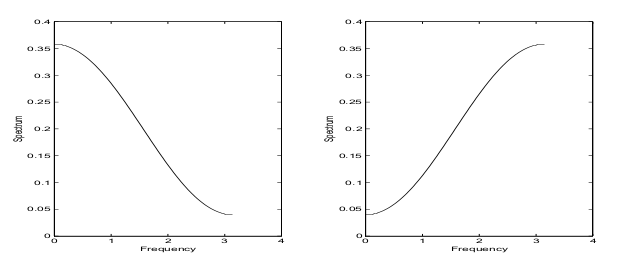
\includegraphics[scale=0.6]{images/spectrumMA1.png}
\caption{Widmo procesu MA(1), dla $\theta = 0.5$ oraz $\theta= -0.5$.} \label{fig-spectrum-ma1}
\end{figure}

Widmo procesu MA(1) możemy obserwować na wykresie \ref{fig-spectrum-ma1}.

\begin{theorem}[Widmo procesu ARMA(p,q)]
Niech $X_t$ będzie procesem stochastycznym opisanym ARMA(p,q), tj
$$
g_\phi(L) x_t = g_\theta(L) \epsilon_t.
$$
Załóżmy, że proces ten jest stacjonarny, czyli wszystkie pierwiastki wielomianu $g_\phi$ leżą w kole jednostkowym. Wtedy widmem procesu $X_t$ jest
$$
S_X (\omega) = \frac{1}{2 \pi} \frac{\abs{g_\theta (e^{-i\omega})}^2}{ \abs{ \function{g_\phi}{ e^{-i \omega} }^2} }\sigma^2_\epsilon.
$$
\end{theorem}

\begin{theorem}[Widmo procesu AR(1)]
Rozważmy $X$ zgodne z procesem AR(1), tj.
$$
X_t = \epsilon_t + \phi X_{t-1}.
$$
Wtedy widmo tego procesu wyraża sie formułą
$$
S_X(\omega) = \frac{1}{2\pi} \bracket{1 + \phi^2 - 2 \phi \cos \omega}^{-1} \sigma_\epsilon^2.
$$
\end{theorem}

\begin{figure}
\centering
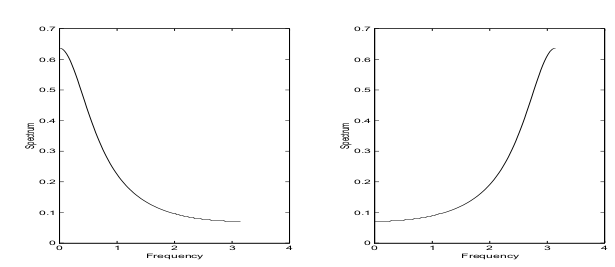
\includegraphics[scale=0.6]{images/spectrumAR1.png}
\caption{Widmo procesu AR(1), dla $\phi = 0.5$ oraz $\phi= -0.5$.} \label{fig-spectrum-ar1}
\end{figure}

Widmo procesu AR(1) możemy obserwować na wykresie \ref{fig-spectrum-ar1}.

\begin{theorem}[O reprezentacji widmowej]
Niech $X_t$ będzie szeregiem czasowym stacjonarnym z zerową wartością oczekiwaną oraz sumowalną w module funkcją autokowariancji. Wtedy istnieją zmienne losowe $\alpha(\omega)$ oraz $\beta(\omega)$ takie, że
$$
x_t = \int_{0}^\pi \bracket{\alpha(\omega) \cos (\omega t) + \beta(\omega) \sin(\omega t) } \dt[\omega].
$$ 
\end{theorem}

\chapter{Prognozowanie wielowymiarowych szeregów czasowych}

Niniejszy rozdział został opracowany na podstawie \citep{kirchgassner2012introduction}. Wyjaśnimy w nim w jaki sposób, z jakich przyczyn i mając jakie cechy szczególne na uwadze - tworzyć będziemy modele predykcyjne oparte o wartości wielu szeregów czasowych. Aby dodatkowo umotywować analizowanie tego rodzajów modeli wymieńmy nagrody imienia Nobla przyznane w tematyce szeregów czasowych.

Nagrody im. Nobla z dziedziny ekonomii 
\begin{itemize}
\item Robert Eagle 2003 / za model ARCH,
\item Clive Granger 2003 / za koncepcje przyczynowości,
\item Christopher Sims 2011 / za model VAR i prace z przyczynowości,
\item Thomas Sargent (2011) / za prace z zakresu przyczynowości.
\end{itemize}

\section{Przyczynowość Grangera}

Podstawę teorii inicjującej tworzenie modeli wielowymiarowych szeregów czasowych dopatruje się dzisiaj w pracy stworzonej i opublikowanej przez Clive'a Grangera w 1969 o tytule "Investigating Causal Relations by Econometric Models and Cross-Spectral Methods". Zanim bowiem porozmawiamy sobie o układach wielowymiarowych szeregów czasowych trzeba wprowadzić sposób określania zależności występujących pomiędzy szeregami w sposób rozumiejący i włączający do warunków:
\begin{itemize}
\item specyfikę świata szeregów czasowych,
\item dobrze oddający relację względem osi czasu, oraz
\item mającym wzmocnione wartości predykcyjne. 
\end{itemize}    
W ujęciu Grangera związki pomiędzy szeregami czasowymi mogą mieć charaketer przyczynowo-skutkowy stąd i cała teoria nazywana jest najczęściej przyczynowością Grangera. Rozważony do tej pory schemat świata wnosił, że wszystkie szeregi czasowe, w sensie procesów stochastycznych, są niezależnymi od siebie, generowanymi przez niezależne szeregi czasowe powstałe z białych szumów. Z punktu widzenia ekonometrycznego - takie przypuszczenie można by nazwać najbardziej wątpliwym założeniem teorii szeregów czasowych. Praktycy bowiem, wręcz skłonni byliby przyjąć zupełnie przyciwstawny punkt orzekający o powszechności występowania związków pomiędzy szeregami czasowymi. 

Kierują nami dwie podstawowe motywacje, które prowadzą do rozważania tego rodzajów związków. 
\begin{itemize}
\item Jeśli pomiędzy szeregami czasowymi występują związki to jest to możliwość do 
\begin{itemize}
\item tworzenia modeli o niższym błędzie prognozy,
\item najbardziej naturalnego tworzenia uogólnień teorii modeli ARIMA.
\end{itemize}
\item Postrzeganie szeregów czasowych we wzajemnych związkach przypomina poszukiwanie zależności regresyjnych. Co do powszechności i łatwości modelowej regresji jesteśmy przekonani - mamy jednak w świadomości, że o ile trywialnym jest wyznaczenie regresji
$$
y_t \sim x_t
$$
o tyle czy do tej pory rozważane modele dopuszczały możliwość regresji z inną chwilą czasu np.
$$
y_t \sim x_{t-1}.
$$
\end{itemize}

\begin{definition}[Informacja]\index{Informacja w sensie Grangera}
Niech $\stochasticprocess{X_t}{t}, \stochasticprocess{Y_t}{t}$ będą dwoma szeregami czasowymi. Niech $x,y$ będą odpowiednio realizacjami tych szeregów czasowych aż do czasu $t$. Definiujemy wtedy 
\begin{description}
\item[Informacją o $X$] nazywamy zdarzenie losowe postaci
$$
\overline{x}_t = \set{ X_t = x_t , X_{t-1} = x_{t-1} , \ldots , X_0 = x_0}, 
$$
\item[Informacją o $Y$] nazywamy zdarzenie losowe postaci
$$
\overline{y}_t = \set{ Y_t = y_t , Y_{t-1} = y_{t-1} , \ldots , Y_0 = y_0}, 
$$
\item[Informacją ] nazwiemy zdarzenie łączące informacje o wartościach wszystkich interesujących nas szeregów czasowych (w tym wypadku dwóch) tj.
$$
I_t = \set{ X_t = x_t, Y_t = y_t , X_{t-1} = x_{t-1}, Y_{t-1} = y_{t-1}, \ldots , X_0 = x_0, Y_0 = y_0}. 
$$
Jeśli szeregi mają różne długości w osi czasu, to informacja zawiera w sobie zawsze całą poprzedzającą wiedzę o ich przebiegu.
\end{description}
\end{definition}

\begin{definition}[Arytmetyka informacji]
Często dla uproszczenia zapisu będziemy stosować notację, który można by nazwać arytmetyką informacji. Niech $x,y,z$ będą trzema szeregami czasowymi oraz niech $I_t$ będzie informacją pochodzącą od $x,y$. Wtedy 
\begin{itemize}
\item Suma informacji $ I_t + \overline{z}_t$ oznacza zdarzenie losowe postaci
$$
\set{ X_t = x_t, Y_t = y_t, Z_t = z_t , X_{t-1} = x_{t-1}, Y_{t-1} = y_{t-1}, Z_{t-1} = z_{t-1}, \ldots , X_0 = x_0, Y_0 = y_0, Z_0 = z_0}. 
$$
\item Różnicą informacji $ I_t - \overline{y}_t$ oznaczać będziemy zdarzenie losowe postaci
$$
\set{ X_t = x_t , X_{t-1} = x_{t-1} , \ldots , X_0 = x_0},
$$
czyli takie w którym cała informacja o $y$ została usunięta.
\end{itemize}
\end{definition}

\begin{definition}[Przyczynowość Grangera]\index{Przyczynowość Grangera}\index{Przyczynowość Grangera!natychmiastowa}
Niech $x_t$ oraz $y_t$ będą szeregami czasowymi - słabo stacjonarnymi. Niech $\sigma^2$ będzie wariancją błędu prognozy $\predict{y}{t}$. 
\begin{itemize}
\item Powiemy, że $x$ jest prostą przyczyną w sensie przyczyności Grangera (jest przyczyną) dla $y$ jeśli 
$$
\sigma^2 ( \predict{y}{t} | I_t ) < \sigma^2 ( \predict{y}{t} | I_t - \overline{x}_t ), 
$$
co onacza, że modele predykcji są lepsze kiedy dostępna jest informacja o wartościach szeregu czasowego $x$.
\item Powiemy, że $x$ jest natychmiastowo przyczynowy dla $y$ jeśli
$$
\sigma^2 ( \predict{y}{t} | I_t + \overline{x}_{t+1} ) < \sigma^2 ( \predict{y}{t} | I_t ), 
$$  
co sprowadza się do opisu, że wartość $y_{t+1}$ może być dokładniej prognozowana gdyby znana była $x_{t+1}$
\item Powiemy, że szeregi $x$ i $y$ są sprzężone zwrotnie jeśli $x$ jest przyczyną dla $y$ oraz $y$ jest przyczyną dla $x$
\end{itemize} 
\end{definition}

\begin{remark}
Sprzężenie zwrotne jest rozumiane tylko w ujęciu prostej przyczynowości. W przypadku natychmiastowej przyczynowości ma zastosowanie Twierdzenie \ref{theorem-instant-casuality}. Mówienie o jednostonnej przyczynowości natychmiastowej jest rozumiane jako informacja o tej przyczynowości wraz z informacją a priori o kierunku tej zależności. Tzn. że jeśli dla przyczynowości natychmiastowej deklarujemy jakiś kierunek - to decydują o tym jedynie zależności poza matematyczne.
\end{remark}

\begin{theorem}[{\citep[Twierdzenie 3.1]{kirchgassner2012introduction}}]\label{theorem-instant-casuality}
$x$ jest natychmiastową przyczyną dla $y$ wtedy i tylko wtedy gdy $y$ jest natychmiastową przyczyną dla $x$.
\end{theorem}

\begin{definition}[Notacja dla przyczynowości]
Zgodnie z omówionymi powyżej pojęciami oznacza to możliwości następujących zależności, które będą oznaczane wg podanych poniżej symboli
\begin{itemize}
\item Szeregi $x$ i $y$ mogą być niezależne $(x,y)$,
\item Szeregi $x$ i $y$ są natychmiastowo zależne, ale nie są zależne w sposób prosty $(x \sim y)$ (regresja).
\item $x$ jest przyczyną dla $y$, ale bez natychmiastowości $(x \rightarrow y)$,
\item $y$ jest przyczyną dla $x$, ale bez natychmiastosości $(x \leftarrow y)$,
\item $x$ jest przyczyną dla $y$, występuje natychmiastość $( x \Rightarrow y)$,
\item $y$ jest przyczyną dla $x$, występuje natychmiastość $( x \Leftarrow y)$,
\item $x$ i $y$ są w sprzężeniu zwrotnym, bez natychmiastowości $(x \leftrightarrow y)$,
\item $x$ i $y$ są w sprzężeniu zwrotnym, występuje natychmiastość $(x \Leftrightarrow y)$.
\end{itemize}
\end{definition}

\subsection{Autoregresja dwuzmiennowa}

W dalszej części wprowadźmy model autoregresji dwuzmiennowej. Potrzebujemy następującego pojęcia

\begin{definition}[Macierz wielomianowa]\index{Macierz wielomianowa}
Macierzą wielomianową nazywamy wielomian, którego współczynnikami są macierze zgodnego wymiaru.
\end{definition}

Przypomijmy, że mając jeden szereg czasowy $x$ można było zapisać równanie autoregresji pisząć 
$$
A(L) x_t  = u_t,
$$ 
gdzie $A(\cdot)$ było pewnym wielomianem (z reguły z $1$ w miejscu wyrazu wolnego), $L$ oznaczało operator opóźnienia a $u_t$ było procesem stochastycznym w typie białego szumu. W przypadku dwóch zmiennych równanie przybierze postać:

\begin{definition}[Model autoregresji dwuzmiennowej]\index{Model!autoregresji dwuzmiennowej}
Niech $x,y$ będą dwoma słabo stacjonarnymi szeregami czasowymi, niech $A$ będzie macierzą wielomianową postaci
$$
A(\cdot) = \begin{bmatrix}
\alpha_{11} (\cdot) & \alpha_{12} (\cdot)\\
\alpha_{21} (\cdot) & \alpha_{22} (\cdot)
\end{bmatrix}.
$$
Wtedy modelem autoregresji dwuzmiennowej nazywamy równanie postaci
$$
A(L) \begin{bmatrix}
y_t\\ x_t
\end{bmatrix} = \begin{bmatrix}
u_t \\ v_t
\end{bmatrix},
$$
lub równoważnie
$$
\begin{bmatrix}
\alpha_{11} (L) & \alpha_{12} (L)\\
\alpha_{21} (L) & \alpha_{22} (L)
\end{bmatrix} \begin{bmatrix}
y_t\\ x_t
\end{bmatrix} = \begin{bmatrix}
u_t \\ v_t
\end{bmatrix},
$$
gdzie $u_t, v_t$ są realizacjami szumu białego. Ponadto zakładamy, że równanie to jest w postaci znormalizowanej i zredukowanej tzn.
\begin{align*}
& \alpha_{11}^0 = \alpha_{22}^0 = 1,\\
& \alpha_{12}^0 = \alpha_{21}^0 = 0.
\end{align*}
\end{definition}

\begin{remark}
Zauważmy, że jeśli w powyższym modelu mamy zmienność natychmiastową to oznacza to, że szeregi czasowe $u_t$ oraz $v_t$ nie są niezależne. 
\end{remark}

\begin{theorem}[O reprezentacji przyczynowości]
Niech $x,y$ będą opisane przez model autoregresji dwuzmiennowej. Wtedy prawdziwa jest następująca charakteryzacja
\begin{itemize}
\item $ (x,y) \lor (x-y)$ gddy $\alpha_{12}(L) \equiv \alpha_{21}(L) \equiv 0$.
\item $ (x \rightarrow y) \lor (x \Rightarrow y)$ gddy $ \lnot \alpha_{12}(L) \equiv 0 \land \alpha_{21}(L) \equiv 0$. 
\item $ (x \leftarrow y) \lor (x \Leftarrow y)$ gddy $  \alpha_{12}(L) \equiv 0 \land \lnot \alpha_{21}(L) \equiv 0$.
\item $ (x \leftrightarrow y) \lor (x \Leftrightarrow y)$ gddy $ \lnot \alpha_{12}(L) \equiv 0 \land \lnot \alpha_{21}(L) \equiv 0$.
\end{itemize}
\end{theorem}

\subsection{Dwuzmiennowa średnia krocząca}

W podobny analogiczny sposób możemy wprowadzić model średniej kroczącej

\begin{definition}[Model dwuzmiennowej średniej kroczącej]\index{Model!dwuzmiennowy MA(q)}
Niech $x,y$ będą dwoma słabo stacjonarnymi szeregami czasowymi, niech $B$ będzie macierzą wielomianową postaci \footnote{lub ogólniej - macierzowym szeregiem potęgowym}
$$
B(\cdot) = \begin{bmatrix}
\beta_{11} (\cdot) & \beta_{12} (\cdot)\\
\beta_{21} (\cdot) & \beta_{22} (\cdot)
\end{bmatrix}.
$$
Wtedy modelem dwuzmiennowej średniej kroczącej nazywamy równanie postaci
$$
\begin{bmatrix}
y_t\\ x_t
\end{bmatrix} = B(L) \begin{bmatrix}
u_t \\ v_t
\end{bmatrix},
$$
lub równoważnie
$$
 \begin{bmatrix}
y_t\\ x_t
\end{bmatrix} = \begin{bmatrix}
\beta_{11} (L) & \beta_{12} (L)\\
\beta_{21} (L) & \beta_{22} (L)
\end{bmatrix} \begin{bmatrix}
u_t \\ v_t
\end{bmatrix},
$$
gdzie $u_t, v_t$ są realizacjami szumu białego. Ponadto zakładamy, że równanie to jest w postaci znormalizowanej i zredukowanej tzn.
\begin{align*}
& \beta_{11}^0 = \beta_{22}^0 = 1,\\
& \beta_{12}^0 = \beta_{21}^0 = 0.
\end{align*}
\end{definition}

\begin{theorem}[O reprezentacji przyczynowości]
Niech $x,y$ będą opisane przez model dwuzmiennowej średniej kroczącej. Wtedy prawdziwa jest następująca charakteryzacja
\begin{itemize}
\item $ (x,y) \lor (x-y)$ gddy $\beta_{12}(L) \equiv \beta_{21}(L) \equiv 0$.
\item $ (x \rightarrow y) \lor (x \Rightarrow y)$ gddy $ \lnot \beta_{12}(L) \equiv 0 \land \beta_{21}(L) \equiv 0$. 
\item $ (x \leftarrow y) \lor (x \Leftarrow y)$ gddy $  \beta_{12}(L) \equiv 0 \land \lnot \beta_{21}(L) \equiv 0$.
\item $ (x \leftrightarrow y) \lor (x \Leftrightarrow y)$ gddy $ \lnot \beta_{12}(L) \equiv 0 \land \lnot \beta_{21}(L) \equiv 0$.
\end{itemize}
\end{theorem}

\subsection{Testy do badania przyczynowości}

Do badania zjawisk przyczynowości Grangera dostępne jest kilka testów.

\begin{itemize}
\item Direct Granger Procedure (bezpośredni test Grangera) opracowany przez Thomasa Sargenta,\index{Test!bezpośredni Grangera}
\item Test Haugh-Pierce, \index{Test! Haugh-Pierce}
\item Test Hsiao.\index{Test Hsiao}
\end{itemize}

\section{Model wielowymiarowy VAR}

Naturalną konsekwencją występowania zależności pomiędzy szeregami czasowymi jest tworzenie ich modeli łącznych czyli wielowymiarowych. Pokazaliśmy wytworzony w tym rozumieniu model dwóch zmiennych jak również ogólny zarys jak można by rozwijać modele w kierunku większej ilości wymiarów. Dalszym zadaniem jest w takim razie ustalenie w jaki sposób najlepiej rozszerzać te modele aby prezentowały możliwie jak najlepiej zwarte i opisane teorie. W tej części omówimy tutaj teorię opracowaną przez Christophera Simsa i zaprezentowaną w 1980 roku. Sims był jednym ze zwolenników przyczynowości Grangera i rozwinął jego teorię tworząc koncepcję wektorów procesów autoregresywnych. 

\subsection{Odrzucenie modelu niepełnych zależności}

Akceptując model przyczynowości Grangera można dojść do wniosku, że wystarczy odszukać wszystkie statystycznie istotnie przyczynowości ażeby zaproponować jeden spójny model zjawiska. Przeciwną tezę popularyzował właśnie Sims, w której wszystkie możliwe konfiguracje zależności są dostępne. Za głównym argumentem przemawiającym za taką tezą Sims wymieniał to że modele powinny wykazywać się racjonalnością skoro modelują zjawiska uwzględniające ludzkie rozumowanie. Sims podał następujący przykład na poparcie.

\begin{example}
Rozważmy zmieniającą się cenę rynkową kawy, która jak w każdym modelu jest wypadkową popytu i podaży. Poziom tej ceny jest głównie zależny od poziomu jej produkcji w Brazylii, gdzie w porze jesiennej odbywają się zbiory na platacjach kawy. Rozważmy, że w danym roku pojawiły się silne przymrozki wiosną, którę dotknęły platacje kawy. W efekcie czego spodziewane przyszłe zbiory w znaczącym stopniu mogły ucierpieć. W sposób oczywisty będzie to wpływało na wartość podaży na kawę, więc w modelu przyczynowym odnotowano by wzrost ceny kawy na jesieni na skutek zmniejszonych plonów. Tak sytuację zinterpretowałby model uwzględniający niepełne zależności. Odrzucono bowiem możliwość wpływu pogody w Brazylii na popyt na kawę. Rozszerzając model przyczynowy o elementy racjonalności postępowania zauważamy, że osoby (głównie duży nabywcy) wobec informacji o problemach na platacjach kawy w Brazylii decydują się zakupić większe ilości w obawie o wzrost cen. W efekcie uzyskujemy niespodziewany efekt przyczynowy pomiędzy pogodą na platacjach w Brazylii a siłą nabywczą na kawę. 
\end{example} 
Przykład ten ilustruje sytuację w której model zjawiska wielowymiarowego jest czymś innym niż suma kilku prostszych modeli (produkcja plantacji zależna od pogody, podaż zależna od produkcji w Brazylii, popyt zależny jedynie od innych czynników).

Według Simsa złym sposobem rozumienia modeli wielowymiarowych było badanie jedynie silnych związków przyczynowych i jeśli chcemy zaproponować odpowiedzialny model - powinniśmy rozpocząć od dopuszczenia wszelakich związków pomiędzy zmiennymi na początku konstruowania modelu. Oparty o to przesłanie model Sims nazwał modelem VAR - Vector AutoRegression systems, w którym dopuszczalne są wszystkie zależności autoregresyjne pomiędzy zmiennymi aż do określonej głębi czasu.

Uwaga! Z uwagi na rozważanie tu wektorów szeregów czasowych - znacząco trudniej będzie rozróżnić wektorowy proces stochastyczny od jego realizacji. Dodatkowo miejmy na uwadze, że wszystkie mnożenia macierzowe traktują wektory domyślnie jak wektory kolumnowe (klasyczna notacja).



\subsection{Definicja modelu Var(p)}

Analizę modelu VAR rozpocznijmy od ich definicji.

\begin{definition}[Model Var(p)] \index{Model!VAR(p)}
Niech $\stochasticprocess{X_t}{t}$ będzie $k-$wymiarowym procesem stochastycznym. Powiemy, że proces ten jest zgodny z modelem Var(p), jeśli opisany jest równaniem
$$
X_t = \sigma + A_1 X_{t-1} + A_2 X_{t-2} + \ldots + A_p X_{t-p} + U_t,
$$
gdzie $A_i$ są macierzami kwadratowymi o wymiarach $k \times k$, $\sigma$ jest stałym wektorem a $U_t$ jest wektorem procesów w typie białego szumu. 
\end{definition}

\begin{remark}
Równanie modelu Var(p) może być również zapisane w zwartej postaci
$$
A(L) X_t = \sigma + U_t,
$$
gdzie 
$$
A(L) = I_k - A_1 L - A_2 L^2 - \ldots - A_p L^p,
$$
z $L$ oznaczającym operator opóźnienia. 
\end{remark}

\begin{remark}[Własności wektora zaburzeń $U_t$]

Żeby lepiej zrozumieć działanie $U_t$ przyjrzyjmy się jego własnościom (naszym oczekiwaniom co do jego własności).
\begin{itemize}
\item $\Ex{U_t} = 0$ oczywiście rozumianym w sensie zera k-wymiarowego. 
\item $\Ex{U_t U_t^T} = \sigma_{uu}$ niezerowa macierz kowariancji, czyli poszczególne składowe zaburzeń mogą być zależne ze sobą, (ale)
\item $\Ex{U_t U_s^T} = 0 $ dla dowolnego $s \neq t$ - zatem zaburzenia mogą być wzajemnie zależne - ale tylko dla wspólnej chwili czasu.
\end{itemize}
Pamiętamy nieustannie, że zależności pomiędzy $u_t[i]$ i $u_t[j]$ są tłumaczone wprost na natychmiastowe zależności pomiędzy $i-$tą i $j-$tą współrzędną wektora $X_t$. 
\end{remark}

\begin{theorem}
Jeśli $\stochasticprocess{X_t}{t}$ jest opisane modelem Var(p). Wtedy model jest stacjonarny (słabo) wtedy i tylko wtedy, gdy wszystkie pierwiastki równania charakterystycznego leżą poza kołem jednostkowym tj.
$$
\det \bracket{I_k - A_1 z - A_2 z^2 - \ldots - A_p z^p} \neq 0, \text{ dla } \abs{z} \leq 1.
$$
\end{theorem}

\begin{theorem}[Postać MA modelu Var(p)]
Jeśli $\stochasticprocess{X_t}{t}$ jest opisane modelem Var(p) i jest to proces stacjonarny (słabo) to wtedy równanie
$$
A(L) X_t = \sigma + U_t,
$$
można zapisać w równoważnej postaci 
$$
X_t = \mu + B(L) U_t,
$$
gdzie $B(L) = A^{-1}(L) = I_k - \sum_{j=1}^{\infty} B_j L^j$, nazywanej postacią MA procesu Var(p).
\end{theorem}

\begin{definition}[Macierz autokowariancji]\index{Macierz!autokowariancji}
Niech $\stochasticprocess{X_t}{t}$ będzie procesem opisanym modelem Var(p). Wtedy macierzą autokowariancji nazywamy macierz $\Gamma_X(\tau)$ równą
$$
\Gamma_X(\tau) = \Ex{ (X_t - \mu) \cdot (X_{t-\tau} - \mu)^T}.
$$ 
\end{definition}

Możemy bez straty ogólności przyjąć $\mu = 0$. Wtedy
\begin{align*}
\Ex{X_t X_{t-\tau}^T} & = A_1 \Ex{X_{t-1} X_{t-\tau}^T} + A_2 \Ex{X_{t-2} X_{t-\tau}^T} + \ldots + A_p \Ex{X_{t-p} X_{t-\tau}^T} + \Ex{U_t X_{t-\tau}^T}.
\end{align*}
Prowadzi to do układów równości
\begin{align*}
\Gamma_X(\tau) &= A_1 \Gamma_X(\tau-1) + A_2 \Gamma_X(\tau - 2) + \ldots + A_p \Gamma_X(\tau - p), \\
\vdots & \vdots \\
\Gamma_X(0) &= A_1 \Gamma_X(-1) + A_2 \Gamma_X(- 2) + \ldots + A_p \Gamma_X(- p) + \Sigma_{uu}.
\end{align*}
Korzystając z tego, że $ \gamma_{ij}(-k) = \gamma_{ji}(k)$ otrzymujemy, że $\Gamma_X(-k) = \Gamma_X(k)^T$. Dzięki czemu otrzymujemy układ liniowy $\tau+1$ równań z $\tau+1$ niewiadomymi. Jeśli uda się nam go rozwiązać otrzymamy pełną postać funkcji macierzy autokowariancji (wartościami funkcji autokowariancji są macierze). 

\begin{definition}[Macierz autokorelacji]\index{Macierz!autokorelacji}\index{Macierz!ACF}
Macierzą korelacji dla procesu $\stochasticprocess{X_t}{t}$ zgodnego z modelem Var(p) nazywamy macierz o tych samych wymiarach co macierz autokowariancji $\Gamma_X(\tau)$ z wartościami opisanymi wzorem
$$
\rho_{ij}(\tau) = \frac{\gamma_{ij}(\tau)}{ \sqrt{\gamma_{ii}(0) \gamma_{jj}(0) } }, i,j = 1, \ldots, k.
$$
Alternatywnie wykorzystując następującą macierz $D^{-1}$ równą
$$
D^{-1} = \begin{bmatrix}
\frac{1}{\sqrt{\gamma_{11}(0)}} & 0 & \cdots & 0 \\
0 & \frac{1}{\sqrt{\gamma_{22}(0)}} & \cdots & 0 \\
\vdots & \vdots & \ddots & \vdots \\
0 & 0 & \cdots & \frac{1}{\sqrt{\gamma_{kk}(0)}}
\end{bmatrix},
$$
możemy to uprościć do zapisu
$$
R_X(\tau) = D^{-1} \Gamma_X(\tau) D^{-1}. 
$$
\end{definition}

Do predykcji wykorzystywany jest estymator postaci
$$
\predict{X}{t} = \Ex{X_{t+1} } = \sigma + A_1 X_t + A_2 X_{t-1} + \ldots + A_p X_{t-p+1}. 
$$

\begin{remark}
Przy założeniu stacjonarności dysponując dwiema postaciami szeregu czasowego 
\begin{itemize}
\item Wykorzystujemy postać autoregresyjną do predykcji wartości, natomiast
\item postać średniej kroczącej do estymacji błędów i innych analiz.
\end{itemize}
\end{remark}

Do ocenu modelu możemy wykorzystać kilka miar błędów
\begin{itemize}
\item Błąd końcowej predykcji\footnote{Final Prediction Error} postaci \index{Błąd!końcowej predykcji}\index{Błąd!FPE}
$$
FPE(p) = \bracket{\frac{T+kp+1}{T-kp-1}}^k \det \Sigma(p).
$$
\item Kryterium Akaike (AIC)\index{Błąd!AIC}
$$
AIC(p) = \function[{\ln}]{\det \Sigma(p)} + (k + pk^2) \frac{2}{T}.
$$
\item Kryterium Hannan-Quinn (HQ) \index{Błąd!HQ}\index{Błąd!Hannan-Quinn}
$$
HQ(p) = \function[{\ln}]{\det \Sigma(p)} + (k + pk^2) \frac{2 \function[{\ln}]{\function[{\ln}]{T} } }{T}.
$$
\item Kryterium Schwarza (SC) \index{Błąd!Schwarza}\index{Błąd!SC}
$$
SC(p) = \function[{\ln}]{\det \Sigma(p)} + (k + pk^2) \frac{\function[{\ln}]{T} }{T} .
$$
\end{itemize}
W powyższych wzorach $p$ to rozmiar modelu, $k$ to ilość zmiennych, $T$ rozmiar zbioru danych. Natomiast $\Sigma(p)$ oznacza macierz kowariancji błędów, tj.
$$
\Sigma(p) = \frac{1}{T} \sum_{t=1}^{T} \epsilon_t \epsilon_t^T.
$$

Podstawowym problemem modelu Var(p) jest olbrzymia ilość parametrów ( $k$ ilość zmiennych, $p$ ilość składowych autoregresyjnych - daje nam liczbę parametrów rzędu $ k^2 \cdot p$). Przykład Simsa pokazuje, że tworząc model nie wolno z góry założyć pewnych relacji. Jednak już nauczone modele pokazują, że znacząca część parametrów posiada wartości nieistotnie różne od zera i mogą one zostać usunięte z modelu. Zatem,  aby zoptymalizować model, można go uprościć z końcowo nieistotnych przyczynowości.

\subsection{Model Var a przyczynowość Grangera}

O przyczynowości Grangera powiedziane zostało już dużo i możemy to jedynie rozszerzyć o pewne nieoczywiste interpretacje. Niech $\stochasticprocess{X_t}{t}$ będzie zgodny z modelem Var(p) o $k$ zmiennych. Z dokładnością do kolejności tych zmiennych możemy dokonać dekompozycji naszego problemu do $k_1$ pierwszych zmiennych oraz pozostałych w liczbie $k_2$ tj. $k_1 + k_2 = k$. Wtedy również można by utworzyć modele Var(p) dla pierwszych $k_1$ zmiennych oraz pozostałych $k_2$ zmiennych z osobna. Posługując się $X_{1,t}$ jako oznaczenie $k_1$ pierwszych wierszy danych z $X_t$ oraz $X_{2,t}$ dla pozostałych wierszy $X_{t}$. Wtedy (pomimo, że nasze składowe będą macierzami lub wektorami) napisać możemy łączny model Var(p) jako
$$
\begin{bmatrix}
A_{11}(L) & A_{12}(L) \\
A_{21}(L) & A_{22}(L) 
\end{bmatrix}
\begin{bmatrix}
X_{1,t} \\
X_{2,t}
\end{bmatrix} = \begin{bmatrix}
\sigma_1 \\
\sigma_2
\end{bmatrix} + 
\begin{bmatrix}
U_{1,t} \\
U_{2,t}
\end{bmatrix}.
$$

Wtedy, korzystając ze wszystkich tych modeli Var(p), możemy tak jak dla pojedynczych wartości obliczyć współczynniki wielomianów $A_{12}$ $A_{21}$ aby stwierdzić obecność przyczynowości Grangera w naszym modelu. 

Zdecydowanie trudniej jest uzyskać informacje o natychmiastowej przyczynowości. Wynika to z zależności podefiniowanych w procesach szumu białego. Do przeprowadzenia tej analizy przechodzimy do postaci pomocniczej po wykonaniu dekompozycji Choleskiego macierzy kowariancji $\Sigma_{uu}$.

\begin{definition}[Rozkład Choleskiego]\index{Rozkład Choleskiego}
Jeśli macierz $A$ jest symetryczną i dodatnio określoną to istnieje macierz $L$ dolna trójkątna taka, że
$$
A = L L^T.
$$
\end{definition}

Załóżmy, że macierz kowariancji została poddana rozkładowi Choleskiego, i zatem
$$
\Sigma_{uu} = P P^T. 
$$
Dokonamy przekształcenia równania Var(p) dla jest postaci średniej kroczącej
\begin{align*}
X_t &= \mu + U_t - \sum_{j=1}^{\infty} B_j U_{t-j} \\
X_t &= \mu + P P^{-1} U_t - \sum_{j=1}^{\infty} B_j P P^{-1} U_{t-j} \\
&= \mu + P W_t - \sum_{j=1}^{\infty} \theta_j W_{t-j} \\
&= \mu + \theta(L) W_t,
\end{align*}
gdzie $\theta_j = B_j P$, $\theta(0) = P$, $W_t = P^{-1} U_t$ i uzyskujemy, że 
$$
\Sigma_{ww} = P^{-1} \Sigma_{uu} \bracket{P^{T}}^{-1} = P^{-1} P P^T \bracket{P^{T}}^{-1} = I_k
$$

Proces $W_t$ nazywa się wektorem innowacji. Jest to wektor nieskorelowany, inaczej niż wektor zaburzeń $U_t$. 
W ujęciu tej transformacji nasze równanie przekształca się do 
$$
X_t = \begin{bmatrix}
X_{1,t} \\
X_{2,t}
\end{bmatrix} = 
\begin{bmatrix}
\mu_1 \\
\mu_2
\end{bmatrix} + \begin{bmatrix}
\theta^0_{11} & 0 \\
\theta^0_{21} & \theta^0_{22}
\end{bmatrix}
\begin{bmatrix}
W_{1,t} \\
W_{2,t}
\end{bmatrix} - \begin{bmatrix}
\theta^1_{11} & \theta^1_{12} \\
\theta^1_{21} & \theta^1_{22}
\end{bmatrix} \begin{bmatrix}
W_{1,t-1} \\
W_{2,t-1}
\end{bmatrix} - \ldots .
$$

W tym ujęciu wystarczy zbadać czy wartość parametru $\theta^0_{21} $ jest równa zero,  aby orzec o braku natychmiastowości. Należy mieć świadomość tego, że podjęta transformacja definiuje w swoim wnętrzu kierunek natychmiastowości - więc może on być ostatecznie rozpoznany w sposób niezgodny z intuicją.

\subsection{Analiza impuls - odpowiedź} \index{Analiza impuls-odpowiedź}

Innym sposobem na analizę występujących zależności pomiędzy zmiennymi a poprzez to eliminację nieistotnych zmiennych jest analiza impuls - odpowiedź. Analizę tę można stosować zarówno do postaci średniej kroczącej jak i do postaci z innowacjami. 

\begin{definition}[Analiza impuls - odpowiedź]
Przez analizę impuls - odpowiedź rozumiemy obserwowanie zależności pomiędzy składowymi wektora procesu autoregresyjnego poprzez porównanie właściwego modelu predykcyjnego oraz modelu w którym do ustalonej zmiennej $u_j$ / $w_j$ w ustalonej chwili czasu $t$ wprowadzona zostaje zmodyfikowana wartość poprzez dodanie/odjęcie do niej wartości odchylenia standardowego - i obserwowanie różnic generowanych w późniejszych chwilach czasu $t+1, t+2, \ldots$ we wszystkich zmiennych $x_i$. 
\end{definition}

\chapter{Modelowanie szeregów niestacjonarnych}\label{chapter-szeregi-niestacjonarne}

Poniższy rozdział został przygotowany w oparciu o \citep[Rozdział 5]{kirchgassner2012introduction}.

Ostatnią część niniejszego wykładu poświęcimy modelowaniu szeregów niestacjonarnych. Co prawda do tej pory omówione zostały dwie metody postępowania już z takimi szeregami. 
\begin{itemize}
\item Odjęcie regresji - w pierwszym przypadku spodziewamy się, że trend i procesy losowane wpływają na siebie w sposób addytywny, estymujemy więc składową trendu z wykorzystaniem regresji, a pozostałą cześć próbujemy estymować z wykorzystaniem teorii stacjonarnych szeregów czasowych.
\item Drugą z metod jest badanie szeregu przyrostów - podejście, które stanowi jeden z fundamentów modeli ARIMA.
\end{itemize}
Obydwa z wymienionych podejść współdzielą jedną i tę samą wadę. Absolutnie wykluczają interakcje pomiędzy składowymi trendu a losowością. Przyjrzyjmy się w dalszej części teorii, która stara się opisać również inne postępowanie z szeregami niestacjonarnymi.

\section{Rodzaje niestacjonarności}

Podstawowym założeniem dotyczącym stacjonarności szeregu jest stałość wartości oczekiwanej w czasie. Naturalnym będzie zatem rozpoczęcie analizowania szeregów niestacjonarnych od realizacji naruszających to właśnie założenie. 
Omówimy dwie podgrupy szeregów niestacjonarnych o zmiennej wartości oczekiwanej naruszających to założenie:
\begin{itemize}
\item te gdzie trend zależy od czasu w sposób deterministyczny,
\item oraz te gdzie trend zależy od czasu w sposób stochastyczny.
\end{itemize}

Rozpocznijmy naszą analizę od pierwszego z rodzajów.

\subsection{Szeregi z trendem deterministycznym}

Operując podstawową teorią z zakresu matematyki wiemy, że jeśli nasz szereg czasowy posiada w sposób niejawny opisaną wartość to możemy ją opisać lub chociażby przybliżyć za pomocą pewnego wielomianu. 

\begin{remark}
Niech $x_t$ będzie szeregiem czasowym stacjonarnym i odwracalnym zgodnym z modelem ARMA(p,q) o średniej równej 0. Wtedy szereg $y_t$ opisany zależnością 
$$
y_t = \sum_{i=0}^{m} \delta_i t^i + x_t,
$$
jest szeregiem niestacjonarnym z trendem zależnym deterministycznie\index{Szereg!czasowy!z deterministycznym trendem}. 

Łatwo zaobserwować, że 
$$
\Ex{y_t} = \sum_{i=0}^{m} \delta_i t^i = \mu_t,
$$
gdzie $mu_t$ opisuje w takim układzie wartość oczekiwaną zmieniającą się w czasie. W zakresie autokorelacji obserwujemy
$$
\Ex{ (y_t - \mu_t) (y_{t+\tau} - \mu_{t+\tau})} = \Ex{x_t x_{t+\tau}} = \gamma_X(\tau).
$$
\end{remark}

Powyższy model jest wskazany do stosowania gdzie obserwowana wartość oczekiwana zmienia się w sposób deterministyczny, ale i tylko tam gdzie wariancja jest stała w przebiegu realizacji szeregu czasowego.

\begin{remark}
Rozważmy proces zgodny z modelem $AR(1)$ opisany równaniem
$$
y_t = \alpha y_{t-1} + u_t,
$$
z $\alpha > 1$. Wtedy tak zdefiniowany proces nie jest stacjonarny gdyż
$$
y_t = y_0 \alpha^t + \sum_{i=0}^{t-1} \alpha^{i-1} u_{t-i},
$$ 
i w efekcie czego:
$$
\Ex{y_t} = \alpha^t \Ex{y_0},
$$
co przy $t \to \infty$ powoduje wykładniczą rozbieżność wartości oczekiwanej do nieskończoności. W zakresie wariancji tego procesu otrzymujemy
$$
\Variance{y_t} = \bracket{1+\alpha^2+\alpha^4+\ldots+\alpha^{2(t-1)}} \sigma^2_u = \frac{1-\alpha^{2t}}{1-\alpha^2	} \sigma^2_u.
$$
Zatem również wariancja w tym procesie wzrasta wykładniczo. 
\end{remark}

\subsection{Szeregi z trendem stochastycznym}

Poprzednia część zakończyła się rozważeniem modelu szeregu czasowego zgodne z AR(1), ale z parametrem zapewniającym wykładniczą rozbieżność zarówno wartości oczekiwanej jak wariancji.
W ten sposób obserwujemy następującą trychotomię
\begin{itemize}
\item gdy $\abs{\alpha} < 1$ proces AR(1) jest stacjonarny,
\item gdy $\abs{\alpha} > 1$ proces AR(1) jest niestacjonarny z trendem deterministycznym,
\item ostatni przypadek omówimy teraz szerzej gdyż będą to błądzenia losowe. 
\end{itemize}

Rozważmy podstawowy proces błądzenia losowego opartego o AR(1) tj. opartego o równanie
$$
y_t = y_{t-1} + u_t
$$

Proces działający w ten sposób nie jest oczywiście stacjonarny. Co prawda:
$$
\Ex{y_t} = \Ex{y_0} = const,
$$
ale
$$
\Variance{y_t} = \sum_{i=1}^{t} u_t = t \sigma^2_u.
$$

Rozszerzmy koncepcje oparte o błądzenie losowe\index{Błądzenie losowe}. Aby móc zastosować tę koncepcję - błądzenie losowego musiałoby posiadać trend. Wykorzystamy proces nazywany błądzeniem losowym z ślizgiem\index{Błądzenie losowe z ślizgem}. Uzyskujemy efekt ślizgu poprzez dodanie stałej składowej w równaniu, tj. 
$$
y_t = \delta + y_{t-1} + u_t
$$
Wtedy nasz proces pozostaje niestacjonarny mając za swoje charakterystyki
\begin{align*}
& \Ex{y_t}= y_0 + \delta t = \mu_t, \\
& \Variance{y_t} = \delta t , \\
& \Covariance{y_t}{y_{t-\tau}}= (t-\tau) \sigma^2, \\
& \function[{\rho_X}]{\tau,t} = \sqrt{1 - \frac{\tau}{t}}.
\end{align*}

\begin{figure}
\centering
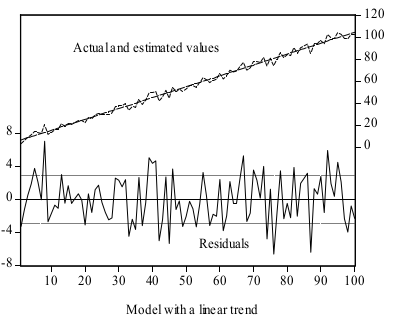
\includegraphics[scale=1]{images/deterministic_trend_residuas.png}
\caption{Trend deterministyczny}
\label{figure-deterministic-trend}
\end{figure}

\begin{figure}
\centering
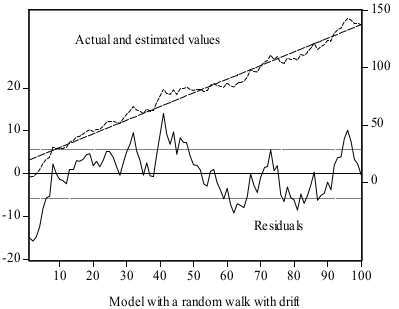
\includegraphics[scale=1]{images/stochastic_trend_residuas.png}
\caption{Trend stochastyczny}
\label{figure-stochastic-trend}
\end{figure}

Sposób w jaki jeden z rodzajów trendów wyróżnia się wobec drugiego widać wyraźnie na wykresach
\ref{figure-deterministic-trend} oraz \ref{figure-stochastic-trend}. Dwa modele w praktycznych podejściach rozpoznaje się poprzez rezydua z modelu. Model deterministyczny pozostawia rezydual w typie szumu białego, a model stochastyczny w innej zależności.

Różnice widać również z całości przebiegu. W wersji ze trendem deterministycznym, znajomość chwili czasu jest dostateczna do określenia wartości średniej w prognozie na kolejny moment czasu. W modelach stochastycznych wartość ta jest silnie zależna od bieżącego stanu realizacji szeregu czasowego.

Wprowadźmy dalej proste uogólnienie błądzenia losowego z ślizgiem. 

\begin{remark}
Niech $x_t$ będzie szeregiem czasowym stacjonarnym zgodnym z ARMA(p,q). Rozważamy szereg czasowy $y_t$ opisany wzorem
$$
y_t = \delta + y_{t-1} + x_t.
$$
Szereg opisany takim modelem nazywany jest różnicowo - stacjonarnym, gdyż $w_t = y_t - y_{t-1}$ jest stacjonarny
\end{remark}

\begin{definition}[Szereg czasowy całkowalny rzędu $d$]\index{Szereg!czasowy!całkowalny rzędu $d$}
Szereg czasowy nazywamy całkowalnym rzędu $d$ jeśli istnieje stacjorany szereg czasowy $x_t$ taki, że jest równy $d$-tej różnicy szeregu $y_t$, tzn.
$$
(1-L)^d y_t = \sigma + x_t.
$$
Procesy z tej rodziany oznaczane są przez $I(d)$. Jeśli proces $x_t$ jest zgodny z ARMA(p,q), to jest on procesem z rodziny ARIMA(p,d,q). Z uwagi na postać wielomianu nie jest on stacjonarny, gdyż $\alpha(L)$ ma $d$-pierwiastów, wszystkie o module równym $1$.  
\end{definition}

\section{Testy jednostkowe pierwiastków}

Istotnym w ujęciu poprzedniej części jest określenie charakterystyki opisującej daną konkretną niestacjonarność. Podstawowa z metod orzekająca aby przeglądać kolejne szeregi różnic, nie posiada jasnych kryteriów, którą kolejną różnice wskazać za podstawową. Z uwagi na to przyjrzymy się metodom, która wspierają analityków z zakresu ocenienia rzędu $d$ - zbiorczo nazywanymi testami jednostkowymi pierwiastków.

Występują tutaj 3 różne podstawowe testy
\begin{itemize}
\item Test Dickey'a - Fullera, w którym przypuszczamy, że nasz szereg pochodzi z modelu AR(1). Hipoteza zerowa orzeka, że jest to proces błądzenia losowego, wobec alternatywy, że jest on procesem stacjonarnym. \index{Test!Dickey'a-Fullera}
\item Ulepszony test Dickey'a - Fullera (ADF), który zakłada model AR(p). \index{Test!ADF}
\item Test Phillips-Perron - w kórym włączone są jeszcze elementy heterosekdastyczności.  \index{Test!Phillipsa-Perrona}
\end{itemize}

\section{Dekompozycje szeregów niestacjonarnych}

Innymi jeszcze metodami stosowanymi do modelowania szeregów niestacjonarnych są próby ich dekompozycji. W ogólnym zarysie poszukują one dekompozycji szeregu czasowego w myśl wzoru
$$
y_t = y_t^p + y_t^t,
$$
gdzie $y_t$ jest szeregiem niestacjonarnym, $y_t^p$ jest składową niestacjonarną - najczęściej błądzeniem losowym, a $y_t^t$ jest składową stacjonarną. Przykładem wyników w tej teorii jest na przykłąd następujące twierdzenie

\begin{theorem}[{Twierdzenie Beveridge - Nelson (1981)\citep[{Sekcja 5.4}]{kirchgassner2012introduction}}]\index{Twierdzenie!Beveridge-Nelson}
Każdy proces zgodny z modelem $ARIMA(p,1,q)$ można rozłożyć na dwie składowe z których 
\begin{itemize}
\item Pierwsza jest błądzeniem losowym ze ślizgiem,
\item Druga jest szeregiem czasowym stacjonarnym.
\end{itemize}
\end{theorem}

\chapter{Inne modele prognostyczne}

Rozdział opracowany na podstawie następującej literatury \citep{geron2018uczenie}.

W niniejszej części wprowadzimy podstawowe pojęcia dotyczące uczenia maszynowego. Choć dla wielu może się on wydawać odległą i skrajnie różną od stanu obecnego przyszłością - to już obecnie obszary stosujące uczenie maszynowe są powszechne i wykazują się skutecznością zdolną pozostawać niezauważonym dla ludzkich oczu. Przykładami takich obszarów są techniki rozpoznawania obrazów, pisma czy też powszechnie spotykane filtry spamu. Środowiska naukowe oraz przedsiębiorstwa szeroko korzystające ze współczesnych rozwiązań IT są niezmiennie przez ostatnie lata głęboko zafascynowane rozwojem uczenia maszynowego. Powod jest jeden i prozaiczny. Każdy dowolny kolejny dzień, może przynieść przełom wywracający całą strukturę naszego świata. Ostatnim znaczącym przełomem była przełomowa praca z zakresu głębokich sieci neuronowych opublikowana w 2006 roku \cite{hinton2006fast}, która wskazała ogrom zastosowań tych sieci. Jednym z najbardziej jaskrawych przykładów ich zastosowania jest opracowany przez firmę DeepMind (Grupa Google) algorytm AlphaGo. Jest to komputerowy gracz w japońskiej grze Go, uznawanej za jedną z najtrudniejszych gier logicznych w historii człowieka. Opracowany algorytm w roku 2016 pokonał mistrzów europy, mistrzów świata, a ostatecznie całą czołówkę graczy - dodatkowo wygrywając wszystkie partie. Co więcej strategie używane przez algorytm są niezrozumiałe dla zwykłych graczy, całkowicie niwilując efekty wszelkich obecnie znanych człowiekowi strategii. 

W zakresie definicji uczenia maszynowe wymieniane są dwie wiodące definicje

\begin{definition}[Uczenie maszynowe wg. Arthura Samuela, 1959 {\citep[Rozdział 1]{geron2018uczenie}}]
Uczenie maszynowe to dziedzina nauki dająca komputerom możliwość uczenia się bez konieczności ich jawnego programowania. 
\end{definition}

\begin{definition}[Uczenie maszynowe wg. Toma Mitchella, 1997 {\citep{geron2018uczenie, szeliga2017data}}]
Mówimy, że program komputerowy uczy się na podstawie doświadczenia E w odniesieniu do zadania T i pewnej miary wydajności P, jeśli jego wydajność (mierzona przez P) wobec zadania T wzrasta wraz z nabywaniem doświadczenia E.
\end{definition}

Powyżej przedstawiana koncepcja ogranicza uczenie maszynowe do komputerów, jednak nie musi być tak koniecznie. Ucząc się o uczeniu maszynowym poznajemy całe grupy matematycznych koncepcji, które podlegając procesowi uczenia mogą adaptować się do wielu zadań. Tym właśnie sposobem możemy zdefiniować

\begin{definition}[Maszyna ucząca]
Maszyną uczącą nazwiemy matematyczny model składający się z parametrów oraz transformacji, wyposażony w proces modyfikacji swoich parametrów na podstawie danych w procesie nazywanym uczeniem, na potrzeby adaptacji do realizacji wybranego zadania.
\end{definition} 

Powinniśmy umówić dodatkowo przyczyny dla których samo pojęcie uczenia maszynowego pojawiło się we współczesnej wiedzy. Aby mogły zaistnieć warunki do przeprowadzania dowolnego doświadczenia z uczeniem maszyn potrzebne są dwa elementy:

\begin{itemize}
\item Odpowiednio szybkie komputery do przetwarzania informacji,
\item odpowiednio duże zbiory danych, aby uzyskiwać wiarygodny opis zjawisk.
\end{itemize}

Wraz ze wzrostem obu tych cech następują kolejne postępy w rozwoju dziedziny. Pierwszy ze znaczących wzrostów popularności uczenia maszynowego wiąże się z pojawieniem się baz SQL oraz szybkich procesorów wielordzeniowych. Kolejny, który miał miejsce nie więcej niż 15 lat temu wiążę się z pojawiem się baz NoSQL, BIG DATA oraz rozwiązań w postaci chmur oraz potężnych klastrów obliczeniowych, przeprowadzających równoległe obliczenia. 

Omówmy dalej najważniejsze klasy i pojęcia związane z uczeniem maszynowym. 

\section{Dane w uczeniu maszynowym}

Dane są tak bardzo niezbędne w uczeniu maszynowym, że aż w samej definicji maszyny uczącej musieliśmy podkreślić ich niezbędność. Co można powiedzieć o danych?
\begin{itemize}
\item Ilość - musi ich być dużo. Pracując z uczeniem maszynowym przyjmuje się, że im większą ilość danych dostarczymy naszemu modelowi, tym lepiej musi on rozwiązywać zadanie przed nim postawione. Nie zakłada się tempa tego wzrostu, ani nawet mając chwilowe pogorszenie modelu - nie będzie powodowało pochopnego odrzucenia modelu. Określa to jedynie długofalow efekt działania lub uczenia danego modelu.
\item Dane muszą być uporządkowane, uformowane i uzupełnione. Aby dane były dostępne w przetwarzaniu komputerowym muszą bowiem posiadać odpowiednie ustrukturyzowanie.
\item Dane powinny być wielowymiarowe. Albo analizowane w długiej osi czasu.Nie ma sensu analizować danych, które nie mają do siebie odniesienia. Tym co może być zaskakujące jest zastosowanie tych metod do np. obrazów. Jednak w tym wszystkim można dostrzec, że teoretycznie pojedynczy obraz jest tak naprawdę zbiorem kilku tysięcy (lub większej) pikseli różnych kolorów, dodatkowo często silnie ze sobą skorelowanych.  
\item Dane powinny być reprezentatywne. To znaczy przedstawiać pełny przekrój (często nawet zgodny co do proporcji) zjawiska, które ma badać. Znane są historycznie przypadki, kiedy takie zaniedbanie posiadało haniebne skutki. Jednym z najbardziej znanych jest algorytm, który został opracowany celem rozpoznawania twarzy na obrazach cyfrowych. Z uwagi na niefrasobliwy dobór zbioru uczącego, algorytm ten nie był w stanie poprawnie oznaczyć twarzy osób rasy afrykańskiej oraz o wyjątkowo ciemnej karnacji. 
\item W znacznej większości naszych doświadczeń (uczenie nadzorowane, o którym za chwilę) nasze dane będą podlegać podziałowi na dwa podzbiory
\begin{itemize}
\item Podzbiór uczący - nazywany także zbiorem treningowym. Określającym dane, które służą do strojenia parametrów modelu. 
\item Podzbiór weryfikujący - nazywany także zbiorem testowym. Określa podzbiór danych, które służą do oceny jakości modelu.
\end{itemize}
Z uwagi na powszechność takiego podziału, nazewnictwo zostało również zaadaptowane na potrzeby problemów, które takowe podziału faktycznie nie potrzebują. Co do samego sposobu podziału danych jest wiele różnych koncepcji. Ogólnie zbiory testowe powinny być istotnie mniejsze od treningowych i w miarę wzrostu całości zbioru danych dysproporcja ta powinna jeszcze rozrosnąć się. 
\end{itemize}

Wyszczególniamy również następujący podział danych:
\begin{itemize}
\item Strukturyzowane - gdy dane są powiązane relacjami z bazy danych,
\item Pół-strukturyzowane - dane reprezentowane w postaci tabeli, ale bez powiązań relacyjnych,
\item Nieustrukturyzowane - dane multimedialne, teksty, dźwięki.
\end{itemize}

\section{Proces nauki w uczeniu maszynowym}

Kolejnym istotnym sposobem dokonania podziału modeli uczenia maszynowego jest z uwagi na sposób prowadzenia uczenia. Wyróżniamy tu:

\begin{itemize}
\item Uczenie nadzorowane - w którym uczenie wykorzystuje znane wartości poprawnych odpowiedzi. Uczenie to przypomina matematycznie następujące zadanie - Dla równania postaci:
$$
Y= F(X)
$$
dla znanych wartości wektora $X$ oraz znanych wartości $Y$ opracuj skuteczne przybliżenie $\overline{F}$ przekształcenia $F$, tzn.
$$
Error(\overline{F}(X) - y) \to \min.
$$
\item Uczenie nienadzorowane - w którym uczenie odbywa się przy braku znajomości poprawnych odpowiedzi (lub ich ogólnego braku w problemie). Najczęściej celem eksplorowania nowych własności i zależności w zbiorze danych. Przypomina to matematycznie następujące zadanie - Dla równania postaci :
$$
Y = F(X)
$$
dla znanych wartości wektora $X$ oraz nieznanych wartości $Y$ opracuj przyblżenie przekształcenia $F$ posiadające pewne własności.
\item Uczenie semi-nadzorowane - kiedy część danych nie posiada wartości poprawnych odpowiedzi.
\item Uczenie ze wzmacnianiem - w którym również nie są znane wartości poprawnych odpowiedzi, ale jest określony szczególny cel optymalizacyjny.Uczenie to przypomina matematycznie następujące zadanie - Dla równania postaci:
$$
Y = F(X)
$$
dla znanych wartości wektora $X$ opracuj skuteczne przybliżenie przekształcenia $F$ tzn. takie, że dla znanej funkcji nagrody $R$ uzyskuje się największą wartość nagrody $R(F(X))$. W procesie tym wzmacniane są decyzje powodujące powiększenie wartości nagrody.
\end{itemize}

\section{Uczenie wsadowe i przyrostowe}

Wystepuje również podział procesów uczenia w zależności od przeprowadzenia uczenia w odniesieniu do etapu wdrożenia. Wyróżniamy:

\begin{itemize}
\item Uczenie wsadowe - w tym trybie cały proces uczenia odbywa się w okresie poprzedzającym wdrożenie. Uczenie to nazywa się również uczeniem offline. Projekty stosujące takie uczenie, najlepiej jest okresowo zastępować nowym - douczonym nowymi wartościami systemem. Uczenie w tym trybie jest również długie czasowo. Przy pewnym rozmiarze danych może się również okazać, że ten model uczenia nie jest do zrealizowania.
\item Uczenie przyrostowe - w tym trybie uczenie odbywa się w małych grupach i może być kontynuowane dalej po wdrożeniu. W tym trybie wymagane jest aby algorytm uczący mógł przeprowadzić szybką poprawkę dla nowych danych. Ten tryb uczenia nazywany jest również uczeniem online.
\end{itemize}

\section{Problemy procesu uczenia}

Uczenie maszynowe okazuje się być jednym z najskuteczniejszych narzędzi współczesnego IT. Oczywiście o ile proces nauczania zakończy się sukcesem. Tymczasem okazuje się, że wiele elementów tego procesu może nie zakończyć się sukcesem i to z wielu różnych przyczyn. Omówmy najistotniejsze z nich
\begin{itemize}
\item Niedobór danych - jest pierwszym z problemów - choć nie zawsze dotyczącym obecnych czasów. Jeśli mamy zbyt mało danych, algorytm nie będzie w stanie odpowiednio zrozumieć ukrytych w danych informacji, aby realizować swoje zadanie.
\item Dane nie są reprezentatywne - powód częściowo omówiony już wcześniej - jeśli dane nie reprezentują całej przestrzeni danych, nie będą w stanie odpowiednio aproksymować problemu na nieznanym regionie wielowymiarowej przestrzeni.
\item Dane niskiej jakości - jeśli dane są niedokładne i posiadają w sobie wiele przypadkowego szumu, może on wydatnie wpłynąć na strojenie parametrów modelu. 
\item Nieistotne cechy - jeśli w zbiorze danych znajduje się znaczna liczba składowych, które ostatecznie nie wnoszą informacji o badanym zjawisku, to stanowią one szum rozstrajający parametry modelu.
\item Przetrenowanie modelu - nazywane również overfittingiem. Oznacza on sytuację w której model tak dobrze dopasowywuje się do danych uczących, że traci zdolność generalizowania rozwiązania na inne obszary danych. Efektem tego jest spadek wydajności rozpoznania na zbiorze testowym. Problem ten jest prawdziwą zmorą wszystkich osób zajmujących się uczeniem maszynowym. Z reguły określa on moment kiedy, nie da się już uzyskać poprawy za pomocą danych i należy rozważyć istotniejszą zmianę w modelu, inną ilość parametrów, inne funkcje lub przekształcenie danych.
\end{itemize}

\section{Podział modeli uczeniu maszynowego}

Modele uczenia maszynowego dzielimy na:
\begin{itemize}
\item Modele geometryczne - gdzie do analizy wykorzystywane są kształty, obiekty i figury geometryczne opisane w przestrzeniach wielowymiarowych,
\item Modele probabilistyczne - gdzie do analizy wykorzystywane są powiązania zmiennych za pomocą rozkładów prawdopodobieństwa,
\item Modele logiczne - gdzie powiązania pomiędzy zmiennymi są reprezentowane poprzez 0-1 wartości oznaczające powiązanie lub jego brak.
\item Modele hybrydowe - posiadające cechy conajmniej dwóch powyżej opisanych grup.
\end{itemize}

\section{Predykcja z użyciem sieci neuronowych}

Jednym z najpopularniejszych narzędzi uczenia maszynowego w modelach predykcyjnych, jest wykorzystanie sztucznych sieci neuronowych. W tej części rozdziału omówimy sobie ogólnie działanie tego modelu.

\subsection{Wprowadzenie do sieci neuronowych}

Inspiracją do stworzenia sztucznych sieci neuronowych, podobnie jak w przypadku wielu innych wynalazów, były prawdziwe neurony. A tak naprawdzę do pojawiania się tych pojęć przyczyniły się w znacznej mierze prace badawcze z zakresu działania komórek neuronowych. Nie można bowiem czegoś naśladować jeśli nie ma się pojęcia o jego działaniu. Również trudno odmówić zasadności próbie stworzenia narzędzi obdarzonych ludzką inteligencją, jeśli narzędzia te powstają wg modelu opisującego źródła naszej własnej inteligencji. W każdym razie prowadzone działania pozwoliły poznać strukturę kómórki nerwowej na tyle dobrze, że możliwe stało się opisanie procesu jej działania wg poniższego schematu:

\begin{figure}
\centering
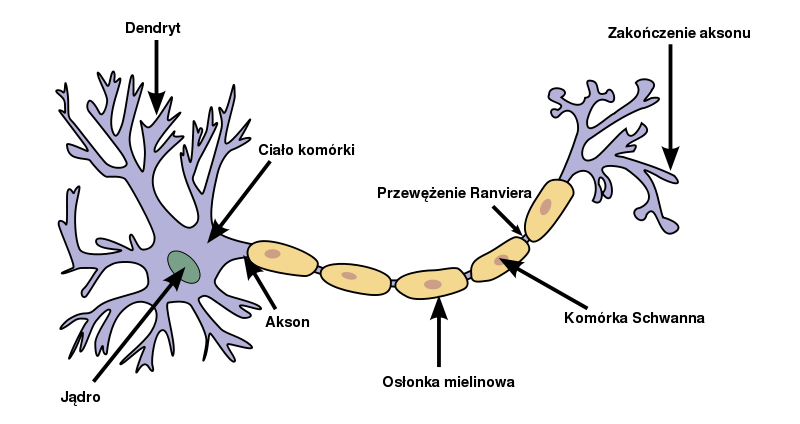
\includegraphics[scale=0.5]{images/neuron.png}
\caption{Model neuronu}
\end{figure}

\begin{enumerate}
\item Komórka nerwowa wyposażona jest jądro komorkowego, wiele końcówek komórki nazywane dendrytami oraz pojedynczą końcówekę nazywaną aksonem.
\item Neurony komunikują się ze sobą wysyłając do siebie elektrochemiczne (elektryczne w komórce, chemicznie na łączeniu) sygnały.
\item Neuron w trybie gotowości prowadzi nasłuchiwanie i czeka na pobudzenie elektryczne na dowolnym z jego dendrytów . 
\item Kiedy zostanień pobudzony poprzez dowolny z dendrytów, wyznaczana jest wartość wewnętrznego stanu neuronu.
\item Jeśli stan te przekracza pewien poziom progowy, neuron przechodzi w tryb aktywności i otrzymywaną energię zaczyna w postaci wzmocnnionej przekazywać.
\item Jeśli neuron przechodzi w stan aktywności, to za pomocą jego aksonu przekazywane jest do sąsiadów rozważanego neuronu - sygnał w stanie pobudzenia.
\item Połączenia prowadzące do aktywacji neuonów powodują wzmacnianie ich wpływu na końcowy egekt działania kodu.
\end{enumerate}

\begin{figure}
\centering 
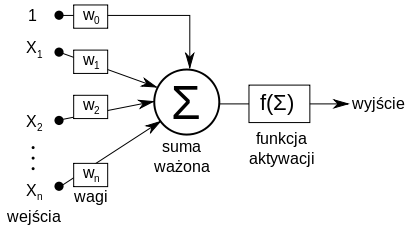
\includegraphics[scale=0.5]{images/model_neuronu.png}
\caption{Model neuronu McCullocha i Pittsa.} \label{fig.chapter.predictions.neuron.model}
\end{figure}

W roku 1943 opracowany został matematyczny model neuronu autorstwa  McCullocha i Pittsa opisane np. na grafice \ref{fig.chapter.predictions.neuron.model}. Wyszczególniam on pojęcia takie jak:
\begin{itemize}
\item Funkcja aktywacji - transformacja, której poddawany jest łączny sygnał z wejść, przed oceną przekroczenia progu aktywacji.  
\item Wagi - parametry opisujące początkową ocenę sygnału odczytanego przez dendryty.
\item Bias - opisujący przesunięcie poziomu aktywacji,
\item Wejścia/ wyjścia opisujące początek i koniec przetwarzania.
\item Wartwa ukryta czyli grupy neuronów nie stanowiących ani początkowego, ani końcowego etapu przekształcania. 
\end{itemize}

\subsubsection{Rodzaje sieci neuronowych}

Najbardziej podstawowy podział neuronów odbywa się z uwagi na funkcję aktywacji:
\begin{itemize}
\item Adaline - funkcja aktywacji jest identycznością
\item Perceptron - funkcja aktywacji jest signum lub podobną funkcją
\item Sigmoidalny - funkcja aktywacji jest funkcja podobna do signum, ale różniczkowalna
\begin{itemize}
\item unipolarna $ f(x) = \frac{1}{1+e^{-\beta x}}$
\item bipolarna $ f(x) = \frac{2}{1+e^{-\beta x}} -1$
\end{itemize}
\end{itemize}

Znacząca siła sieci neuronowych (ANN) płynie z łączenia neuronów w duże struktury.

Wyróżniamy:
\begin{itemize}
\item (FNN) Sieci gdzie neurony są połączone w warstwy i przetwarzane kolejno. Sieci w których nie ma cykli pomiędzy neuronami nazywamy sieciami jednokierunkowymi.
\item (RNN)Sieci gdzie występują cykle nazywamy rekurencyjnymi. Lub sieciami z pamięcią, gdyż wtedy w sieciach ukrywają się informacje z przekształceń dla poprzednich danych.
\item Dopasowane do zadań o szczególnej specyfikacji.
\item (CNN) Sieci splotowe.
\item Sieci głębokie.
\end{itemize}

\begin{remark*}
Dla większości sieci neuronowych nie zostały opracowane matematyczne dowody zbieżności procesu uczenia. Zbieżność danego rodzaju sieci do danego problemu są z reguły potwierdzane na kanwie eksperymentów numerycznych.Rozwiązania za pomocą sieci neuronowych są zatem heurystykami.
\end{remark*}

\subsection{Sieci jednokierunkowe}
W niniejszej części skupimy się na sieciach jednokierunkowych - sieciach najprostszych - i nie oszukując się - dogłębnie już przebadanych.
\begin{figure}
\centering
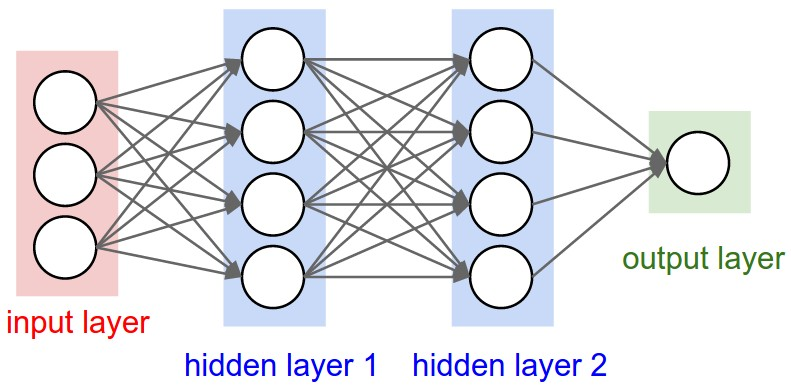
\includegraphics[scale=0.3]{images/siec_neuronowa.jpg}
\caption{Jednokierunkowa sieć neuronowa.} \label{fig.chapter.predictions.FNN.schemat}
\end{figure}

Nasze sieci neuronowe w większości przypadków działają w trybie uczenia nadzorowanego. Dysponujemy zatem zbiorem treningowym postaci $ Tren = \set{ (x,y), x \in \setR^n, y \in \setR^m}$, gdzie $x$ są wektorami cech objaśniających, a $y$ są wektorami cech objaśnianych. Przez $w$ oznaczmy wektor wektorów współczynników sieci (niekoniecznie macierz bo warstwy mogą być różnoliczne). Przez $F$ oznaczmy natomiast całe przekształcenie związane z siecią.

Chcąc wyjaśnić zależność pomiędzy cechami $X$ a cechami $Y$ przypuszczamy istnienie funkcji $G$ takiej, że 
\begin{equation*}
y = G(x),
\end{equation*}
spełnionej dla każdego $x$ i każdego $y$. Następnie przypuszczamy, że funkcję $G$ daje sie aproksymować za pomocą funkcji z klasy $x \mapsto F(w,x)$. 

Poszukujemy naszej odpowiedniej aproksymacji w następujący sposób:
\begin{enumerate}
\item Losujemy początkowy stan wektora wag.
\item Bierzemy element ze zbioru treningowego $(x,y) \in Tren$ i przekształcamy go przez naszą sieć.
\begin{equation*}
\hat{y} = F(w,x).
\end{equation*}
\item Wyznaczamy błąd naszego układu wag, z reguły zdefiniowany jako błąd średniokwadratowy na wyjściu
\begin{equation*}
Error = \sum_{i = 1}^{m} (y_i - \hat{y}_i)^2
\end{equation*}
\item Poprawiamy układ wag celem zmiejszenia błędu sieci.
\end{enumerate}

\subsubsection{Algorytm wstecznej propagacji błędu}

Wzór na błąd dla elementu zbioru treningowego $(x,y) \in Tren$ można zapisać jeszcze inaczej
\begin{equation*}
Error(w) = \sum_{i =1 }^{m} (y_i - F(w,x)_i)^2.
\end{equation*}
Zauważmy, że wszystkie wagi sieci mają aktywny udział w popełnianiu błędu. Widzimy również, że błąd popełniany przez kolejne neurony wpływa na błąd popełniany przez neurony kolejnych warstw. Jednak tylko dla wektorów ostatnich warstw możemy łatwo policzyć błąd
\begin{enumerate}
\item Błąd popełniony przez $i$-ty neuron ostatniej warstwy to $(y_i - \hat{y}_i)^2$,
\item Błąd popełniany przez $j$-tą wagę tego neuronu powinien być proporcjonalny do jej udziału w utworzeniu $\hat{y}_i$,
\item Błędy popełniane przez poprzedzające warstwy wyznaczane są jako sumy błędów popełnionych przez wagi dla danego wejścia w warstwie wyżej.
\item Błąd popełniony przez $i$-ty neuron ostatniej warstwy to $(y_i - \hat{y}_i)^2$,
\item Błąd popełniany przez $j$-tą wagę tego neuronu powinien być proporcjonalny do jej udziału w utworzeniu $\hat{y}_i$,
\item Błędy popełniane przez poprzedzające warstwy wyznaczane są jako sumy błędów popełnionych przez wagi dla danego wejścia w warstwie wyżej.
\end{enumerate}

Wprowadzanie poprawki w wektorach wag jest zadaniem z zakresu optymalizacji wielowymiarowej. Najczęściej do jej rozwiązywania stosujemy algorytm najszybszego spadku wprowadzający poprawki wg. zasady (oznaczmy $w^{i,j}_k(t)$ jako $k$-tą wagę w $j$-tym neuronie $i$-tej warstwy w $t$-tej iteracji)

\begin{equation*}
w^{i,j}_k(t+1) = w^{i,j}_k (t) - \eta \ddx{w^{i,j}_k(t)} Error(w)
\end{equation*}

Współczynnik $-\eta$ jest parametrem danego procesu uczenia, $\eta \in (0,1)$. Zapewnia wykonanie przesunięcie wektora wag danego neuronu w kierunki przeciwnym do gradientu funkcji w tym punkcie (czyli przesunięcie ku największemu spadkowi).  Wprowadźmy następujące oznaczenia:
\begin{description}
\item[$M$] - ilość warstw sieci
\item[$i$] - licznik warstw sieci
\item[$N_i$] - ilość neuronów w i-tej warstwie
\item[$j$] - licznik neuronów w danej warstwie
\item[$k$] - licznik wejścia w danym neuronie. Ograniczony przez ilość neuronów warstwy poprzedniej
\item[$x$] - wektor na wejściu sieci
\item[$y$] - wektor na wyjściu sieci
\item[$\hat{y}$] - odpowiedź sieci na wektor $x$
\item[$x_i$] - wektor na wejściu i-tej warstwy sieci $x_1 = x$
\item[$y_i$] - wektor na wyjściu i-tej warstwy sieci $y_i = x_{i+1}$ oraz $y_M = \hat{y}$.
\item[$f$] - funkcja aktywacji neuronu
\item[$F$] - funkcja odpowiadająca całości sieci
\item[$s^{i,j}$] - wartość iloczynu skalarnego wag $j$-tego neuronu $i$ tej warstwy przez wektor wejścia $i$-tej warstwy
\item[$w^{i,j}$] - wektor wag $j$-tego neuronu $i$ tej warstwy
\item[$w^{i,j}_k$] - $k$-ta waga $j$-tego neuronu $i$-tej warstwy
\item[$w^{i,j}_k(t)$] - $k$-ta waga $j$-tego neuronu $i$-tej warstwy w $t$-tej iteracji.
\end{description}

Wtedy 
\begin{equation*}
w^{i,j}_k (t+1) = w^{i,j}_k(t) - \eta \delta^{i,j} x^{i}_k
\end{equation*}
gdzie
\begin{eqnarray*}
\delta^{M,j} &= -( y_j - f(s^{M,j} ))  f'(s^{M,j}), \\
\delta^{i,j} &= f'(s^{i,j}) \sum_{l=1}^{N_{i+1}} \delta^{i+1,l} w^{i+1,l}_j.
\end{eqnarray*}

\subsubsection{Czemu sieci działają}

Aby zrozumieć motywację za działaniem sieci przypomnijmy sobie zasadę działania klasyfikatora liniowego (obrazek 
\begin{figure}
\centering
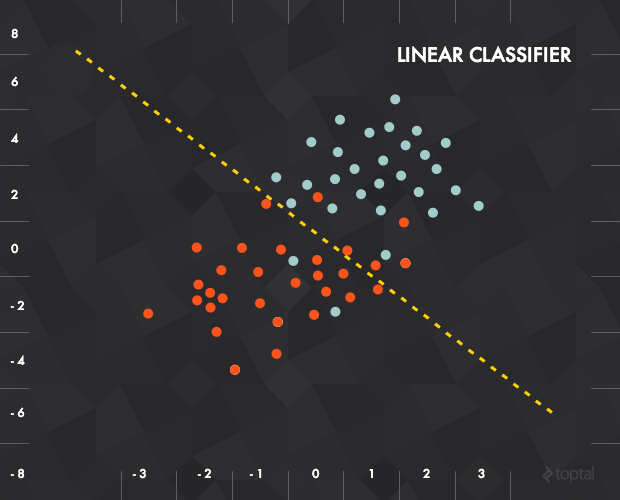
\includegraphics[scale=0.3]{images/klasyfikator_liniowy.png}
\caption{Schemat klasyfikatora liniowego}
\label{fig.chapter.predictions.linear.ann}
\end{figure}

Natomiast w przypadku gdy dane są nieseparowalne liniowo:
\begin{figure}
\centering
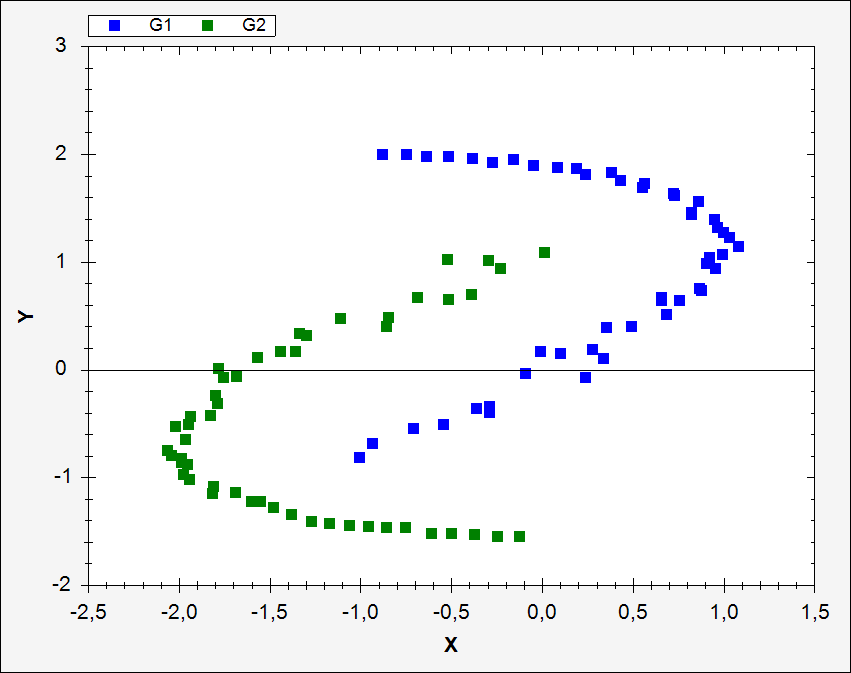
\includegraphics[scale=0.3]{images/nieseparowalne_dane.png}
\caption{Przykład danych nie separowalnych}
\label{fig.chapter.predictions.linear.ann.not.separable}
\end{figure}

Sieci neuronowe uzyskują wyraźną przewagę nad klasyfikatorem liniowym.
\begin{itemize}
\item Funkcje działającej w neuronach są ciągłe, różniczkowalne, odwracalne etc.
\item Sieć całościowo dokonuje dyfeomorficznego przekształcenia wielowymiarowej przestrzeni $\setR^n$
\item Prowadzi to transformacji danych do postaci liniowo separowalnej
\item Dzieje sie w przestrzeniach o takiej ilości wymiarów, że nie są w stanie pokazać tego żadnego wykresy
\end{itemize}

Nie każda sieć potrafi wytworzyć odpowiedni rodzaj dyfeomorfizmu. Najważniejszym uczestnikiem jest funkcja aktywacji oraz sposób w jaki $x$ jest wprowadzany do niej. Przyjrzyjmy się \ref{fig.chapter.predicition.separability.2} oraz temu jak po wzroście ilości wymiarów nasze zadanie staje wydatnie separowalne \ref{fig.chapter.predicition.separability.3}

\begin{figure}
\centering
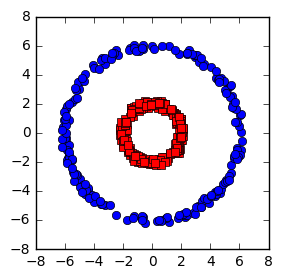
\includegraphics[scale=0.3]{images/nieseparowalne_dane2.png}
\caption{Przykład braku separowalności danych} \label{fig.chapter.predicition.separability.2}
\end{figure}

\begin{figure}
\centering
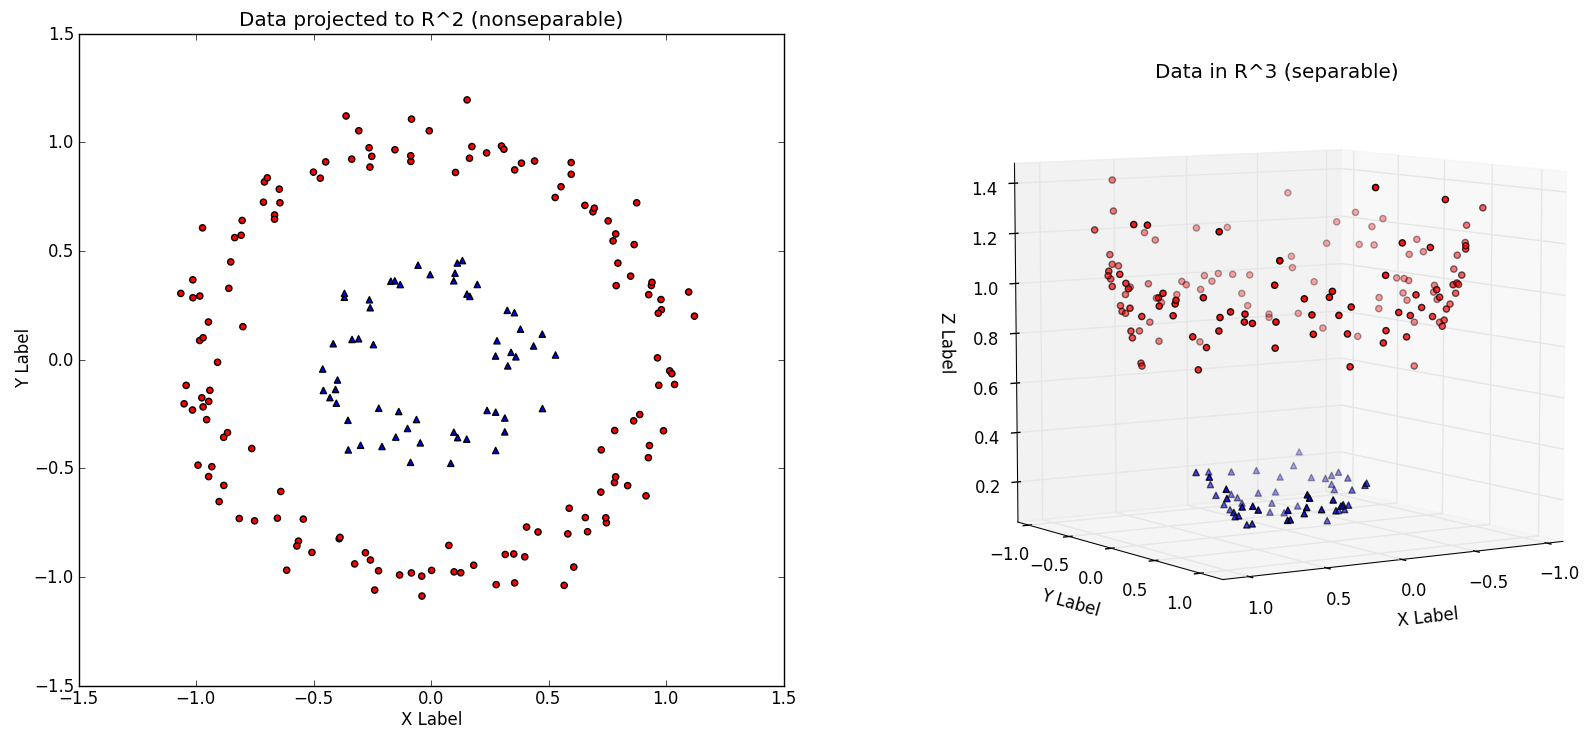
\includegraphics[scale=0.15]{images/jednak_separowalne.png}
\caption{Przykład jednak separowalnych danych} \label{fig.chapter.predicition.separability.3}
\end{figure}

\subsection{Sieci rekurencyjne}

Wszystkie sieci, które nie są jednokierunkowymi - są sieciami rekurencyjnymi. W sieciach tych występują tzw. sprzężenia zwrotne, a więc informacje wychodzące z pewnego neuronu mogą jeszcze do niego powrócić. Sieci takiej postaci okazują się dobrze modelować zjawiska z pamięcią - czyli np. szeregi czasowe, w których predykcja zależy silnie od wcześniejszych informacji o zjawisku. Innym obszarem zastosowań tego rodzaju sieci są problemy optymalizacyjne. Najpopularnieszym rodzajem sieci tego typu są Sieci Hopfielda

\subsubsection{Sieci Hopfielda}

%TODO uzupełnić

\subsection{Sieci splotowe}

%TODO uzupełnić

\subsection{Sieci głębokie}

Głebokie sieci neuronowe stanowią jeden z najbardziej (jeśli nie najbardziej) obiecujących postępów technologicznych naszych czasów. Sieci tego rodzaju pozwoliły na uzyskanie znakomitych komputerowych rozwiązań dla bardzo trudnych problemów komputerowych.

Rozważmy kilka problemów, z którymi można spotkać się w codziennym życiu, lub pracy zawodowej.

\begin{problem*}
Jednym z najprężniej rozwijanym działów komputerowych, i jednocześnie posiadającym bardzo znaczne fundusze, jest sektor gier komputerowych. Wiele z tych opiera się w swoim działaniu o rywalizację pomiędzy graczem, a komputerowo wygenerowanym przeciwnikiem. Jednym z podstawowych wskazań postępu rozwoju danej gry jest określenie stopnia inteligencji jaką wykazują się cyfrowi przeciwnicy. Biorąc pod uwagę, że człowiek jest istotą uczącą się - jednego można być pewnym. Wraz ze wzrostem umiejętności gry człowieka - jego oczekiwania w zakresie cyfrowych przeciwnków rosną jednakowo.
\end{problem*}

\begin{problem*}
Rozważmy inny problem. Gry są pewnego rodzajami symulacji, w których znajdujemy się w sytuacjach dla siebie nietypowych.
\begin{itemize}
\item Wojna, walka - choć gry tego dotyczące są bardzo popularne, niewiele z nas ma życzenie wziąć udział w prawdziwym konflikcie zbrojnym,
\item Zarządzanie dużym przedsiębiorstwem - tu często chętnie byśmy znaleźli w sytuacji pewnego bogatego człowieka, zmuszonego do zarządzania przedsiębiorstwem. Choć znaczna część nas by łatwo pogodziła sie z dodatkowymi pieniędzmi, już mniej chętnie podjęłaby się obowiązków pełnionych przez tego człowieka.
\item Wyścigi sporty -  podobnie pozwala nam to sprawdzać się w sytuacjach, które normalnie wymagałyby od nas tytanicznej pracy, i jeszcze zostawiały nas mocno zmęczonymi.
\end{itemize}
Wirtualne symulacje mogą jednak dotyczyć nie naszej rozrywki, ale naszego szkolenia. Wyobraźmy sobie, żołnierzy ćwiczących na symulatorach, manewry samolotem, czołgiem, łodzią podwodną lub bezpośrednią walką, strzelanie. Jeśli symulacje treningowe okażą się wysokiej jakości - być może ocalą później życie żołnierza w boju. Zapewnią mu rutynę, którą potrzebuje by uzyskać wysoki stopień skuteczności. Co ze szkoleniami dla policji, straży pożarnej?
\end{problem*}

\begin{problem*}
Kolejnym popularnym ostatnio problemem jest powracający temat pojazdów autonomicznych. Badania statystyków pokazały, że przeciętny amerykanin w czasie swoje życia spędza ponad 2 lata w samochodzie, przemieszczając się. Automatyczne sterowane pojazdy to nie tylko oszczędność czasu, bo człowiek ten zamiast prowadzić samochód mógłby realizować inne cele 
\begin{itemize}
\item wykonać pewne zadania w swojej pracy,
\item poczytać książkę,
\item monitorować swoje życie społeczne (?! na to akurat szkoda czasu),
\item porozmawiać z rodziną (prowadząc samochód mamy ograniczone pole do takich akcji).
\end{itemize}
To poza tym wzrost bezpieczeństwa podróży (zawodny człowiek, zastąpiony przez niezawodne maszyny), ale oszczędność paliwa 
\begin{itemize}
\item Samochód może ograniczyć prędkość wiedząc, że zbliża się do czerwonego światła (choćby ono samo się jeszcze nie zapaliło),
\item Samochód może zmienić trasę na podstawie danych o ruchu, czy deklarowanej trasy innych pojazdów.
\item Może roztropnieć zarządzać przyśpieszeniem redukując skoki mocy silnika.
\end{itemize}
Wszystkie te rzeczy są do osiągnięcia wraz z konstrukcją takiego pojazdu. Podstawowym celem poprzedzającym jego powstanie - jest powstanie algorytmów pozwalającym samochodowi widzieć. Widzenie to bowiem coś więcej niż patrzenie. Patrzeć potrafi kamera, czy oko. Jednak dopiero umysł człowieka jest w stanie uporządkować te informacje by dostrzec przeszkodę, możliwość czy zagrożenie. Algorytmy automatycznego rozpoznawania na obrazach są tu nieodzowne.  
\end{problem*}

\begin{problem*}
A może komputer który wspiera proces leczania, poprzez asystowanie lekarzowi w zakresie diagnostyki, lub wczesnego pogorszenia stanu zdrowia.
\end{problem*}

\begin{problem*}
A może komputer komponujący nową muzykę? Albo muzykę podobną do danej. Może program, który próbuje zinterpretować dany utwór tak jakby jego cover wykonywał zespół Queen, czy Elvis Presley lub Frank Sinatra.
\end{problem*}

\begin{problem*}
A może algorytm, który rozpoznaje trendy na rynkach finansowych? Algorytm, który znajduje tę jedną prostą sztuczkę przez którą maklerzy z całego świata zaczynają Ciebie nienawidzić. Kto by nie chciał czegoś takiego.
\end{problem*}

Na całym świecie poszukiwane są obecnie różne konfiguracje głębokich sieci neuronowych i rozpoznawane w zakresie ich zastosowania do rozwiązania między innymi problemów wylistowanych powyżej.

Rodzi się pytanie czego potrzeba aby stosować głębokie uczenie i głębokie sieci. Odnosząc sie do omówionych juz jednokierunokowych sieci neuronowych - w sieciach głębokich mamy doczynienia z 
\begin{enumerate}
\item Dużo większej liczby neuronów,
\item Dużo większej liczby warstw (miały być głębokie),
\item Bardziej skomplikowanych połączeń między warstwami (nie wszystko ze wszystkim bez przekształceń),
\item Większa moc obliczeniowa,
\item Zaufanie strukturom sieci na wyznaczenie istotnych cech.
\end{enumerate}

Do przeprowadzania analizy tymi metodami niezbędne jest zatem kilka elementów:
\begin{itemize}
\item Posiadanie komputera (lub odpowiedniego dostępu) do komputera o znacznej mocy obliczeniowej,
\item Przydatna jest wiedza z zakresu algebry liniowej i przekształceń wektorów macierzy - w żaden bowiem sposób nie umiemy uciec od zagadnień wstępnego preprocessingu danych,
\item Podstawowa wiedza z zakresu rachunku prawdopodobieństwa - gdyż proces uczenia jest w taki właśnie sposób rozumiany,
\item Solidna wiedza z zakresu technik uczenia maszyn. Poprzez ten punkt przydatna jest również wiedza z zakresu matematycznej optymalizacji wielowymiarowej.
\item Przydaje się wiedza z programowania w Pythonie, biorąc pod uwagę, że Tensorflow jest głównym narzędziem uczenia głębokiego.
\end{itemize}

W niniejszej pozycji nie będziemy skupiać się na rozpisaniu całego uczenia głębokiego - postaramy się skupić na wyjaśnieniu ogólnego konceptu ich użycia, oraz omówić istniejące zastosowania ich w tematyce analizy danych wielowymiarowych - w tym i analizy np. obrazów - które są szczególną postacią danych wielowymiarowych.

\chapter{Modele decyzyjne Markowa}

\section{Podejmowanie decyzji w warunkach niepewności}

W dalszej części niniejszego skrytpu zastanawiamy się nad szerszą perspektywą związaną z predykcją. Wszystko to zaczyna się od istotnego pytania:

\textit{Do czego potrzebujemy predykcji?.}

Predykcja przecież czemuś musi służyć, jakiemuś szerszemu celowi.
Co możę być celem predykcji?

\begin{itemize}
\item W przypadku prognozy pogody może to podpowiedzieć czy należy wziąć parason, rozpocząć żniwa, czy też zakupić wycieczkę nad polskie morze,
\item W przypadku wartości giełdowej, pozwoli nam to na odpowiedzenie na pytanie czy kupić jakiś produkt, sprzedać lub przechować,
\item W przypadku dobowej sprzedaży w jakimś sklepie, pozwoli nam to okreslić ilości wymaganych zapasów i w efekcie zminimalizować koszty składowania i psucia się produktów. 
\end{itemize}

Podsumowująć powyższą listę można dojść do prostego wniosku. Dzięki predykcji, podstawową umiejętność którą zdobywamy jest możliwość podejmowania decyzji dotyczących przyszłości. Biorąc pod uwagę to, że predykcja jest obarczona modelami probabilistycznymi należy nazwać to podejmowaniem decyzji w warunkach niepewności. Powiedzmy sobie zatem co nie co o modelach podejmowania decyzji.

\subsection{Najprostszy modele podejmowania decyzji}

W najprostszym modelu podejmowania decyzji można wyszczególnić jedynie kilka elementów:
\begin{itemize}
\item Pojedynczy model predykcyjny, generujący predykcję przyszłej wartości zjawiska, oraz
\item Funkcje przypisującą do konkretnych przedziałów wartości możliwe decyzje. Funkcje takie najczęściej mają konstrukcje progową. Jeśli przekroczona jest wartość prognowa należy wykonać pewną akcję. Jeśli przeciwnie, wykonać drugą akcję. 
\end{itemize}

Istotnie nie ma tu wielkiego poziomu skomplikowania. I mogłoby się wydawać, że prostota ta zapewnia nam wszystko co jest na potrzebne. Zapewne tak by właśnie było w idealnym wszechświecie, gdzie odnajdujemy jeden najwłaściwszy model predykcyjny, gdzie estymujemy właściwe statystyki, a dane testowe są doskonale reprezentatywne dla zjawiska. Jak łatwo się domyslić - w praktyce - nie mamy możliwości pracowania z tak dobrymi modelami predykcyjnymi, by ten najprostszy model podejmowania decyzji okazał się trafionym.

Trzeba rozpocząć ogólniejsze rozważania.

\subsection{Nie tak już proste modele podejmowania decyzji} 

Aby dostrzeć inne rodzaje sposobu podejmowania decyzji trzeba się zastanowić. By dostrzec model, trzeba zauważyć jego wdrożenia i stworzyć uogólnienie. To z kolei rodzi pytanie:

\textit{Czy my już kiedyś podejmowaliśmy decyzje w warunkach niepewności?.}

Jesteśmy w stanie wymienić przynajmniej jeden przypadek. W ramach tego skryptu już wielokrotnie podejmowaliśmy decyzję dotyczącą wyboru danego modelu predykcyjnego. Teraz drugie pytanie:

\textit{Na jakiej podstawie podjęliśmy decyzje co do wyboru modelu?}

Na różnych etapach były to różne przesłanki. Można je zgrupować w następujące podgrupy:

\begin{itemize}
\item Wybieraliśmy funkcję błędu i znajdowaliśmy dla nich optymalne parametry modelu (minimalizacja funkcjonału błędu). Potencjalnie rozważać możemy różne jej postacie.
\item Ocenialiśmy jakość modeli na podstawie np. wykresów diagnostycznych, czy cech statystycznych ($R^2$),
\item Rozważaliśmy różne stopnie modeli i stosowaliśmy funkcjonały błędu z poprawkami na kształt modelu (AIC, AICC, BIS),
\item W reszcie testowaliśmy efekty predykcji na zbiorze testowym, chcąc porównać różne modele o zupełnie różnych konstrukcjach.
\end{itemize}

Jakie stąd można wysnuć wnioski? Do podjęcia decyzji wykorzystaliśmy wiele informacji, o różnym charakterze, wyliczonych na podstawie różnych formuł. Podobny algorytm możemy zastosować w kontekście podejmowania decyzji na podstawie naszych modeli predykcyjnych. 

\begin{problem*}
Rozważmy przypadek w którym mamy zespół, który ma wesprzeć podjęcie decyzji biznesowej w firmie. Zespoł dzieli się i wytwarza kilka modeli - które ocenia jako obiecujące. Wsród nich można oczywiścia wskazać model najlepszy. Jaką podjąć decyzje na podstawie tych informacji.
\end{problem*}

Jeszcze chwilę temu podjęlibyśmy decyzję wskazaną przez najlepszy model, sposród tych wytworzonych przez różne podzespoły. Obecnie jednak dostrzegamy już w tym, że wszelkie informacje ozyskane przez nieco gorsze modele byłyby odrzucone. Zatem obecnie już decyzję podjęlibyśmy patrząc na informacje zwrócone przez wszystkie modele predykcyjne i na tej podstawie podjęlibyśmy łączną decyzję.

\begin{problem*}
Przyjmijmy, że mamy 7 modeli predykcyjnych. Na tej podstawie musimy podjąć decyzję biznesową. Model wykazujący się w testach najniższym błędem każde podjać decyzję A. Pozostałe 6 modeli wskazuje że należy podjąć decyzję B. Czy podjęcie ostatecznie decyzji B jest bezzasadne?
\end{problem*}

\begin{definition}[Prosty model podejmowania decyzji]
Rozważmy model podejmowania decyzji składający się z 
\begin{itemize}
\item Rodziny modeli predykujących jedną zmienną,
\item Rodziny funkcji przypisujących akcję do wartosci zmiennej z danego modelu predykującego, oraz
\item Funkcji tworzącej łączną decyzję na podstawie decyzji płynących z pojedynczych modeli (syntezator).
\end{itemize}
\end{definition}

W dalszej części omówimy zupełnią inną metodą podchodzenia do tematu modeli decyzyjnych, opartą o teorię Łańcuchów Markowa.

\section{Preliminaria do modeli decyzycjnych Markowa}

\subsection{Łańcuchy Markowa, Własność Markowa}

Zanim przejdziemy do samych procesów decyzyjnych przypomnijmy czym są Procesy Markova lub inaczej nazywane Łańcuchy Markowa. 

Rozpatrzmy ciąg zmiennych losowych $\sequence{X_n}{n\in \setN }{}$ określonych na tej samej przestrzeni probabilistycznej $(\Omega, \sigmaalgebra{F},P)$. Zmienne te niech mogą przyjmować jedynie skończoną liczbę wartości (nazywane stanami).

\begin{definition}[Własność Markowa]
Powiemy, że ciąg zmiennych losowych (takich jak wyżej) ma własność Markowa (jest łańcuchem Markowa) gdy dla każdego $n \in \setN$ oraz każdego ciągu stanów $s_0, s_1, \ldots, s_n \in S$ mamy
$$
P(X_n = s_n | X_{n-1} = s_{n-1}, X_{n-2} = s_{n-2}, \ldots, X_1 = s_1) = 
P(X_n = s_n | X_{n-1} = s_{n-1}),
$$ 
czyli gdy prawdopodobieństwa znalezienia sie w danym stanie zależą jedynie od stanu go poprzedzającego.
\end{definition}

\begin{definition}[Macierz stochastyczna]
Macierz gromadząca prawdopodobieństwa przejścia z i-tego stanu do j-tego stanu taka, że sumy poszczególnych wierszy wynoszą $1$ to macierz taką nazywamy macierzą przejścia lub macierzą stochastyczną.
\end{definition}

\subsection{Skończone gry z światem i agentem.}

Modele decyzyjne poruszają się w tzw. skończonych światach. Ponadto wyszczególnia się w nich dwie role świat oraz agentów (czasami konkurujących ze sobą). 
\begin{itemize}
\item Świat reprezentuje ogół stanów w jakich znajdują się wszystkie z nim znajdujące sie twory. Często nie cała informacja o świecie jest dostępna agentom.
\item Agenci są inteligentnymi i zdolnymi do podejmowania decyzji konstruktami osadzonymi w danym świecie. 
\end{itemize}  

\begin{problem*}
Rozważmy następujące zagadnienie. Mamy dostępny następujący świat jak na grafice \ref{fig-grid-deterministic}. Załóżmy, że mamy dostępne następujące składowe tego modelu:
\begin{itemize}
\item 4 akcje, które można wykonać to ruch w górę-dół-lewo-prawo.
\item Efekty akcji, powodujące ruch o ile tylko pole w danym kierunku jest dostępne oraz pozostanie w tym samym polu jeśli pole nie jest dostępne. \ldots
\item 2 stany pochłaniające \ldots
\item Pytanie o akcje które należy wykonać aby przejść ze startu do skarbu w najkrótszy sposób?
\end{itemize}
\end{problem*}

\begin{figure}
\centering
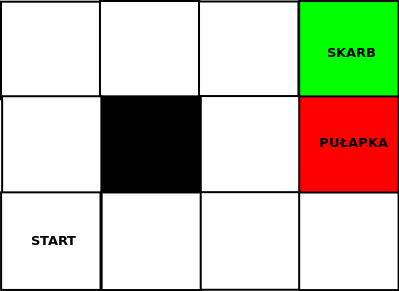
\includegraphics[scale=0.3]{grids/deterministyczny.png}
\caption{Skończony świat deterministyczny} \label{fig-grid-deterministic}
\end{figure}

Mamy dostępne dwa rozwiązania optymalne \ref{fig-grid-deterministic-1sol} oraz \ref{fig-grid-deterministic-2sol}.

\begin{figure}
\centering
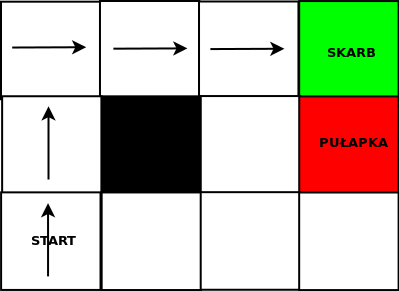
\includegraphics[scale=0.3]{grids/det_solution1.png}
\caption{Rozwiązanie optymalne 1} \label{fig-grid-deterministic-1sol}
\end{figure}

\begin{figure}
\centering
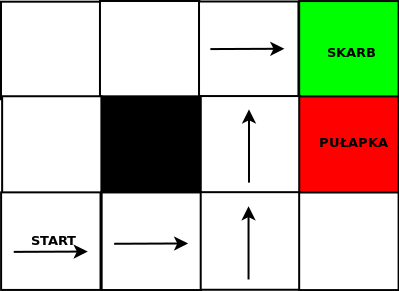
\includegraphics[scale=0.3]{grids/det_solution2.png}
\caption{Rozwiązanie optymalne 2} \label{fig-grid-deterministic-2sol}
\end{figure}

\section{Modele decyzyjne Markova}

Jak mawia klasyk:

\begin{quotation}
Chcieliśmy dobrze, wyszło jak zawsze. (zwykle)\\
\begin{flushright}
Wiktor Czernomyrdin, polityk rosyjski (1938-2010).
\end{flushright}
\end{quotation}

Prowadzi to do pewnej refleksji, którą mamy po przemyśleniu skończonych światów deterministycznych. Obserwujemy, że akcje które podejmujemy:
\begin{itemize}
\item Mogą powodować zamierzony efekt, przeciwny efekt, inny efekt, niezamierzony efekt lub nawet brak efektu.
\item Efekty akcji należy rozumieć w kanwie rachunku prawdopodobieństwa.
\item Rozważać dalej będziemy świat, rządzone przez prawdopodobieństwa - tzw. {Światy (modele) stochastyczne}.
\end{itemize}

\begin{problem*}
Rozważmy poprzednio omówiony świat (rysunek \ref{fig-grid-deterministic}) z następującym zestawem zasad:

\begin{itemize}
\item Bez zmian - 4 akcje, efekty akcji, 2 stany pochłaniające \ldots
\item Wybrana akcja $a$ wykonuje się poprawnie z pr-stwem $0.8$,
\item Z pr-stwem $0.1$ wykonuje się ona prostopadle w lewo względem zamierzonej tj. zamiast w dół to w prawo.
\item Z pr-stwem $0.1$ (brakujące prawdopodobieństwo) wykonana zostanie akcja prostopadle w prawo względem zamierzonej tj. zamiast w lewo to w górę.
\end{itemize}
\end{problem*}

\begin{exercise*}
Rodzi się następujące pytanie. Jakie jest prawdopodobieństwo, że realizując kolejno nasze akcje z wersji świata deterministycznego dotrzemy do skarbu?
\end{exercise*}

\begin{proof}[Rozwiązanie]
Występują dwie niezależne drogi, w których nasza strategia zadziała. Pierwsza gdy wszystkie nasze akcje wykonają się poprawnie
$$
0.8 \cdot 0.8 \cdot 0.8 \cdot 0.8 \cdot 0.8 = 0.8 ^5 = 0.32768.
$$
Oraz druga gdy pomimo błędów dotrzemy do rozwiązania
$$
0.1 \cdot 0.1 \cdot 0.1 \cdot 0.1 \cdot 0.8 = 0.8 \cdot 0.1^4 = 0.00008. 
$$

Zatem ostatecznie nasze prawdopodobieństwo to: $0.32768 + 0.0008 = 0.32776$. 
\end{proof}


\begin{definition}[Proces decyzyjny Markowa]
Procesem decyzyjnym Markova nazywać będziemy model składający się z 
\begin{itemize}
\item Stanów (skończona ilość) - pełne opisy położenia obiektu w świecie. ($s \in S$),
\item  Akcje (zbiór akcji) - wybory które można podjąć. Tu wystepować mogę dwie odmiany.
\begin{itemize}
\item Globalny zbiór akcji $A$,
\item lub lokalny zbiór akcji dostępnych w danym stanie $A(s)$.
\end{itemize}
\item Funkcji przejścia $T \colon S \times A \times S \to [0,1]$ zgodna z formułą:
$$
T(s, a, s') = P( s' | s, a ).
$$
Czyli oddający prawdopodobieństwa przejścia ze stanu $s$ do stanu $s'$ w efekcie wykonania akcji $a$. Funkcja ta stanowi opis świata, zbió© wszystkich praw jego fizyki,
\item  Nagrody , które mogą być wprowadzano na jeden z 3 sposobów:
\begin{itemize}
\item Nagroda za przebywanie w danym stanie $R(s)$,
\item Nagroda za przebywanie w danym stanie i podjęcia danej decyzji $R(s,a)$, oraz
\item Nagroda za przejście ze stany $s$ do stanu $s'$ w skutek decyzji $a$.
\end{itemize}
\end{itemize}
Do ważnych cech procesów decyzyjnych Markowa zaliczamy:
\begin{itemize}
\item Własność Markova (niezależność od stanów poprzedzających). Co inaczej oznacza, że liczy się tylko teraźniejszość. Tylko bieżący stan ma wpływ na określanie prawdopodobieństw. Oraz
\item Stacjonarność (niezależność od czasu). Łatwo tłumaczona na warunek określający, że \textit{Prawa fizyki się nie zmieniają} - albo po prostu, że zasady są stałe.\footnote{Dlatego funkcja przejścia nie posiada }
\end{itemize}
\end{definition}

Jeśli powyższe zatem definiuje nam problem to wyjaśnijmy również czym jest rozwiązanie takiego problemu:

\begin{definition}[Polityka]
Polityką nazwiemy dowolną funkcję $\pi: S \to A$, czyli przypisującą akcję do stanów. Przez naszę funkcję rozumiemy zatem relację grupującą trójki 
$$
\pi = \{ <s,a,r>, \ldots \}.
$$
\end{definition}

\begin{definition}[Rozwiazanie problemu decyzyjne Markowa]
Rozwiązaniem problemu decyzyjne Markowa nazwiemy tę funkcję $\pi^\ast: S \to A$, nazywaną polityką optymalną, która spośród zbioru wszystkich polityk danego problemu maksymalizuje wartość oczekiwaną nagrody.
\end{definition}

Ważnym jest zroumienie pewnej szczególnej różnicy

\begin{remark*}
Polityka to nie ciąg akcji zapewniajacy zysk (nie ciąg komend) - ale wskazówka (nakaz) co zrobić gdy znajdziemy się w określonym stanie (nawet gdy znaleźliśmy się w nim przez przypadek).
\end{remark*}

Niewątpliwie najtrudniejszą częścią całej tej teorii jest odszukanie polityki optymalnej. Nie jest to tak łatwe jakby się wydawało  W przypadku procesu decyzyjnego Markowa nagroda za dobre decyzje często może przyjść z bardzo dużym opóźnieniem. Rozważmy kilka przykładów

\begin{example}[Przykłady]

Rozważmy kilka obrazujących przykładów:
\begin{itemize}
\item Co zrobić mając do wyboru pójście na przyjęcie do znajomych względem uczenia się do egzaminu? Przyjęcie ze znajomymi może okazać się bardzo udane i wartość natychmiastowej nagrody może być wysoka - natomiast teoria z tego egzaminu - może się ostatecznie okazać nigdy nie zastosowana w późniejszym życiu. Z drugiej strony może okazać się, że nauka do egzaminu pozwoli nam w dalszej perspektywie uzyskać znacząco lepszą pracę i osiągnąć sukcesy w przyszłości.
\item Jaki ruch na szachownicy wykonać? W końcu być może 3 ruch spowodować, że 40 ruchów później partia będzie przegrana lub wygrana.
\item Jaki komputer, samochód, telefon, ubezpieczenie wybrać? W końcu tyle zmiennych może warunkować co się stanie w przyszłości.
\end{itemize}

\end{example}


Rozważmy kolejną wariację naszego problemu. Do tej pory większość stanu nie niosła ze sobą żadnej nagrody. Co się stanie kiedy to zmienimy?

\begin{problem*}
Wykorzystajmy ponownie naszą grafikę \ref{fig-grid-deterministic} z obrazem świata i zmodyfikujmy odpowiednio zasady tego świata.
Niech nasz świat to będzie opis pewnej plaży. Skarb to będzie chłodne w cieniu wraz ze stanowiskiem z lodami. Pułapką niech będzie część plaży cała w odłamkach szkła. Resztę niech pokrywa lekko gorący piasek. Obserwujemy następujące rzeczy

\begin{itemize}
\item Kiedy piasek nie parzył można było w nieskończoność poruszać się po stanach świata nie odczuwając presji na przemieszczanie się w kierunku nagrody. Osiągnięcia pola nagrody w 5 turze co i 105 zwracało efekt identyczny z punktu widzenia agentów tego świata.
\item Piasek lekko parzący powinien spowodować wymuszenie (względnie) szybkie przemieszczanie w kierunku pola z nagrodą. Symuluje to bowiem karanie agenta, za bezproduktywne trwanie w danym stanie.
\item Im bardziej parzący będzie piasek tym intuicyjnie agent będzie bardziej skłonny do podejmowania ryzyka celem unikania dużych kar.
\item Tak jak można dostrzec to w przypadku gdyby kary były faktycznie nagrodami - polityka sprowadza się do nie-kończenia-gry \ref{fig-paradise-sand}
\item Gdy stosowane są srogie kary (co powoduje zmianę plaży w świat parzącej lawy) \ref{fig-lava} - polityka optymalna nakazuje akcje szybko kończące grę.
\item Natomiast gdy kary są nieznaczne, jak na grafice \ref{fig-warm-sand}, obserwujemy to co wg nas jest najbardziej intuicyjną polityką.
\end{itemize}
\end{problem*}

\begin{example}[Pogląd Keynesa na inflację]
Osobą znające się dobrze matematyce finansowej są świadome dwóch poglądów na temat zjawiska inflancji. Jak wiadomo inflacja jest zjawiskiem, które powoduje osłabianie mocy nabywczej pieniądza w czasie. W efekcie tego wielu ekonomistów wskazuje, że zjawisko to należy zredukować do zera i pozwolić na swobodne i stacjonarne postrzeganie pieniądza. Jednak inna grupa ekonomistów stwierdziła, że efekty działania inflancji na rynek są inne. Grupa ta od twórcy podstaw tych koncepcji nazywa Keynesistami. Wg tej szkoły ekonomicznej
\begin{itemize}
\item Duża inflacja rujnuje ekonomię (oczywisty fakt),
\item Deflacja (ujemna inflacja - czyli pieniądz z czasem zyskuje na wartości) powoduje gromadzenie pieniądza i zahamowanie procesu handlu,
\item Brak inflacji tylko pozornie nie powoduje strat. W efekcie braku inflacji, tempo obrotu pieniądza jest wyraźnie zredukowane (ludziom nie śpieszy się wydawać pieniędzy).
\item Nieznaczna dodatnia inflacja powoduje pobudzenie wymiany handlowej, skłania do inwestowania pieniędzy zamiast ich prostego gromadzenia i powoduje rozwój gospodarczy.
\end{itemize}
\end{example}

Powyższy przykład jest podany celem umotywowania siły stosowania niewielkich kar do wymuszenia decyzji, które kierunkowane są na konkretny cel.

\begin{figure}
\centering
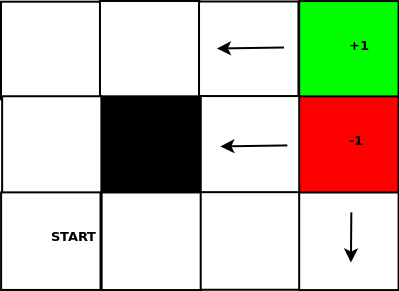
\includegraphics[scale=0.3]{grids/warm_world.png}
\caption{Optymalna polityka w świecie rajskiej plaży z $R(s) = +1$} \label{fig-paradise-sand}
\end{figure}

\begin{figure}
\centering
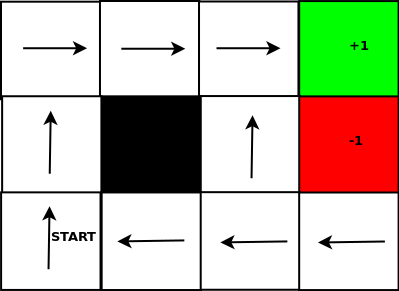
\includegraphics[scale=0.3]{grids/sand_solution.png}
\caption{Optymalna polityka w świecie plaży z $R(s) = -0.05$} \label{fig-warm-sand}
\end{figure}

\begin{figure}
\centering
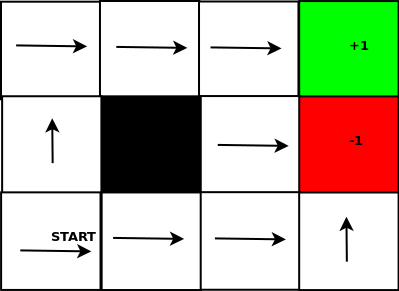
\includegraphics[scale=0.3]{grids/lava_world.png}
\caption{Optymalna polityka w świecie lawy z $R(s) = -1$} \label{fig-lava}
\end{figure}

\section{Koncepcja użyteczności w procesach decyzyjnych}

Ważnym elementem, który należy pamiętać - pracując z procesami decyzyjnymi - jest pamiętanie, że polityka nie określa nagrody za jej stosowanie.  To jest jedynie proste określenie wyboru akcji w danym stanie. Mając określoną politykę można określić wartość osiąganą przez pewne postępowania - ale w koncepcji procesów decyzyjnych - jest to sprawa drugoplanowa. Ponadto na tą chwilę miejmy również świadomość o występowaniu dwóch rodzajów procesów decyzyjnych w zależności o wiedzy o jego stanie.

\begin{definition}[Światy z informacją zupełną i niezupełną]
Powiemy, że dany świat jest światem z informacją zupełną jeśli dowolny agent - może poznać w pełni swój stan (w zależności od definicji - może to być również stan wszystkich agentów świata). Jeśli stan nie jest stanem z informacją zupełną to jest światem z informacją niezupełną. 
\end{definition}

Wreszcie przechodząc do oceny jakości stosowania danych polityk należy rozważyć dodatkowe pojęcia. Jak np. ciągi nagród.

\begin{definition}[Ciągi nagród, stanów, akcji]
W efekcie notowania postępów działania agentów tworzone są ciągi.
I tak
\begin{itemize}
\item Ciąg złożony ze stanów przez które kolejno przechodził wybrany agent - nazywa się ciągami stanów,
\item Ciąg złożony z wartości reprezentujących nagrody uzyskiwane przez wybranego agenta nazywa się ciągami nagród,
\item Ciąg złożony z akcji wybieranych przez agenta nazywa sie ciągami akcji.
\end{itemize}
Ponadto oznaczmy przez $SS$ przestrzeń wszystkich ciągów stanów, $SR$ przestrzeń wszystkich ciągów nagród oraz $SA$ przestrzeń wszystkich ciagów akcji.
\end{definition}

Zauważmy, że przez stacjonarność w problemach nasze ciągi nagród są potencjalnie nieskończone. Intuicyjnie ciągi nagród stanowia dla nas podstawę do oceny jakości danej polityki. Podstawa część naszego rozumowania na chwilę obecną może być opisana algorytmem:

\begin{enumerate}
\item Określamy pewną politykę, 
\item Ustalamy stan początkowy,
\item Stosując daną politykę możemy tworzyć ciagi nagród.
\end{enumerate}


\begin{remark*}
Ciągi nagród są zatem pewną realizacją szeregu czasowego.
\end{remark*}

Intuicyjnie czujemy, że aby uznać daną politykę za optymalną należy rozważać ciągi nagród generowane przez nią i je oceniać. Ciągi te są jednak potencjalnie nieskończone i wszystko to rodzi pytanie jak je oceniać. Do oceny stosowane są tzw. funkcje użyteczności.

\begin{definition}[Funkcja użyteczności]
Funkcja użyteczności nazywamy funkcję $U: SS \to \setR$. 
\end{definition}

Dzięki użyciu funkcji użyteczności możemy porównywać ciągi.

\begin{definition}[Porządek częściowy w przestrzeni $SS$ względem funkcji użyteczności $U$]
Powiemy, że dwa ciągi stanów $ ss^1 = (ss^1_0, ss^1_1, \ldots)$ oraz $ss^2 = (ss^2_0, ss^2_1, \ldots)$ spełniają relację częściowego porządku względem pewnej funkcji użyteczności $U$ gdy
$$
ss^1 \preceq ss^2 \iff U((ss^1_0, ss^1_1, \ldots)) \geq U((ss^2_0, ss^2_1, \ldots)).
$$

Ponadto jeśli $ss^1 \preceq ss^2$ oraz $ss^1 \succeq ss^2$ to napiszemy $ ss^1 \simeq ss^2$.
\end{definition}

\begin{problem}[Proste sumowanie nagród - przykład odrzucający model.]
Rozważmy przypadek gdzie funkcja użyteczności jest zadana jako prosta suma nagród w czasie, tj.
$$
U : (s_0, s_1, s_2, \ldots) : \mapsto \sum_{n=0}^{\infty} R(s_n).
$$
Rozważmy dwa ciągi nagród (dla odpowiednio ciagów stanów $s^1$ oraz $s^2$) postaci
$$
R(s^1) = (1,1,1,1,1,1,1,1,1,\ldots), \quad R(s^2) = (1,2,1,2,1,2,1,2,1,2,\ldots).
$$

Pomimo, iż intuicyjnie stwierdzilibyśmy, ze ciag stanów $s^2$ generuje lepsze ciągi nagród to widzimy, że
$$
U(s^1) = \infty = U(s^2),
$$
czyli w sensie tej funkcji użyteczności $s^1 \simeq s^2$ - czyli kompletnie nie to co sugeruje nam intuicja.
\end{problem}

Powyższy przykład powoduje rozbieżności z spodziewanym przez nas rezultatem gdyż rozważona funkcja użyteczności nie jest zgodna z naszym rozumowaniem. Stąd do rozwiazywania procesów decyzyjnych Markova używana jest przez nas inna klasa funkcji użyteczności.

\begin{definition}[Użyteczność Lambda]
Niech $\lambda \in (0,1)$. Funkcją użyteczność $U_\lambda : SS \to \setR$ nazywamy funkcję zadaną wzorem
$$
U: (s_0, s_1, \ldots) \mapsto \sum_{n=0}^{\infty} \lambda^n R(s_n).
$$
\end{definition} 

\begin{lemma}[Zbieżność w funkcji użyteczności lambda]
Niech $\lambda \in (0,1)$ oraz niech $R : S \to \setR$ nie przyjmuje wartości $\pm \infty$. Wtedy funkcja użyteczności lambda przyjmuje skończoną wartość dla wszystkich ciągów stanów.
\end{lemma}

\begin{proof}
Niech spełnione będą założenia z lematu. Niech $s = (s_0, s_1, \ldots)$ będzie pewnym dowolnym ciągiem stanów z przestrzeni $SS$. Wtedy
\begin{align*}
U(s) & = \sum_{n=0}^{\infty} \lambda^n R(s_n) \\
& \leq \sum_{n=0}^{\infty} \lambda^n \max \set{R_{max}, -R_{min}} \\
& = \max \set{R_{max}, -R_{min}} \frac{1}{1-\lambda} < \infty.
\end{align*}
Korzystamy w powyższym z tego, że przestrzeń stanów jest skończona - a zatem możliwe nagrody stanowią również skończony zbiór - więc można wskazać elementy maksymalne i minimalne. Reszta to własności ciągów geometrycznych.
\end{proof}

\begin{remark*}
Często faktyczną lambda użyteczność nagrody ze stanu $s_k$ tj $\lambda^i R(s_k)$ często jest nazywana zdyskonowaną nagrodą (i-krotnie zdyskontowaną). Przez to dostrzegamy kolejne analogie do matematyki finansowej czy ubezpieczeniowej.
\end{remark*}


\section{Równanie Bellmanna}

Powyżej zdefiniowane pojęcia pozwalają nam uporządkować algorytm oceny polityki. Mamy zatem:

\begin{enumerate}
\item Wybieramy konkretną politykę,
\item Ustalamy stan początkowy,
\item Generujemy postępując zgodnie z polityką ciągi stanów i nagród wychodzące z wybranego stanu początkowego,
\item Oceniamy je z użyciem funkcji użyteczności.
\end{enumerate}

Powyższe jednak nie uwzględnia stochastyczności modelu - przecież generowane ciągi stanów są losowe. Rozwiążmy ten problem dodając kolejny krok do algorytmu:

\begin{enumerate}
\item Wybieramy konkretną politykę,
\item Ustalamy stan początkowy,
\item Generujemy postępując zgodnie z polityką ciągi stanów i nagród wychodzące z wybranego stanu początkowego,
\item Oceniamy je z użyciem funkcji użyteczności.
\item Jako ocenę danej polityki przy starcie z danego stanu wybieramy wartość przeciętną uzyskiwanej użyteczności.
\end{enumerate}
Dokonując podsumowania po wszystkich stanach początkowych otrzymujemy postać wartość całej polityki. Pozwala to sformułować stwierdzenie.

\begin{theorem}[Postać polityki optymalnej]
Przy zastosowaniu funkcji użyteczności lambda z ustalonym $\lambda \in (0,1)$ polityka optymalna może zostać opisana wzorem
$$
\pi^\ast : s \mapsto \argmax_{\pi} \ExConditional{\sum_{t=0}^{\infty} \lambda^t R(s_n) }{ \pi, s_0 = s},
$$
gdzie przez $\ExConditional{\cdot}{\pi, s_0 = s}$ rozumiemy warunkową wartość oczekiwaną przy starcie z stanu $s$ oraz przestrzeganiu polityki $\pi$.
\end{theorem}

Powyższe twierdzenie dostarcza nam warunki dla polityki optymalnej, ale powyższa formuła nie wzbudza najmniejszych nadziei na obliczenie postaci dla rozważanego problemu. Aby pokazać jak można wykorzystać to do obliczenia realnej polityki danego problemu wprowadźmy dalsze oznaczenia.

\begin{definition}[Użyteczność stanu i polityki]
Niech $\pi$ będzie pewną polityką w naszym problemie decyzyjnym a $s$ pewnym stanem początkowym. Wtedy użytecznością nazwiemy funkcję 
$$
U : (\pi, s) \mapsto \ExConditional{\sum_{t=0}^{\infty} \lambda^t R(s_t) }{ \pi, s_0 = s}.
$$
Czasem z uwagi na stałość wyboru polityki będziemy pisać zamiast
$$
U^\pi(s) = U(\pi, s).
$$
\end{definition}

\begin{theorem}[Równanie Bellmana]
Poniższe równania są prawdziew.
$$
\pi^\ast : s \mapsto \argmax_{a} \sum_{s'} T(s,a,s') U(\pi^\ast, s'),
$$
oraz
$$
U: (\pi^\ast, s) \mapsto R(s) + \lambda \max_{a} \sum_{s'} T(s,a,s') U(\pi^\ast, s').
$$
Drugie z tych równań nazywane jest równaniem Bellmana. 
\end{theorem}


\begin{proof}
Zacznijmy od drugiego ze wzorów. Wykorzystamy definicję i twierdzenie o warunkowej wartości oczekiwanej
\begin{align*}
U(\pi^\ast, s ) & = \ExConditional{\sum_{t=0}^{\infty} \lambda^t R(s_t) }{ \pi^\ast, s_0 = s} \\
& = \ExConditional{ \ExConditional{\sum_{t=0}^{\infty} \lambda^t R(s_t) }{ \pi^\ast, s_0 = s, s_1 = s'} }{s'}.
\end{align*}
Rozpisując pierwszy element sumy otrzymujemy
\begin{align*}
U(\pi^\ast, s ) & = \ExConditional{ \ExConditional{\sum_{t=0}^{\infty} \lambda^t R(s_t) }{ \pi^\ast, s_0 = s, s_1 = s'} }{s'} \\
& = \ExConditional{ \ExConditional{R(s) + \lambda \sum_{t=1}^{\infty} \lambda^{t-1} R(s_t) }{ \pi^\ast, s_0 = s, s_1 = s'} }{s'} \\
& = \ExConditional{ \ExConditional{R(s) + \lambda \sum_{t=0}^{\infty} \lambda^{t} R(s_{t+1}) }{ \pi^\ast, s_0 = s, s_1 = s'} }{s'}.
\end{align*}
Korzystając z tego, że $R(s)$ jest stałe otrzymujemy, a dalej z tego, że kolejna suma nie zależy już od $s_0$ - możemy rozpisać i zmienić numerowanie ciągu
\begin{align*}
U(\pi^\ast, s ) & = \ExConditional{ \ExConditional{R(s) + \lambda \sum_{t=0}^{\infty} \lambda^{t} R(s_{t+1}) }{ \pi^\ast, s_0 = s, s_1 = s'} }{s'} \\
& = \ExConditional{R(s)}{s'} + \ExConditional{ \ExConditional{ \lambda \sum_{t=0}^{\infty} \lambda^{t} R(s_{t+1}) }{ \pi^\ast, s_1 = s'} }{s'}\\
& = R(s) + \lambda \ExConditional{ \ExConditional{ \sum_{t=0}^{\infty} \lambda^{t} R(s_{t}) }{ \pi^\ast, s_0 = s'} }{s'}.
\end{align*}
Teraz rozpisując tę zewnętrzna wartość oczekiwaną otrzymujemy
\begin{align*}
U(\pi^\ast, s ) & = R(s) + \lambda \ExConditional{ \ExConditional{ \sum_{t=0}^{\infty} \lambda^{t} R(s_{t}) }{ \pi^\ast, s_0 = s'} }{s'} \\
& = R(s) + \lambda \sum_{s'} T(s,\pi^\ast(s), s') \ExConditional{ \sum_{t=0}^{\infty} \lambda^{t} R(s_{t}) }{ \pi^\ast, s_0 = s'} \\
& = R(s) + \lambda \sum_{s'} T(s,\pi^\ast(s), s') U(\pi^\ast, s_0)
\end{align*}
Przedstawiony tu wzór bardzo już przypomina tezę. Pozostaje jednak pytanie o $\max_{a}$ wzgledem $\pi^\ast(s)$. Przypominjmy, że 
$$
\pi^\ast : s \mapsto \argmax_{\pi}  U(\pi,s).
$$
Przypuśćmy, że 
$$
R(s) + \lambda \sum_{s'} T(s,\pi^\ast(s), s') U(\pi^\ast, s_0) \neq 
R(s) + \lambda \max_{a} \sum_{s'} T(s,a,s') U(\pi^\ast, s').
$$
Naturalnie skoro polityka $\pi^\ast$ jest optymalna to $U(\pi^\ast, \cdot)$ jest maksymalną użytecznością. Stąd musiałoby być
$$
R(s) + \lambda \sum_{s'} T(s,\pi^\ast(s), s') U(\pi^\ast, s_0) > 
R(s) + \lambda \max_{a} \sum_{s'} T(s,a,s') U(\pi^\ast, s').
$$
Wystarczy jednak wziąć konkretne $a = \pi^\ast(s)$ aby pokazać, że powyższe jest sprzeczne. Zatem 
$$
U: (\pi^\ast, s) \mapsto R(s) + \lambda \max_{a} \sum_{s'} T(s,a,s') U(\pi^\ast, s').
$$
Obserwacja którą poczyniliśmy chwilę temu orzekająca, że 
$$
\sum_{s'} T(s,\pi^\ast(s), s') U(\pi^\ast, s_0) = \max_{a} \sum_{s'} T(s,a,s') U(\pi^\ast, s'),
$$
może zostać jednak zapisana w inny sposób znacząc wprost, że 
$$
\pi^\ast : s \mapsto \argmax_{a} \sum_{s'} T(s,a,s') U(\pi^\ast, s').
$$
Co kończy dowód.
\end{proof}

Powyższy wzór pokazuje prawdziwą naturę obu tych narzędzi.
Dla użyteczności dostrzegamy, że
$$
U(s) = R(s) + \lambda \sum_{s'} T(s,\pi^\ast(s), s') U(\pi^\ast, s_0),
$$
czyli użyteczność w danym stanie zależy od otrzymywanej nagrody oraz średniej użyteczności z kolejnych stanów, ale zdyskontowanych jednokrotnie (skoro dochodzi do przesunięcia w czasie). Z równania dla polityki dostrzegamy że
$$
\pi^\ast : s \mapsto \argmax_{a} \sum_{s'} T(s,a,s') U(\pi^\ast, s'),
$$
polityka optymalna to taka, która maksymalizuje przyszłą użyteczność dalszych stanów.

\section{Algorytm iterowanych wartości}

Równania Bellman pojawiły sie w naszej teorii w chwili gdy zaczęliśmy zastanawiać się nad możliwością odszukania optymalnej polityki. Aż do tej pory nie bardzo widzimy w jaki sposób te prawdziwe (bo to udowodniliśmy) równania Bellmana mogą nam pomóc rozwiązać problem decyzyjny Markowa. Przyjrzyjmy się ponownie równaniu Bellmana.

$$
U^{\pi^\ast}(s) = R(s) + \lambda \max_{a} \sum_{s'} T(s,a,s') U^{\pi^\ast}( s').
$$

Odszukanie rozwiązania polegało by na podaniu wartości obcięcia funkcji $U^{\pi^\ast}$ przy wyborze polityki optymalnej dla wszystkich stanów $s \in S$, których jest skończona ilość. Jeśli mamy $N$ stanów oznacza to, że równanie Bellmana jest układem N równań z N niewiadomymi. Gdyby tylko równania te były liniowe, wykorzystując wiedzę z algebry umielibyśmy natychmiast je rozwiązać. Równania te jednak posiadają w swojej strukturze $\max_{a}$ które jest operacją nieliniową. Co oznacza, że równań tych nie można rozwiązać za pomocą algebry liniowej i np. eliminiacji Gaussa. Zaprezentujemy szybki algorytm stosowany w tym miejscu do wyznaczenia aproksymacji prawdziwych wartości użyteczności - tzw. algorytm iterowanych wartości.

\begin{definition}[Algorytm iterowanych wartości]
Aby odszukać politykę optymalną stosowany jest następujący algorytm:
\begin{enumerate}
\item Inicjalizujamy wartość początkową wektora $U(s)$ wartościami losowymi
$$
\forall_{s \in S} \quad U_0(s) = rand().
$$
\item Wyznaczamy wartość kolejnej iteracji na podstawie poprzedniej i wzoru Bellmana. Tzn. dla $n \in \setN$ 
$$
\forall_{s \in S} \quad U_n(s) =  R(s) + \lambda \max_{a} \sum_{s'} T(s,a,s') U_{n-1}( s').
$$
\item Krok 2 wykonujemy tak długo, aż w algorytmie $\norm{U_n - U_{n-1}}$ będzie satysfakcjonująco blisko zera.
\item Po uzyskaniu zbieżności wyznaczana jest polityka na podstawie przybliżonej wartości użyteczności.
\end{enumerate}

\end{definition} 

\begin{remark*}
Czy polityka uzyskana na podstawie przybliżonych użyteczności jest optymalna czy też przybliża optymalną? Otóż okazuje się, że z dużą dozą pewności można powiedzieć, że jest optymalna. W końcu polityka jest funkcją $\pi : S \to A$ czyli istnieje skończona ilość polityk w odróżnieniu od użyteczności. Stąd od pewnego miejsca polityka wyznaczona na podstawie przybliżonych będzie już stała i równa polityce optymalnej.
\end{remark*}


\begin{remark*}
Czy wybór początkowych wartości dla $U_0(s)$ jest faktycznie zupełnie nie istotny. Otóż nie jest. Zauważmy, że w myśl algorytmu
$$
\forall_{s \in S} \quad U_n(s) =  R(s) + \lambda \max_{a} \sum_{s'} T(s,a,s') U_{n-1}( s')
$$
ta losowa wartość w każdej iteracji jest dyskontowana przez współczynnik $\lambda$. Można to argumentować w ten sposób, że $\lambda$ powoduje zmniejszenie ilości fałszywej informacji o wartości użyteczności, a w to miejsce za pomocą funkcji $R(s)$ wprowadzone zostają wartości prawdziwe dotyczące użyteczności.
\end{remark*}

\section{Algorytm iterowanych polityk}

Drugim algorytmem pozwalającym na rozwiązywanie problemów decyzyjnych Markowa jest algorytm iterowanych polityk. 

\begin{definition}[Algorytm iterowanych politych]
Aby odszukać politykę optymalną stosowany jest następujący algorytm:
\begin{enumerate}
\item Inicjalizujamy początkową politykę $\pi_0$ w sposób losowy. 
\item Mając określoną politykę wyznaczamy wartości użyteczności każdego ze stanów.
$$
U_t = U(\pi_t, \cdot).
$$
\item Mając określone użyteczności wyznaczamy kolejną politykę
$$
\pi_{t+1}: s \mapsto \argmax_{a} \sum_{s'} T(s,a,s') U_t(s').
$$
\item Algorytm (krok 2 i krok 3) powtarzamy aż do uzyskania zbieżności (polityka nie zmieniła się po kroku). Po uzyskaniu zbieżności przyjmujemy, że ostatnia iteracja tak naprawdę oddaje naszą politykę optymalną.
\end{enumerate}

Istotnym elementem jest w kroku 2 wyznaczenie wartości użyteczności. Aby to zrobić należy rozwiązać równanie Bellmana postaci
$$
U_t(s) = R(s) + \lambda \sum_{s'} T(s, \pi_t(s), s') U_t(s').
$$
Zauważmy, żę tym razem - znając politykę zgodnie z którą postępujemy - aby wyznaczyć wartości funkcji $U_t(s)$ należy rozwiązać układ N równań z N niewiadomymi - który tym razem jest układem liniowym. Oznacza to, że możemy wyliczyć wartości prawdziwych użyteczności przy zadanej polityce dzięki operacjom algebry liniowej.
\end{definition}

\chapter{Uczenie wzmacniane w Modelach decyzyjnych Markowa}

Choć powiedzieliśmy sobie dość dużo o modelach decyzyjnych Markowa - nie mówiliśmy nic o uczeniu maszynowym czy uczeniu wzmacnianym. Skąd wiemy, że nie mówiliśmy o uczeniu maszynowym? Ponieważ ani razu nie mówiliśmy nic o danych - ani o wnioskowaniu z nich. Czy byłyby dane w modelach decyzyjnych Markowa.

\begin{definition}[Dane w modelach decyzyjnych Markowa]
W przypadku kiedy mówimy o danych w modelach decyzyjnych Markowa - oznacza to, że nie jest nam znana postać funkcji nagrody $R(s)$ jak również nie jest nam znana postać funkcji przejścia $T(s,a,s')$. Danymi pochodzącymi z modelu decyzyjnego Markowa nazwiemy zbiór uporządkowanych czwórek postaci 
$$
\tuple{s,a,r,s'},
$$
czyli wektorów zawierających informacje o stanie początkowym, jak i końcowym, wybranej akcji oraz uzyskanej w efekcie tego działania nagrodzie.
\end{definition}

\begin{remark}[Zadania w Modelach decyzyjnych Markowa]
Pracując z modelami decyzyjnymi możemy przeprowadzać łącznie 4 operacje
\begin{itemize}
\item Wnioskowanie - kiedy posiadamy pełne informacje o modelu decyzyjnym i chcemy opracować optymalną politykę.\footnote{Tę część już robiliśmy}.
\item Uczenie - kiedy posiadamy zestaw danych pochodzących z modelu decyzyjnego i chcemy opracować optymalną politykę.
\item Modelowanie - kiedy posiadamy dane z modelu i chcemy estymować parametry tego modelu,
\item Generowanie - kiedy posiadamy model i chcemy tworzyć nowe dane pochodzące z tego modelu.
\end{itemize}
\end{remark}

W efekcie powyższego dostrzegamy, że dostępne nam są 3 różne sposoby pracy z modelami decyzyjnymi, każdy poprzez aproksymację innej składowej.

\begin{enumerate}
\item Pierwsze podejście zakłada aproksymowanie polityki optymalnej czyli funkcji przypisującej akcję do stanu. Algorytmem który miał tutaj zastosowanie było iterowanie polityki.
\item Drugie podejście zakład aproksymowanie użyteczności. Po odpowiednim jej przybliżeniu - możemy na tej podstawie wyznaczyć politykę - której poszukujemy.
\item Trzecie podejście natomiast zakłada aproksymowanie przekształcenia które dla stanu i akcji przypisuje stan końcowy oraz nagrodę. Na podstawie tego przybliżenia mamy możliwość wyznaczenia użyteczności na na tej podstawie dalej politykę.
\end{enumerate}

Aby zrealizować trzecie podejście potrzebna jest nam nowa kolejna funkcja, do opisu aproksymowania naszego zadania.


\begin{definition}[Funkcja Q]
Dla rozważanego modelu decyzyjnego funkcją $Q$ dla wybranego stanu oraz akcji nazwiemy funkcję
$$
Q : (s,a) \mapsto R(s) + \lambda \sum_{s'} T(s,a,s') U(s').
$$
\end{definition}

\begin{remark*}
Choć historycznie nie jest to uzasadnione, niektórzy odnoszą się do funkcji Q jakby stanowiła ona skrót od funkcji jakości (Quality). Okazuje się że przypisanie takiej nazwy do tej funkcji jest wyjątkowo trafne, gdyż uzyskana tam wartość może wyrażać jakość wyboru akcji $a$ znajdując się w sytuacji $s$.
\end{remark*}

\begin{theorem}[Wyrażenie użyteczności i polityki optymalnej.]
Niech $Q$ będzie funkcją $Q$ dla procesu decyzyjnego Markova. Wtedy
$$
U(s) = \max_{a} Q(s,a),
$$
oraz 
$$
\pi^\ast(s) = \argmax_{a} Q(s,a).
$$
\end{theorem}

\begin{proof}
Dowód pierwszej równości jest oczywisty. Do drugiego wystarczy zauważyć, że ani $R(s)$ ani $\gamma$ nie wpływają to która akcja $a$ jest maksymalną.
\end{proof}

\begin{theorem}[Równanie dla funkcji Q]
Niech $Q$ będzie Q funkcją dla procesu decyzynego Markowa. Wtedy 
$$
Q(s,a) = R(s) + \lambda \sum_{s'} T(s,a,s') \max_{a'} Q(s',a').
$$
\end{theorem}

\begin{proof}
Mamy 
$$
Q(s,a) = R(s) + \lambda \sum_{s'} T(s,a,s') U(s').
$$
Wobec poprzedniego twierdzenia dla $U(s')$ mamy
$$
U(s') = \max_{a'} Q(s',a').
$$
Stąd teza.

\end{proof}

W dalszej części skupimy się na estymowaniu funkcji Q w naszym modelu decyzyjnym Markowa. Proces ten nazywa się również formalnie Q-learningiem.

\begin{definition}[Algorytm Q-learning]
Załóżmy, że posiadamy dane z procesu decyzyjnego Markowa w postaci czwórek $\tuple{s,a,r,s'}$. 
\begin{enumerate}
\item Inicjalizujemy estymator dla $Q(s,a)$. 
\item Wprowadzamy korektę dla danych $\tuple{s,a,r,s'}$ w kolejnych iteracjach na podstawie wzoru uczącego
$$
Q_{t+1}(s,a) = Q_{t}(s,a) + \alpha_t \bracket{ \bracket{r + \gamma \max_{a'} Q_{t}(s',a')} - Q_{t}(s,a)},
$$
gdzie $\alpha_t$ jest wybrana tak, że $\sum_{t} \alpha_t = \infty$ oraz $\sum_{t} \alpha_t^2 < \infty$.
\item Krok 2 jest powtarzania aż do uzyskania zbieżności. Na podstawie uzyskanych wartości Q-funkcji wyznaczamy użyteczności oraz optymalną politykę.
\end{enumerate}

\end{definition}

\addcontentsline{toc}{chapter}{Skorowidz}
\printindex

\addcontentsline{toc}{chapter}{Bibliografia}
\bibliographystyle{plain}
\bibliography{bibliografia}

\end{document}
